\documentclass[11pt]{article}

% Packages
\usepackage{geometry}
\usepackage{amsmath}
\usepackage{graphicx}
\usepackage{xurl}
\usepackage{hyperref}
\usepackage{authblk}
\usepackage{setspace}
\usepackage{amssymb}
\usepackage{caption}
\usepackage{subcaption}

% Page Layout
\geometry{margin=1in}
\setstretch{1.2}

\usepackage[
backend=biber,
style=alphabetic, 
sorting=ynt
]{biblatex}
\addbibresource{dire_short.bib}

% Title
\title{Dimensionality reduction for homological stability \\ and global structure preservation}

% Authors
\author[1]{Alexander Kolpakov}
\author[2]{Igor Rivin}  % Add as many authors as necessary
\affil[1]{University of Austin, Austin TX, USA;
\texttt{akolpakov@uaustin.org}}
\affil[2]{Temple University, Philadelphia PA, USA;  
\texttt{rivin@temple.edu}}

\date{}  % Leave date empty

\begin{document}

\maketitle

\begin{abstract}
We propose DiRe, a force--directed dimensionality reduction framework designed to preserve global structure and homological features while remaining practical on modern hardware. The computations in this paper use DiRe--RAPIDS, while DiRe--JAX is the earlier implementation associated with the JOSS publication. The method combines an initial embedding with a graph--based layout optimization and evaluates the resulting low--dimensional representation using local distortion, context preservation, and persistent homology measures. Across the benchmark suite considered here, DiRe provides a complementary tradeoff to UMAP and tSNE: it is designed less as a purely local visualization heuristic and more as a framework for embeddings whose large--scale geometry can be quantified through Betti curves and persistence diagrams.
\end{abstract}

\section{Introduction}
Traditional dimensionality reduction techniques such as UMAP and tSNE \cite{umap,vandermaaten-tsne} are widely used for visualizing high--dimensional data in lower--dimensional spaces, usually 2D and sometimes 3D. Other uses include dimensionality reduction to other, possibly higher and thus non--visual dimensions, for the subsequent use of classifiers such as SVMs.

However, these methods often struggle with scalability, interpretability, and preservation of global data structures. UMAP, while fast and scalable, may overemphasize local structures at the expense of global data relationships \cite{pachter}. And tSNE, while known for producing high--quality visualizations, may be computationally expensive and sensitive to hyperparameter tuning \cite{kobak2019art}.

DiRe addresses these challenges by combining an initial low--dimensional embedding with a force--directed layout driven by the $k$--nearest--neighbor graph of the original data. The goal is not to replace every use of UMAP or tSNE, but to provide an alternative whose optimization and diagnostics are explicitly tied to preservation of large--scale and homological structure.

The computational results in this manuscript use DiRe--RAPIDS \cite{dire-rapids}. Its GPU stack includes PyTorch \cite{pytorch}, optional PyKeOps acceleration \cite{pykeops}, and RAPIDS/cuVS components \cite{cuml,cuvs}; DiRe--JAX is the earlier implementation described in \cite{dire-joss}.

The contribution of this paper is therefore twofold. First, it describes the algorithmic framework and the homological stability motivation behind DiRe. Second, it evaluates the framework with metrics that measure local distortion, classification context, and persistent homology of the original data and its embedding.

\subsection{Relation to existing methods}

tSNE and UMAP both build low--dimensional embeddings by matching neighborhood information, but they differ in objective functions, kernels, and optimization details \cite{vandermaaten-tsne,kobak2019art,umap}. DiRe uses the $k$NN graph in a different role: it supplies the attraction graph for a force--directed layout after an explicit initial embedding. PCA and random projections provide analytical reference points because their distortion can be bounded directly in terms of variance or Johnson--Lindenstrauss distortion, while spectral methods use graph operators related to the same neighborhood graph \cite{belkin-niyogi-laplacian,coifman-lafon-diffusion}. DiRe is closest in spirit to graph layout methods, but the evaluation criterion emphasized here is topological: we compare persistence diagrams and Betti curves of the high--dimensional point cloud with those of the resulting embedding.

\section{Main methods}

Let $X = \{x_1,\ldots,x_n\} \subset \mathbb{R}^D$ be the input point cloud, represented in practice as an $n \times D$ numerical array. DiRe performs the following main steps:

\begin{enumerate}
    \item \textbf{Capturing dataset topology:} Create the kNN graph of $X$, say $\Gamma$, for a given number of neighbors $k$ ($=$ \texttt{n\_neighbors}). DiRe--RAPIDS can use PyTorch, PyKeOps, or RAPIDS/cuVS backends for this step, depending on data size and available hardware. Other libraries like FAISS \cite{faiss} may also be used for nearest--neighbor search.
    \item \textbf{Initial dimension reduction:} Produce $Y \subset \mathbb{R}^d$, the initial embedding of $X$, with $d \ll D$ (usually $d=2$ or $3$) specified by \texttt{dimension}. The available initial embedding methods include \texttt{random} (random projections from the Johnson--Lindenstrauss lemma), \texttt{spectral} (using the kNN graph $\Gamma$ to construct a weighted Laplacian, optionally with a similarity kernel), and \texttt{pca} (classical or kernel--based).
    \item \textbf{Layout optimization:} Adjust the lower--dimensional embedding $Y$ to conform to the similarity structure of the higher--dimensional data $X$. This is done by using a force layout in which the role of ``forces'' is played by probability kernels; their scale is controlled by parameters such as \texttt{min\_dist} and \texttt{spread}.
\end{enumerate}

In DiRe--RAPIDS, users can instantiate PyTorch, memory--efficient PyTorch/PyKeOps, or cuVS backends directly; alternatively, \texttt{create\_dire} selects an implementation according to available dependencies and hardware. The initial embedding and optimized layout are exposed by the software so that the effect of the layout step can be studied separately.

The initial embedding can be one of the following three choices, each of which we discuss in more detail.

\subsection{Random Projection embedding} This embedding is based on the Johnson--Lindenstrauss lemma \cite{JL}.

\medskip

\textbf{Johnson--Lindenstrauss Lemma (Probabilistic Form)}

Given \(0 < \epsilon < 1\) and an integer \(n\), let \(X\) be a set of \(n\) points in \(\mathbb{R}^d\). For a random linear map \(f: \mathbb{R}^d \to \mathbb{R}^k\) where \(k = O\left(\frac{\log n}{\epsilon^2}\right)\), with high probability, for all \(u, v \in X\),

\[
(1 - \epsilon) \|u - v\|^2 \leq \|f(u) - f(v)\|^2 \leq (1 + \epsilon) \|u - v\|^2.
\]

The value \[\text{dist}(f) = \frac{\|f(u) - f(v)\|}{\|u - v\|}\] is called the \textit{distortion} of $f$, and is expected to be close to $1.0$ for a good quality embedding. 

The Johnson--Lindenstrauss lemma says that a random projection from $\mathbb{R}^d$ to $\mathbb{R}^k$ has, with high probability, distortion close to $1$ when $k$ is sufficiently large relative to $\log n$. This guarantee does not imply small distortion when $k$ is restricted to the visualization range ($k=1, 2, 3$). The method is nevertheless simple and computationally inexpensive.

The image of a projection $p: \mathbb{R}^d \rightarrow \mathbb{R}^k$ may be cluttered when $k \ll d$. Indeed, the total variance of $Y = p(X) \in \mathbb{R}^{n\times k}$ may be much lower than the total variance of $X \in \mathbb{R}^{n\times d}$ unless the projection captures the dominant variance directions.

\subsection{Principal Component Analysis embedding}

The discussion above motivates projections that preserve as much variance as possible. The classical method for this purpose is Principal Component Analysis.

Assume that $X$ is centered, so that each column of $X$ has zero mean. Let its covariance matrix be $\text{Cov}(X) = \frac{1}{n-1} X^t X$. PCA is computed from the singular value decomposition
\[ X = U \, \Sigma \, W^t, \]
where $\Sigma$ has $k \ll d$ dominant singular values $\Sigma_k = \langle \sigma_1, \ldots, \sigma_k \rangle$ with 
\[ \sum^k_{i=1} \sigma^2_i = (1 - \varepsilon)^2 \|X\|^2_F. \]

Let $\Sigma_k$ be the rank $k$ truncation of $\Sigma$ preserving the dominant singular values above, and let $U_k$ and $W_k$ be the respective truncations of $U$ and $W$. Then the rank $k$ approximation of $X$ is
\[\widehat{X} =  U_k\, \Sigma_k\, W^t_k \]
and the PCA embedding of $X$ is
\[ X_k = X\, W_k. \]

If the dominant topological features of $X$ are represented in the leading $k$ principal directions, then the persistence diagrams of $X$ can be compared with those of the projected point cloud $X_k$. This equality is exact when $X$ lies in an affine $k$--dimensional subspace of $\mathbb{R}^d$. More generally, stability of persistence diagrams gives the following bound \cite{chazal-persistence}:
\[d_b(D(X), D(X_k)) = d_b(D(\widehat{X}W_k), D(XW_k)) \leq \|\widehat{X}W_k - XW_k\|_F = \|\widehat{X} - X\|_F = \varepsilon \|X\|_F. \]

In this sense, PCA gives a useful reference case: the homological distortion is controlled by the low--rank approximation error when the retained coordinates capture the relevant geometry.

\subsection{Spectral Laplacian embedding}

Spectral Laplacian embeddings are commonly used for manifold learning from local graph structure \cite{tenenbaum-isomap,belkin-niyogi-laplacian}. Diffusion maps use related graph operators to organize data by diffusion geometry \cite{coifman-lafon-diffusion}. Since the $kNN$--graph $\Gamma$ of $X$ is already available in DiRe, a Laplacian embedding can be computed with standard graph methods.

\subsection{Force--directed layout}

After the initial embedding, DiRe applies an iterative force--directed layout in order to correlate the local structure of the embedding $Y$ with the local structure of the high--dimensional dataset $X$. The forces of attraction and repulsion are given by simple distributions modeled after the $t$--distributions of UMAP and tSNE.

Namely, a simple density function 
\[\varphi(x) = \frac{1}{1 + a\, \|x\|^{2b}}\]
is fit to \texttt{min\_dist} $=\delta$ and \texttt{spread} $=\sigma$ parameters, so that 
\[\varphi(x) \approx 1.0\]
within $\|x\| < \delta$, and then decays exponentially as
\[\varphi(x) \approx \exp( - (\|x\| - \delta)/\sigma )\]
outside of the $\delta$--ball. 

Attraction forces are defined between points in $Y$ corresponding to $kNN$--neighbors in $\Gamma$, with magnitude
\[\varphi\left( \frac{1}{\|y_i - y_j\|} \right), \text{ for } y_i, y_j \in Y \text{ such that } (y_i, y_j) \in \Gamma.\]

All other pairs of points experience a repulsion force of magnitude
\[\varphi\left( \|y_i - y_j\| \right) \text{ for } y_i, y_j \in Y \text{ such that } (y_i, y_j) \notin \Gamma.\]

The layout is run for a prescribed iteration budget. Parameters such as \texttt{n\_neighbors}, \texttt{min\_dist}, \texttt{spread}, backend choice, random seed, and floating--point precision affect the final embedding and are part of any reproducible specification. In applications these parameters can be tuned against a chosen validation criterion, for example by Bayesian optimization packages such as Hyperopt~\cite{hyperopt} or Optuna~\cite{optuna}. In the benchmarks below we instead use fixed, reported protocol choices so that the comparison is reproducible and not dataset--specific hyperparameter search.
    
\section{Quantitative measures}

We use several quantitative measures to assess the quality of DiRe embeddings, and to compare the algorithmic framework to other embedding techniques available, such as tSNE in its cuML implementation, as well as UMAP in both its original and cuML implementations.

\subsection{Measuring the global structure}

We use several types of measures for persistence homology. One type is related to \textit{persistence diagrams}, and the other is related to the \textit{Betti curves} derived from them. Although basically equivalent, these two types of persistence homology representation happen to be useful in different ways. 

\subsubsection{Persistence diagrams}

Persistence diagrams are classical representations of the ``birth--death'' pairs in persistence homology. The reader may find more information in \cite{ZC, zomorodian2005topology}, while we give a brief description below. 

The \textit{Vietoris–-Rips complex} at scale \(t \geq 0\), denoted \(\operatorname{VR}_t(X)\), is the simplicial complex defined as
\[
\operatorname{VR}_t(X) = \left\{ \sigma \subseteq X \mid \|x_i - x_j\| \leq t \text{ for all } x_i, x_j \in \sigma \right\},
\]
which means a simplex \(\sigma\) is contained in \(\operatorname{VR}_t(X)\) if all its vertices are pairwise within distance~\(t\).

Consider a non--decreasing sequence of scales \(\{t_i\}_{i \in I}\), where \(I\) is an index set (often \(I = \mathbb{R}_{\geq 0}\)), generating a \textit{filtration} of Rips complexes:

\[
\operatorname{VR}_{t_0}(X) \subseteq \operatorname{VR}_{t_1}(X) \subseteq \operatorname{VR}_{t_2}(X) \subseteq \cdots.
\]

For each \(k \geq 0\) and scale \(t_i\), compute the \(k\)-th homology group \(H_k\left( \operatorname{VR}_{t_i}(X); \mathbb{F} \right)\) with coefficients in a field \(\mathbb{F}\) (commonly \(\mathbb{F} = \mathbb{Z}/2\mathbb{Z}\), or another finite field). The inclusion maps induce homomorphisms between homology groups:

\[
f_{s,t}^k: H_k\left( \operatorname{VR}_{s}(X); \mathbb{F} \right) \rightarrow H_k\left( \operatorname{VR}_{t}(X); \mathbb{F} \right), \quad \text{for } s \leq t.
\]

A persistent \(k\)-dimensional homology class \(\alpha\) is an element of \(H_k\left( \operatorname{VR}_{s}(X); \mathbb{F} \right)\) that persists across multiple scales. The \textit{birth time} \(b_\alpha\) and \textit{death time} \(d_\alpha\) of \(\alpha\) are defined as

\begin{itemize}
    \item \(b_\alpha\): the smallest \(t\) where \(\alpha \neq 0\) appears in \(H_k\left( \operatorname{VR}_{t}(X); \mathbb{F} \right)\);

    \item \(d_\alpha\): the smallest \(t > b_\alpha\) where \(f_{b_\alpha, t}^k(\alpha) = 0\).
\end{itemize}

For homology classes that persist indefinitely, we set their death time to infinity: \(d_\alpha = \infty\).

The \textit{persistence diagram} \(D_k\) is the (multi--)set of points \((b_\alpha, d_\alpha)\) in the extended plane \(\mathbb{R}^2 \cup \{\infty\}\):

\[
D_k(X) = \left\{ (b_\alpha, d_\alpha) \in (\mathbb{R} \times (\mathbb{R} \cup \{\infty\})) \mid \alpha \in H_k(X) \text{ with birth } b_\alpha \text{ and death } d_\alpha \right\},
\]
where we use $H_k(X)$ to denote the $k$--dimensional persistence homology group defined above. 

Features with longer lifespans \(d_\alpha - b_\alpha\) are considered topologically significant. In particular, features with \(d_\alpha = \infty\) represent persistent homological features that never disappear within the considered scale range, indicating essential topological structures of the space.

The usual metrics between two diagrams $D = D_k(X)$ and $D' = D_k(Y)$ are the bottleneck and Wasserstein distances, cf. \cite{persim-docs}. 

\subsubsection{Betti curves}

Betti curves mark the progression of the persistence Betti numbers with the filtration level increase. This representation was first studied in detail in \cite{Giusti-et-al}. Let $X$ be a point cloud and $\mathrm{Rips}_t(X)$ be its Rips complex of level $t \geq 0$. Then the $k$--th Betti curve is
\[
\beta_k(t) = \mathrm{rank}\, H_k(\mathrm{VR}_t(X)).
\]

Several metrics can be used to compare two Betti curves. We include distances that are insensitive to moderate reparametrisations of the filtration scale $t$.

The most common are the Dynamic Time Warp (DTW) distance \cite{salvador-fastdtw, fastdtw-docs}, Time Warp Edit Distance (TWED) \cite{marteau-twed, pytwed-docs}, and Earth Mover's Distance (EMD) \cite{flamary-pot, ot-docs}. 

\subsubsection{Global structure preservation}

Let $X \in \mathbb{R}^{n\times d}$ be a set of $n$ vectors in $\mathbb{R}^d$ with $kNN$--graph $\Gamma$. Let $Y = f(X) \in \mathbb{R}^{n\times k}$ be its embedding. We measure standard distances between the corresponding persistence diagrams $D^H_k = D_k(X)$ and $D^L_k = D_k(Y)$ of higher--dimensional data and its lower--dimensional embedding, respectively. In particular, we use the bottleneck distance $d_b(D^H_k, D^L_k)$ and Wasserstein distance $d_W(D^H_k, D^L_k)$ for $k=0, 1$, since the reported embeddings are $2$--dimensional.

We use the normalized version of $d_b$ and $d_W$, where the distance is averaged over paired subsamples of points from $X$ and $Y$ for computational feasibility. The subsampling seed and sample size are part of the benchmark configuration.

We also employ the Betti curves $\beta^H(t)$ for the higher--dimensional data and $\beta^L(t)$ for the lower--dimensional embedding. The distances computed between $\beta^H(t)$ and $\beta^L(t)$ are DTW, TWED, and EMD.

We compute normalized versions by averaging over subsamples. For EMD, the curves are first normalized to unit mass and the distance is then rescaled. If $\tau$ is the normalizing factor, we compute $\max\{\tau, \tau^{-1}\} \cdot d_{EMD}(\beta^H, \tau\cdot\beta^L)$.

\subsection{Measuring the local structure}

We use two local measures: embedding stress and neighborhood preservation ratio. 

\subsubsection{Embedding stress}

Let $X \in \mathbb{R}^{n\times d}$ be a set of $n$ vectors in $\mathbb{R}^d$ with $kNN$--graph $\Gamma$. Let $Y = f(X) \in \mathbb{R}^{n\times k}$ be its embedding. For each edge $e = (x,y)$ in $\Gamma$ we have its local embedding stress measured by 
\[
\lambda(e) = \left| 1 - \frac{\|x-y\|_2}{\|f(x) - f(y)\|_2}  \right|
\]

Let $\Lambda = \Lambda(f, \Gamma) = (\lambda(e))_{e \in \text{edges}(\Gamma)}$ be the sequence of local edge stresses.  The total embedding stress of $\Gamma$ under $f$ is then computed as 
\[
\sigma(f, \Gamma) = \frac{\sqrt{\mathrm{Var}[ \Lambda]}}{\mathbb{E}[\Lambda]}.
\]

Note that $\sigma$ is scale--invariant in the sense that if all edge lengths of $\Gamma$ are being rescaled under $f$, then  $\sigma(f, \Gamma) = 0$, as there is no \textit{relative} change of the internal metric of $\Gamma$.

\subsubsection{Neighborhood preservation}

Given $X$ and its $kNN$ graph $\Gamma_X := \Gamma$, let us consider $Y = f(X)$ and the $kNN$ graph $\Gamma_Y$ of $Y$. The neighborhood preservation measure counts how many neighbours of a vertex $x$ in $\Gamma_X$ are mapped to neighbours of $f(x)$ in $\Gamma_Y$. That is, let $N_X(x)$ be the neighbor indices for a vertex $x$ of $\Gamma_X$. Let the vertex indices in $Y$ be inherited from $X$, that is  $y_i = f(x_i)$, for $x_i$ a vertex in $\Gamma_X$. Let $N_Y(f(x))$ be the neighbor indices for the embedded point $f(x)$ in $\Gamma_Y$.

Then the neighborhood preservation sequence of $f$ is given by
\[
N(X, f) = \left( \frac{\# \bigl(N_X(x)\cap N_Y(f(x))\bigr)}{\# N_X(x)} \right)_{x \in X}.
\]
The neighborhood preservation index is then the pair 
\[
\nu(X, f) = \left( \mathbb{E}[N(X,f)], \sqrt{\mathrm{Var}[N(X,f)]} \right). 
\]
We intentionally compute both the mean and standard deviation in order to see not only how well neighborhoods are preserved, but also how variable the loss of local structure is. 

In our numerical experiments, this quantity is interpreted together with stress and persistence metrics, since local nearest--neighbour agreement and global topological agreement need not rank the methods in the same way.   


\subsection{Measuring context loss}

If $X$ is a labeled set of data points, then its \textit{context} is the mutual position, both geometric and topological, of its labeled subsets. A useful lower--dimensional embedding should preserve enough of this context to remain informative about the high--dimensional relationships in $X$.

\subsubsection{Linear SVM classifier accuracy}

If $X$ is labeled, we compare the accuracy of a linear Support Vector Machine trained and tested on $X$ with the corresponding accuracy for $Y$. This provides a simple measure of whether the embedding changes the linear separability of labeled subsets.

Thus, we expect the accuracy $\alpha_X$ of an SVM classifier trained and tested on $X$ to be close to that of one trained and tested on $Y$, denoted $\alpha_Y$. The SVM context loss is defined by
\[
\kappa_{SVM} = \log \min\left\{ \frac{\alpha_X}{\alpha_Y}, \frac{\alpha_Y}{\alpha_X} \right\}
\]

A substantial change in accuracy indicates that the embedding has changed the linear separability of labeled subsets.

\subsubsection{\texorpdfstring{$kNN$}{kNN} classifier accuracy}

We also compare the accuracy of a $kNN$ classifier trained and tested on $X$ to that of one trained and tested on $Y$. This measures whether local class neighborhoods are preserved by the embedding.

Let $\alpha_X$ be the accuracy of a $kNN$ classifier trained and tested on $X$, and let $\alpha_Y$ be the accuracy of a $kNN$ classifier trained and tested on $Y$. The $kNN$ context loss is then defined as 
\[
\kappa_{kNN} = \log \frac{\alpha_Y}{\alpha_X}.
\]


\section{General workflow}
DiRe follows a streamlined workflow that is designed for ease of use and integration into existing data analysis pipelines.

\begin{enumerate}
    \item \textbf{Data Preprocessing:} DiRe does not prescribe a universal preprocessing pipeline. Whether the data has to be normalized, standardized, or processed via some transformation for variance reduction (e.g. $\log$-- or $\sinh^{-1}$--transform) depends on the dataset and scientific question. The benchmark suite reports preprocessing choices explicitly; for single--cell datasets, metadata columns are treated as labels or covariates rather than expression features unless stated otherwise.
    
    \item \textbf{Data embedding:} Performed according to the steps described in the previous section (cf.~Methods).  
    
    \item \textbf{Integration and Export:} DiRe--RAPIDS is designed to be integrated into larger machine learning workflows. It exposes a \texttt{fit\_transform} interface, backend selection utilities, memory--efficient variants, and metric utilities for comparing embeddings. 

    \item \textbf{Embedding metrics:} The metrics described above make the final embedding quantitatively comparable across methods and parameter choices, and can also be used as objectives for hyperparameter optimization.
\end{enumerate}

\section{Benchmarking}

A collection of benchmarks is available in the DiRe--RAPIDS repository \cite{dire-rapids}, some of which are given below. We concentrate on the main differences between DiRe, tSNE, and UMAP. The benchmark protocol uses DiRe--RAPIDS for DiRe, cuML implementations of tSNE and UMAP for GPU baselines \cite{cuml}, and the original UMAP implementation by McInnes et al. as a CPU reference implementation \cite{umap-git,umap}. Runtime comparisons therefore report backend and hardware explicitly; original \texttt{umap-learn} runtimes are not interpreted as GPU performance.

\subsection{Benchmark protocol}

All benchmark figures in this manuscript are regenerated from the same benchmark runner and archived run logs. For each dataset and method we record the dataset source, number of points, ambient dimension, preprocessing, random seed, backend, wall--clock \texttt{fit\_transform} runtime, and the local, context, and persistence metrics used below. The scatter plots use a single canonical seed, while non-topological metric plots report the mean over seeded runs, with error bars equal to the sample standard deviation. Persistent homology metrics are computed on paired subsamples of the high--dimensional data and embedding; the subsample seed and fraction are part of the benchmark configuration and are implemented in the released benchmark runner. The number of repeats contributing to each plotted metric is recorded in the JSON logs. The Lambda Labs instance used for these calculations is an NVIDIA A10 instance in the \texttt{gpu\_1x\_a10} class; the exact driver, CUDA, and package versions are recorded at runtime.

%\newpage

\subsection{Dataset: Blobs}

The 2D embeddings of the blobs dataset are given in Fig.~\ref{fig:blobs}. The dataset has $10$K points, 12 Gaussian clusters, and ambient dimension $1000$. It is primarily a sanity check: under appropriate parameters, all methods should recover the cluster structure.

The key metrics are given in Appendix~\ref{appendix:blobs}. We compare the visual embedding, local metrics, and persistence metrics, since these criteria capture different aspects of the output.

The local metrics can rank the methods differently from the global metrics, which is expected because stress and neighborhood preservation measure local metric distortion rather than cluster--level topology.

The average neighborhood preservation score should not be interpreted as a complete quality measure. Even simple dimension reductions can change nearest--neighbor identities while preserving larger clusters or connected components. For example, the planar point cloud $X_k = \{x_n = (1/n, n) : n=1,\ldots,k\}$ has $x_k$ as the point farthest from the origin, while its projection to the horizontal axis is closest to $0$.

\begin{figure}[h]
    \centering
    \begin{subfigure}[b]{0.45\textwidth}
        \centering
        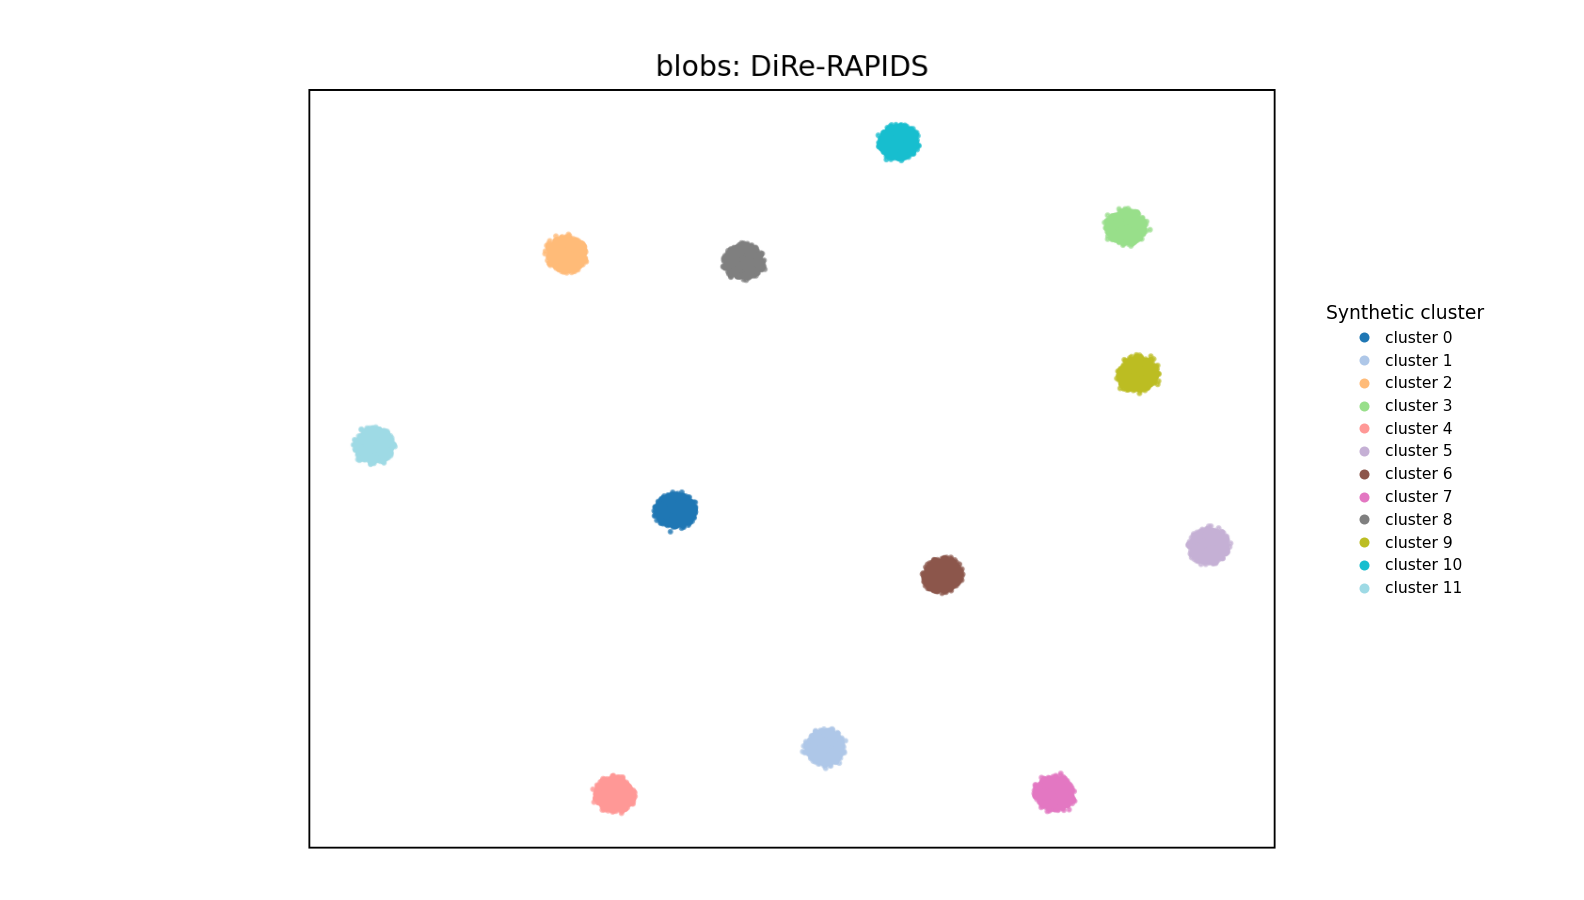
\includegraphics[width=\textwidth]{pics/embeddings/blobs-dire-rapids.png}
        \caption{DiRe--RAPIDS}
        \label{fig:blobs-dire-rapids}
    \end{subfigure}
    \hfill
    \begin{subfigure}[b]{0.45\textwidth}
        \centering
        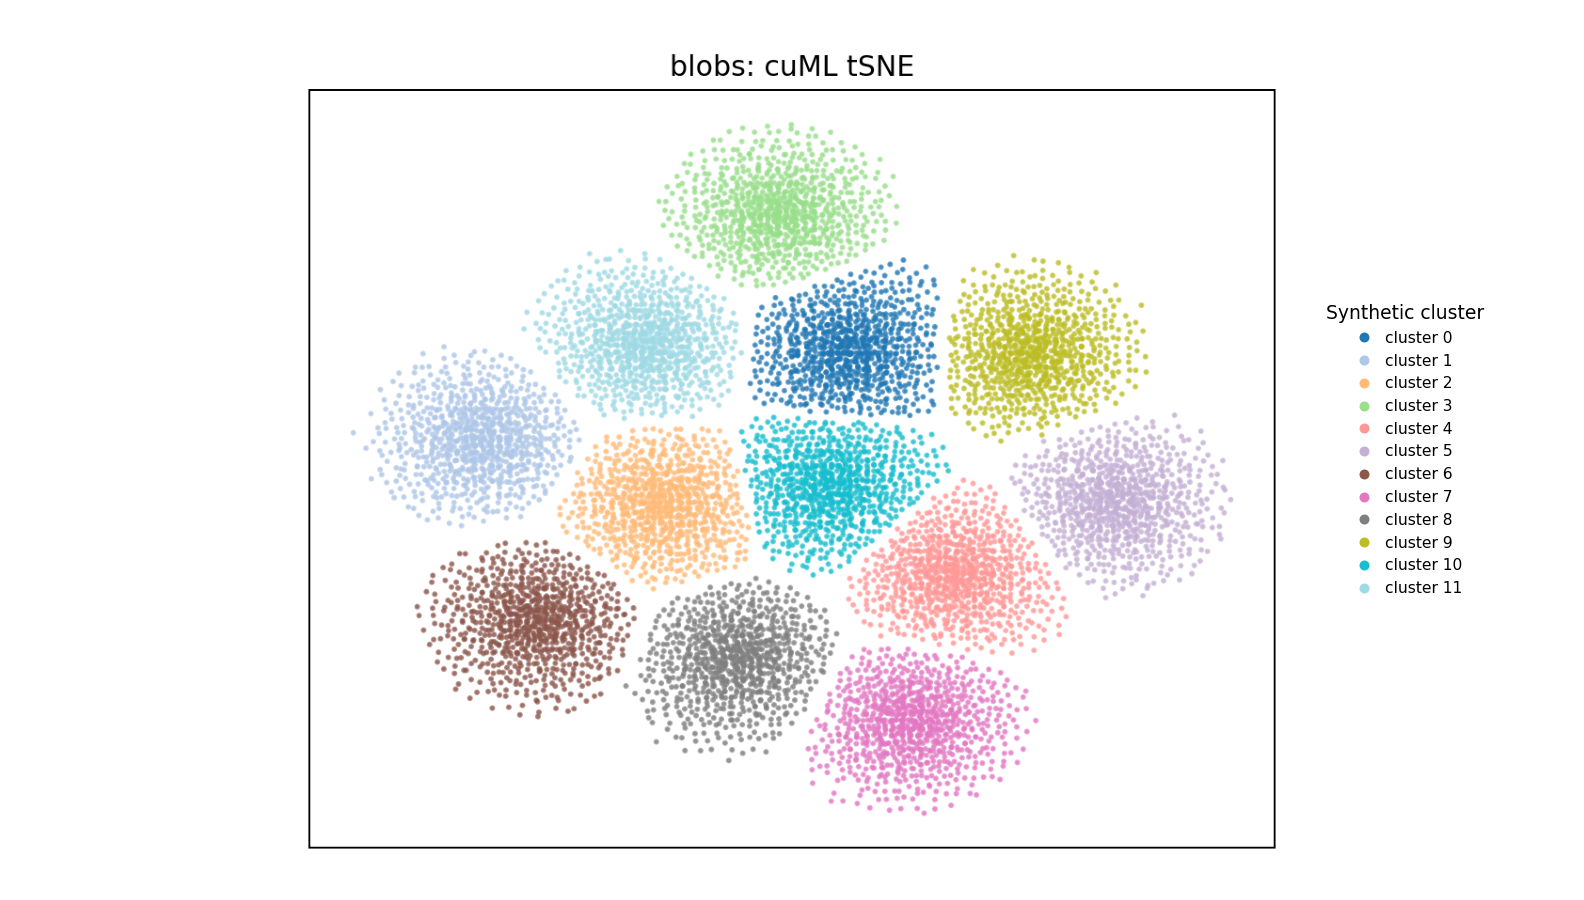
\includegraphics[width=\textwidth]{pics/embeddings/blobs-tsne.png}
        \caption{cuML tSNE}
        \label{fig:blobs-tsne}
    \end{subfigure}
    \vspace{1em}
    \begin{subfigure}[b]{0.45\textwidth}
        \centering
        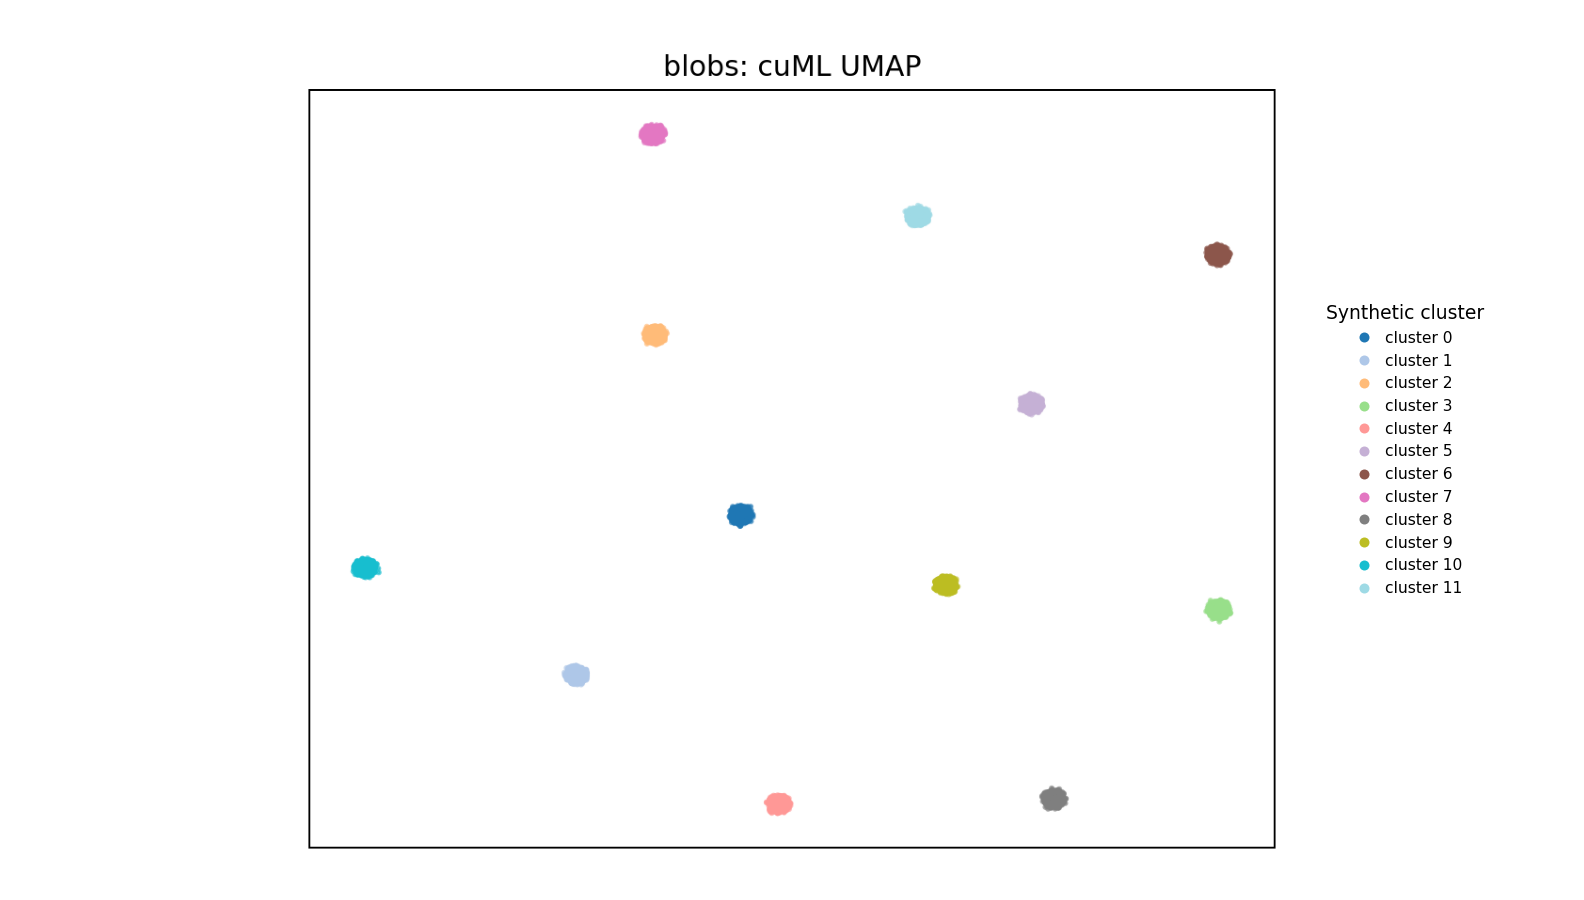
\includegraphics[width=\textwidth]{pics/embeddings/blobs-cuml-umap.png}
        \caption{cuML UMAP}
        \label{fig:blobs-cuml-umap}
    \end{subfigure}
    \hfill
    \begin{subfigure}[b]{0.45\textwidth}
        \centering
        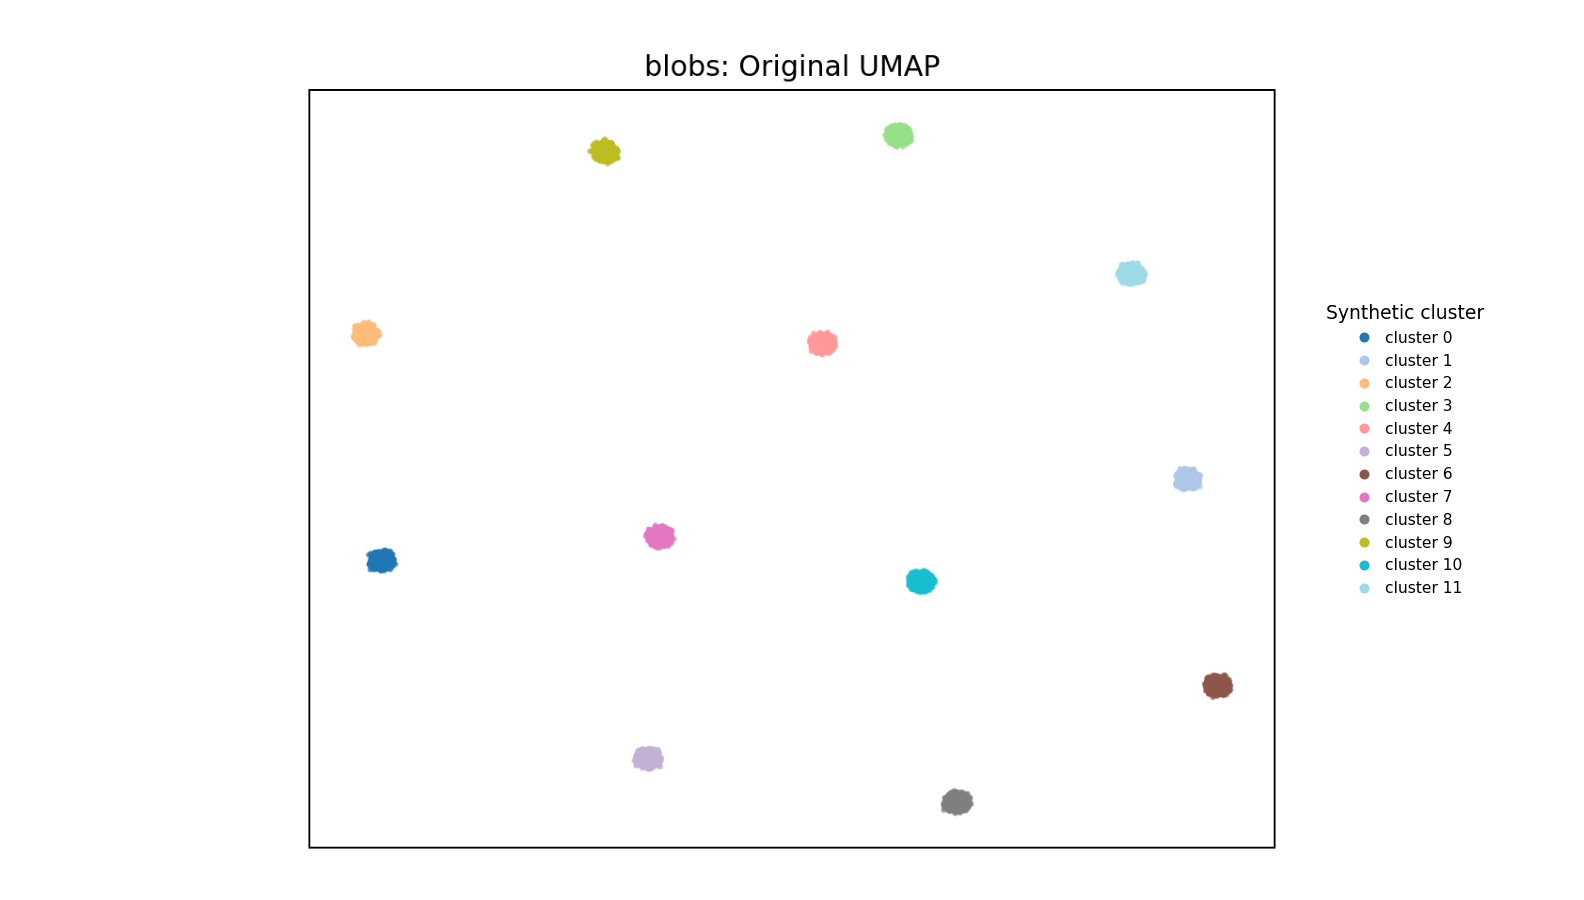
\includegraphics[width=\textwidth]{pics/embeddings/blobs-umap.png}
        \caption{Original UMAP}
        \label{fig:blobs-umap}
    \end{subfigure}
    \caption{"Blobs" dataset embeddings}
    \label{fig:blobs}
\end{figure}


\subsection{Dataset: MNIST Digits}

MNIST Digits provides a labeled image benchmark with well known class structure. This benchmark compares whether the methods preserve digit classes, transitions between visually similar digits, and the persistent homology summaries of the high--dimensional data.

The key metrics are given in Appendix~\ref{appendix:mnist}. In this dataset, visual cluster separation, classifier context, and persistence distances need not induce the same ranking, so these criteria are reported separately.

Even when all methods reasonably preserve labeled context, the SVM and kNN context scores can distinguish linear separability from local class consistency.

\begin{figure}[h]
    \centering
    \begin{subfigure}[b]{0.45\textwidth}
        \centering
        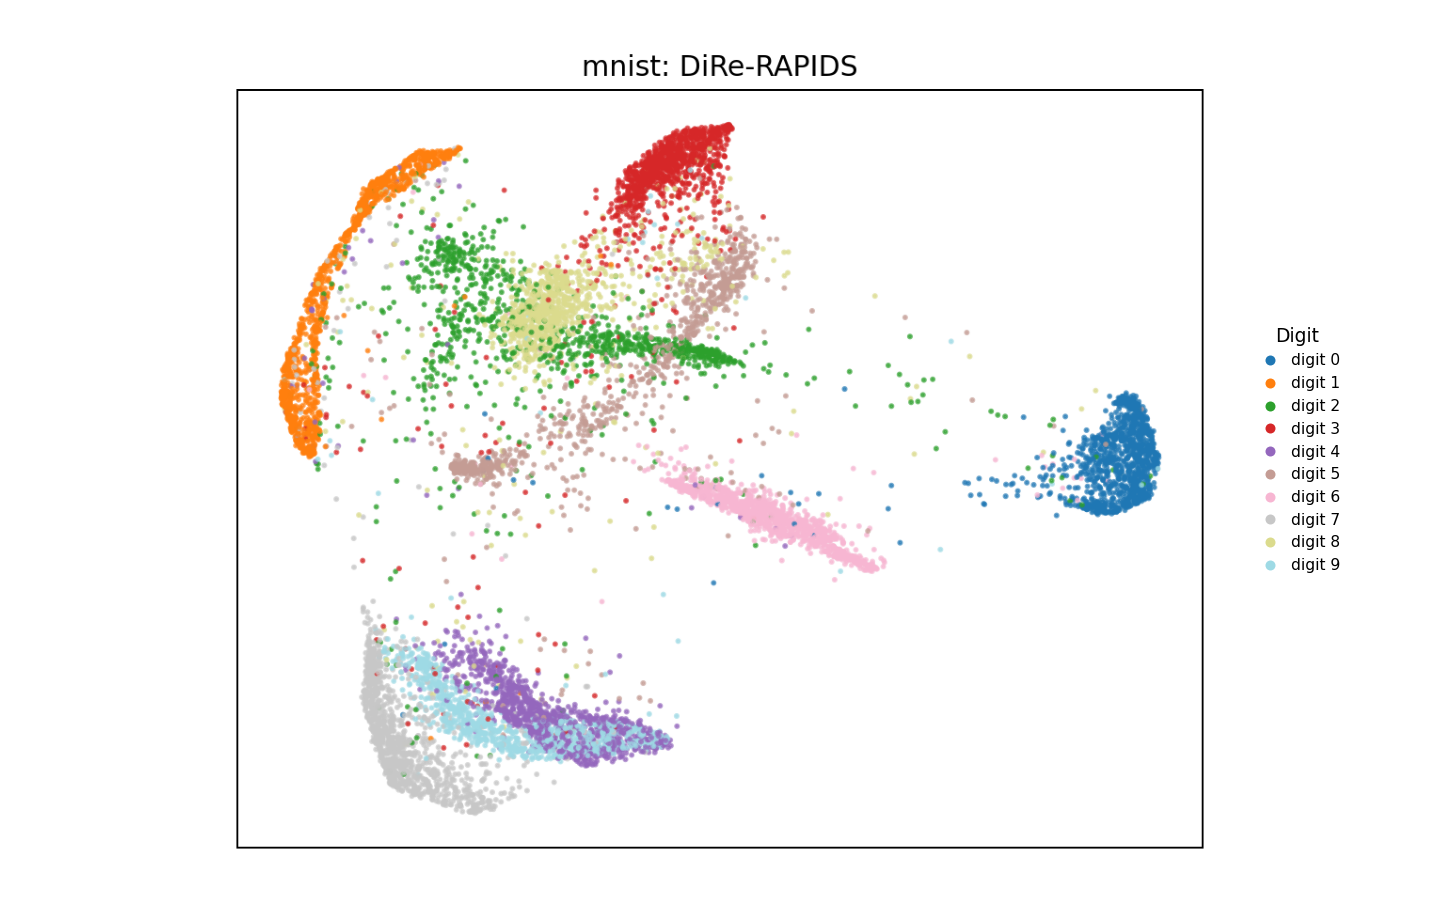
\includegraphics[width=\textwidth]{pics/embeddings/mnist-dire-rapids.png}
        \caption{DiRe--RAPIDS}
        \label{fig:mnist-dire-rapids}
    \end{subfigure}
    \hfill
    \begin{subfigure}[b]{0.45\textwidth}
        \centering
        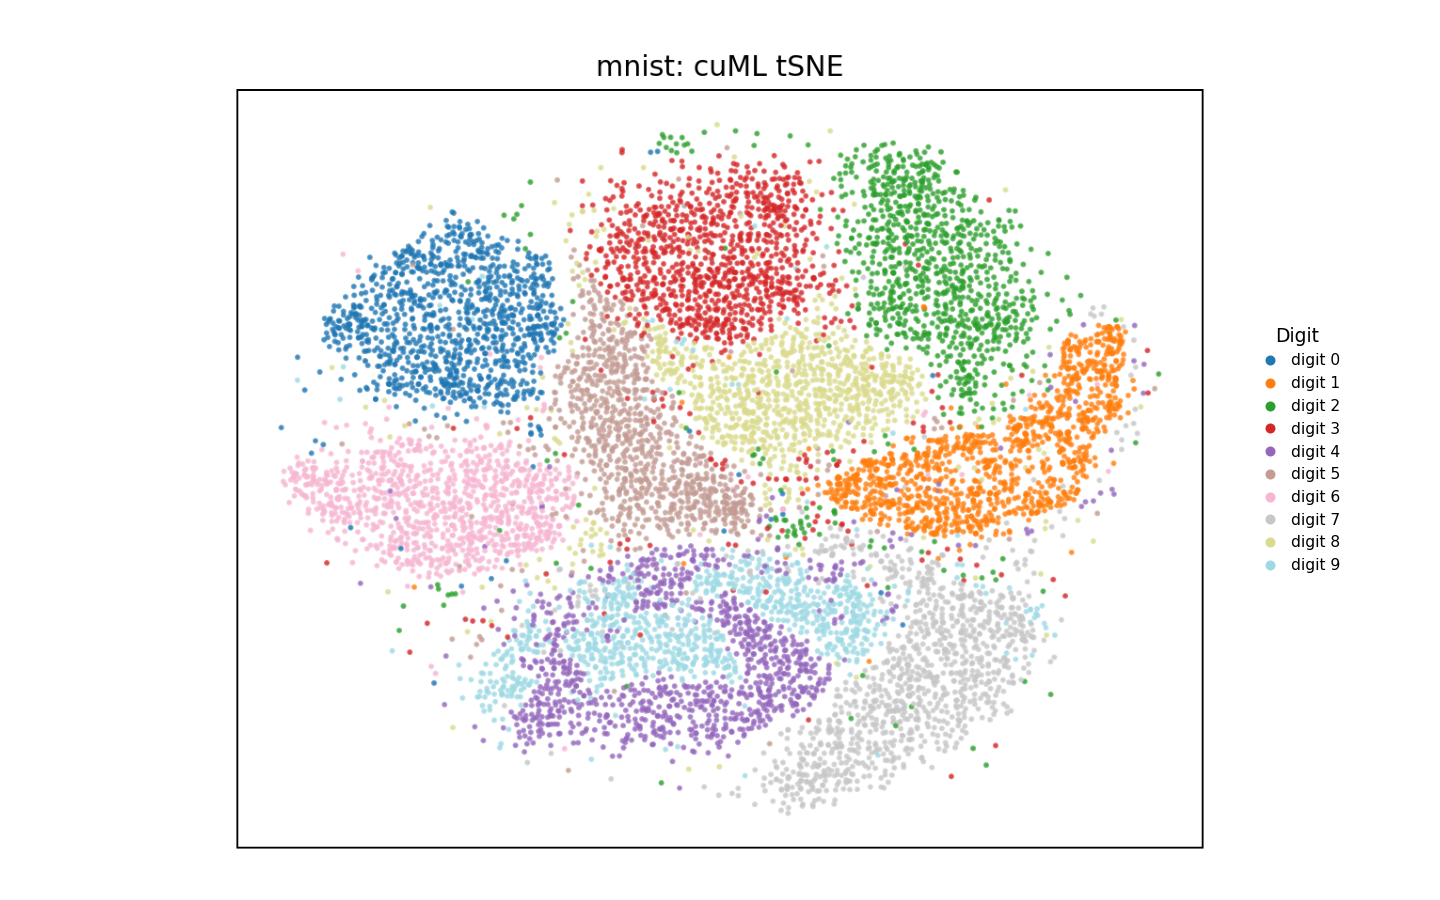
\includegraphics[width=\textwidth]{pics/embeddings/mnist-tsne.png}
        \caption{cuML tSNE}
        \label{fig:mnist-tsne}
    \end{subfigure}
    \vspace{1em}
    \begin{subfigure}[b]{0.45\textwidth}
        \centering
        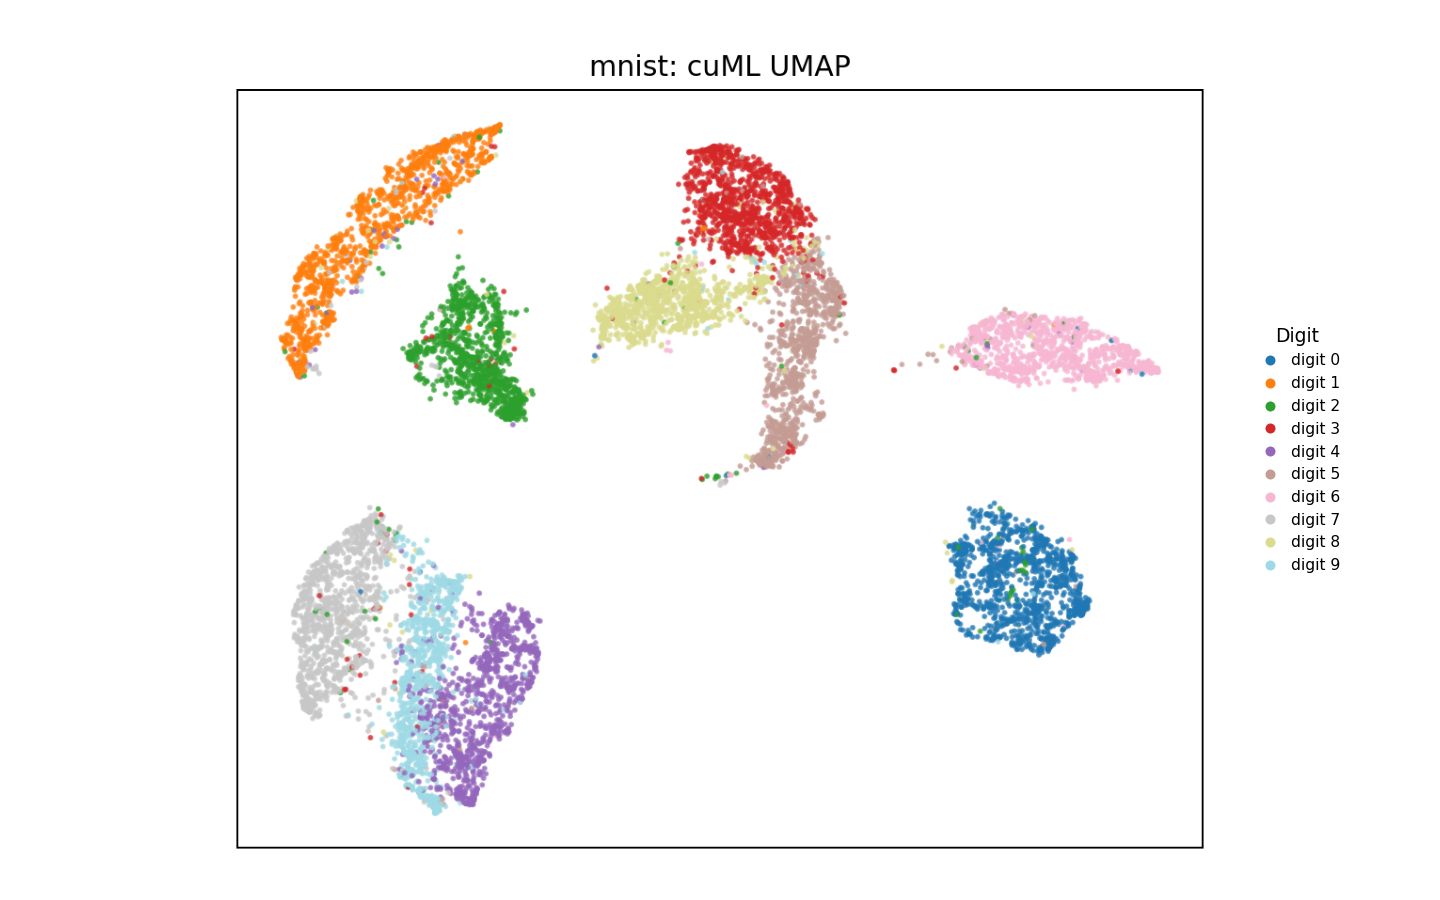
\includegraphics[width=\textwidth]{pics/embeddings/mnist-cuml-umap.png}
        \caption{cuML UMAP}
        \label{fig:mnist-cuml-umap}
    \end{subfigure}
    \hfill
    \begin{subfigure}[b]{0.45\textwidth}
        \centering
        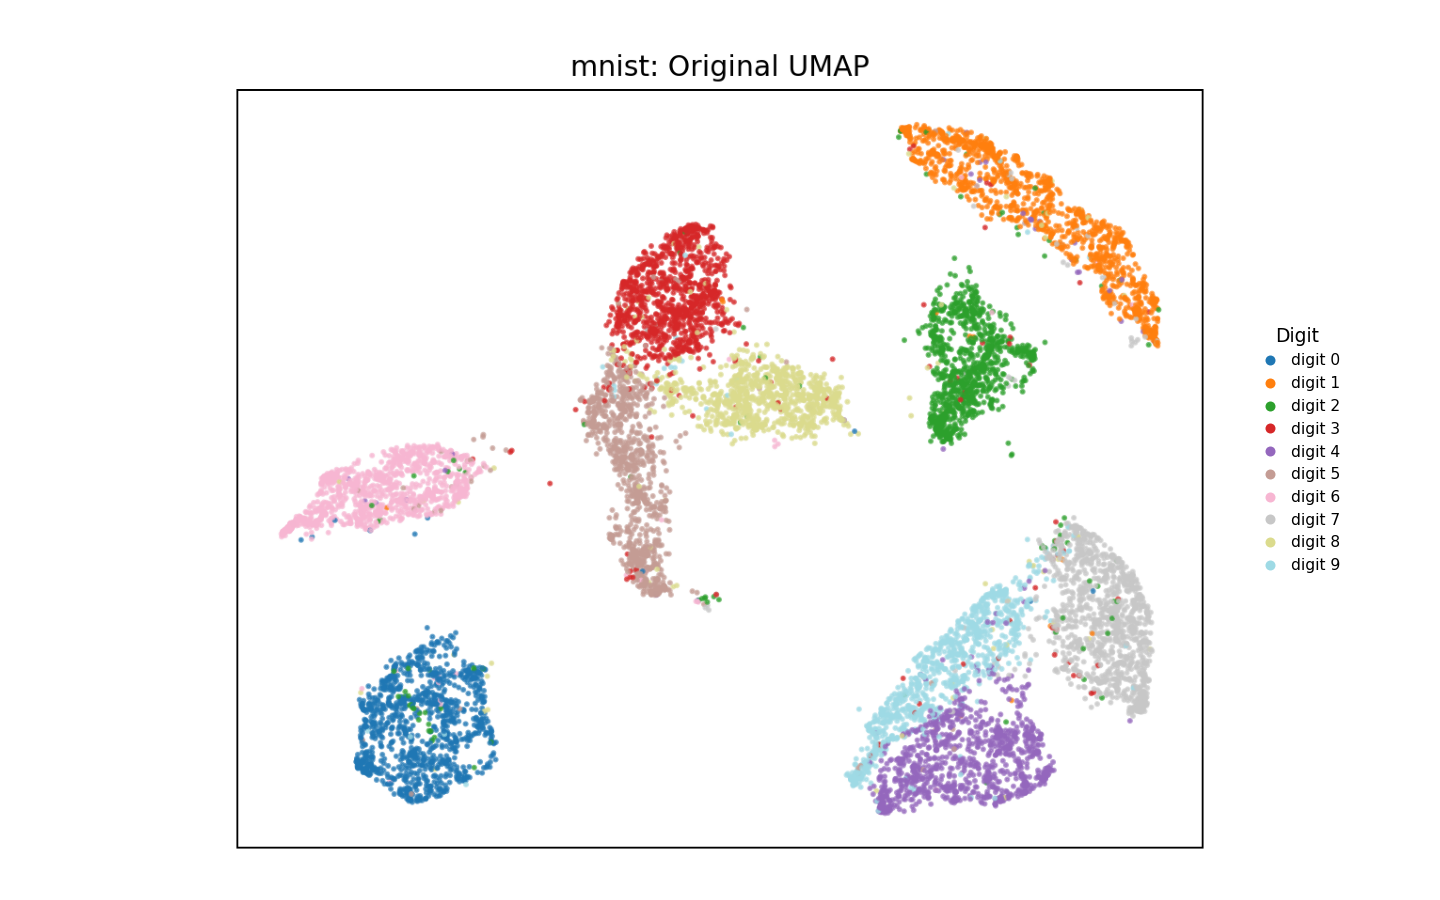
\includegraphics[width=\textwidth]{pics/embeddings/mnist-umap.png}
        \caption{Original UMAP}
        \label{fig:mnist-umap}
    \end{subfigure}
    \caption{"MNIST Digits" dataset embeddings}
    \label{fig:mnist}
\end{figure} 

\subsection{Dataset: Disk Uniform}

Here we embed a 2D disk with points uniformly distributed in it. Since the input already has a simple low--dimensional geometry, this benchmark tests whether a method unnecessarily distorts connectedness, density, or boundary shape.

A similar family of tests can be run on a sphere and an ellipsoid in 3D with uniformly distributed points. See the DiRe--RAPIDS repository for additional datasets \cite{dire-rapids}.

The metrics are given in Appendix~\ref{appendix:disk}. We treat persistence metrics and local distortion metrics as complementary: a method may preserve nearest neighbors while changing the global shape of this simple input.

\begin{figure}[ht]
    \centering
    \begin{subfigure}[b]{0.45\textwidth}
        \centering
        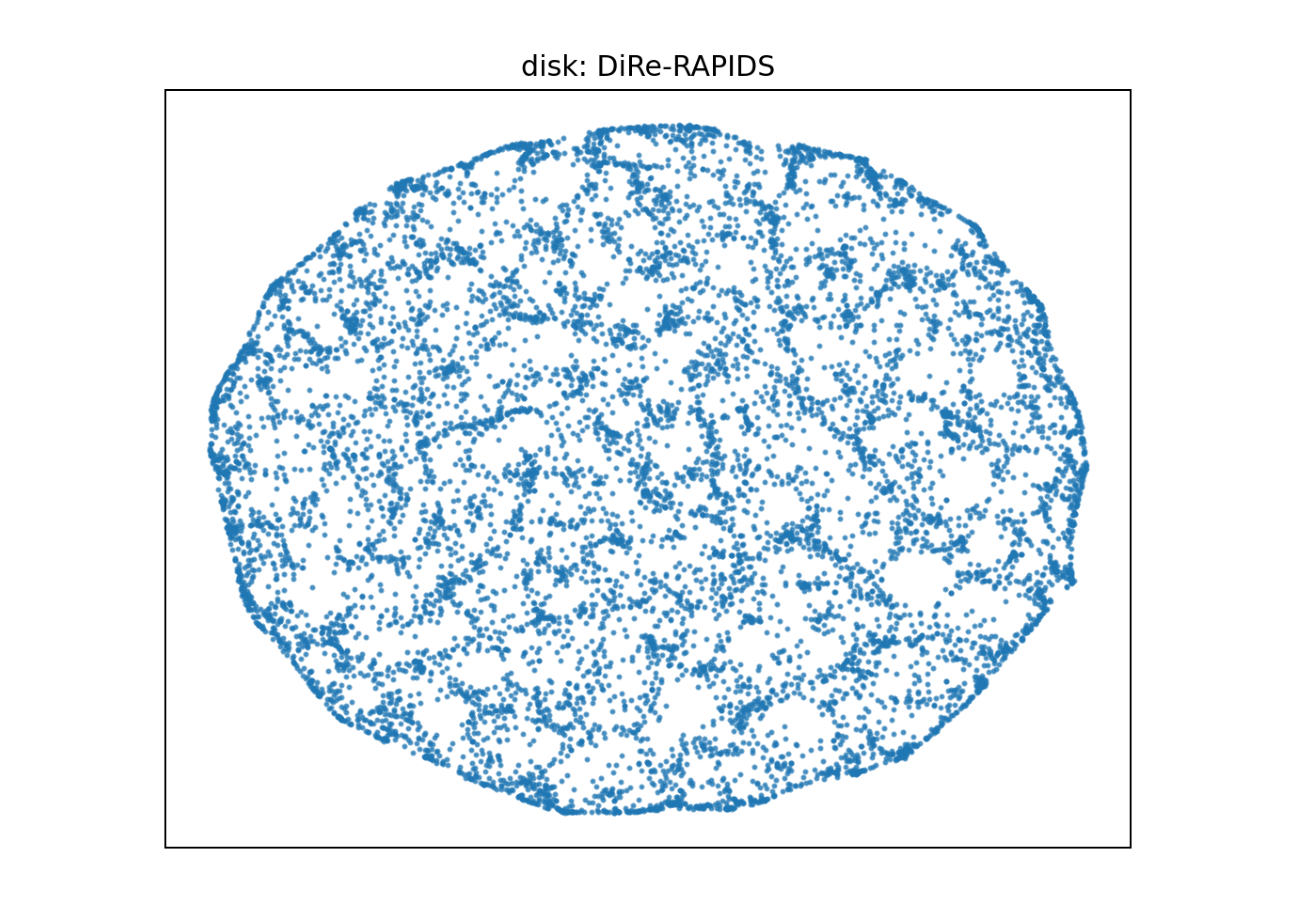
\includegraphics[width=\textwidth]{pics/embeddings/disk-dire-rapids.png}
        \caption{DiRe--RAPIDS}
        \label{fig:disk-dire-rapids}
    \end{subfigure}
    \hfill
    \begin{subfigure}[b]{0.45\textwidth}
        \centering
        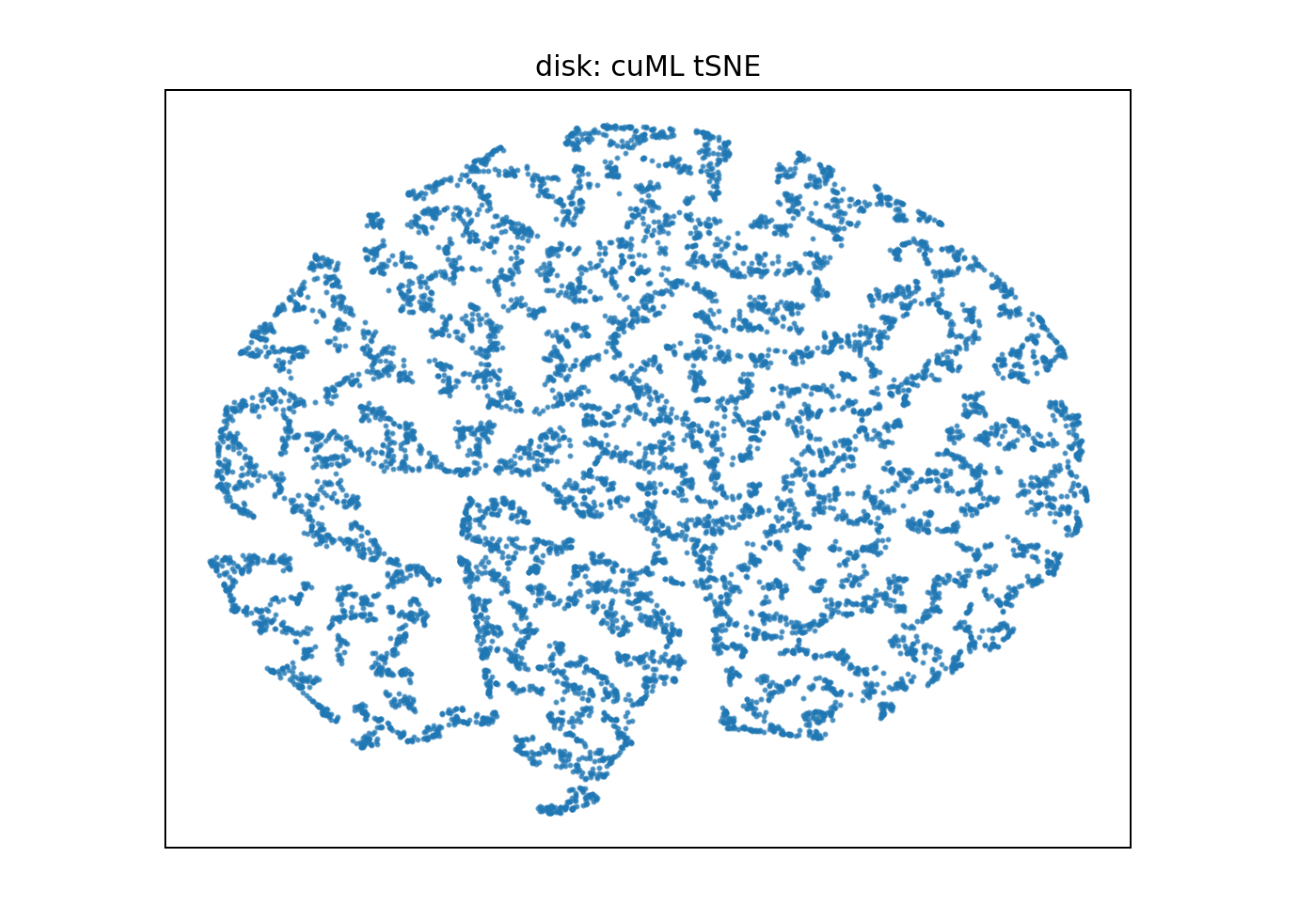
\includegraphics[width=\textwidth]{pics/embeddings/disk-tsne.png}
        \caption{cuML tSNE}
        \label{fig:disk-tsne}
    \end{subfigure}
    \vspace{1em}
    \begin{subfigure}[b]{0.45\textwidth}
        \centering
        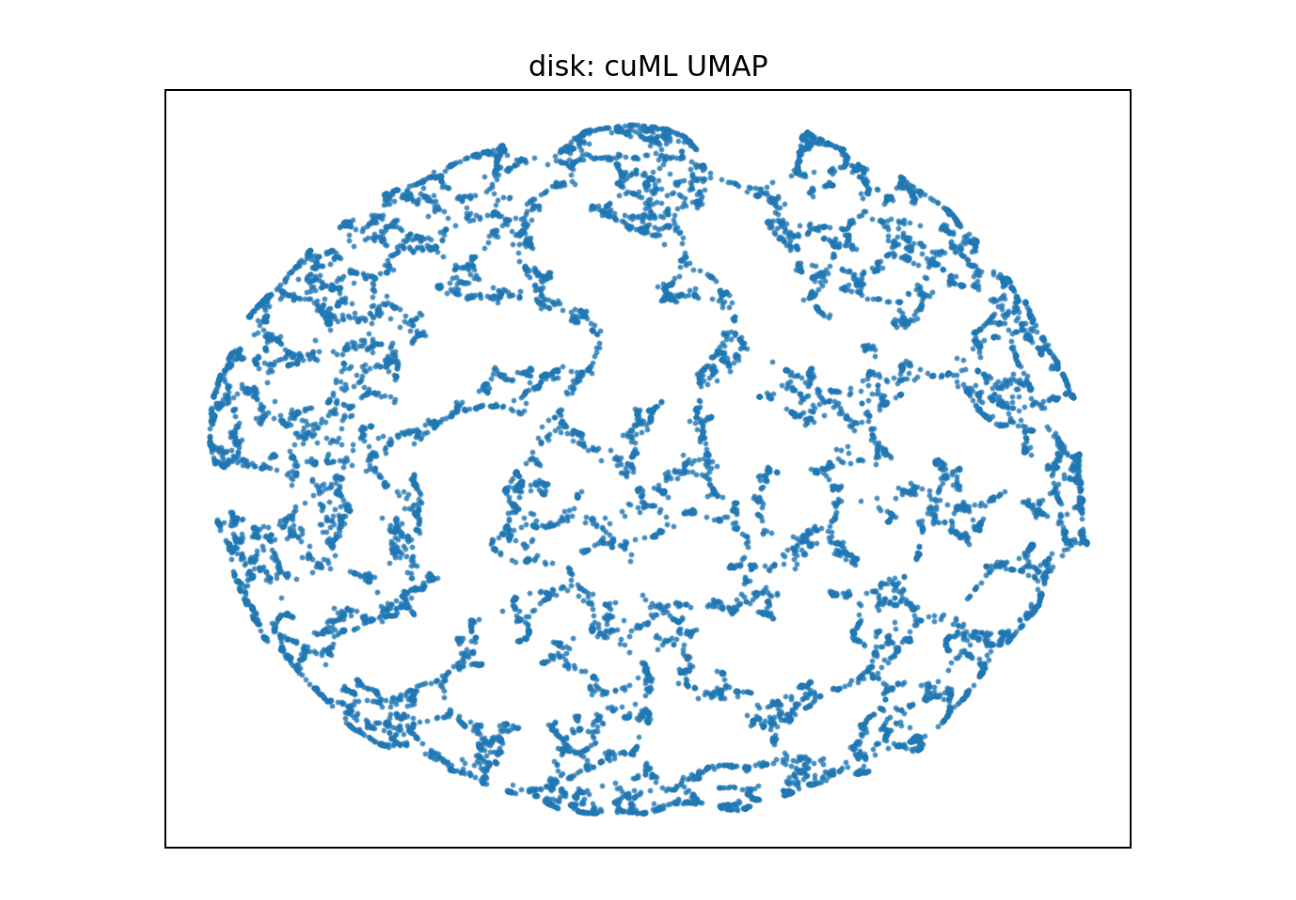
\includegraphics[width=\textwidth]{pics/embeddings/disk-cuml-umap.png}
        \caption{cuML UMAP}
        \label{fig:disk-cuml-umap}
    \end{subfigure}
    \hfill
    \begin{subfigure}[b]{0.45\textwidth}
        \centering
        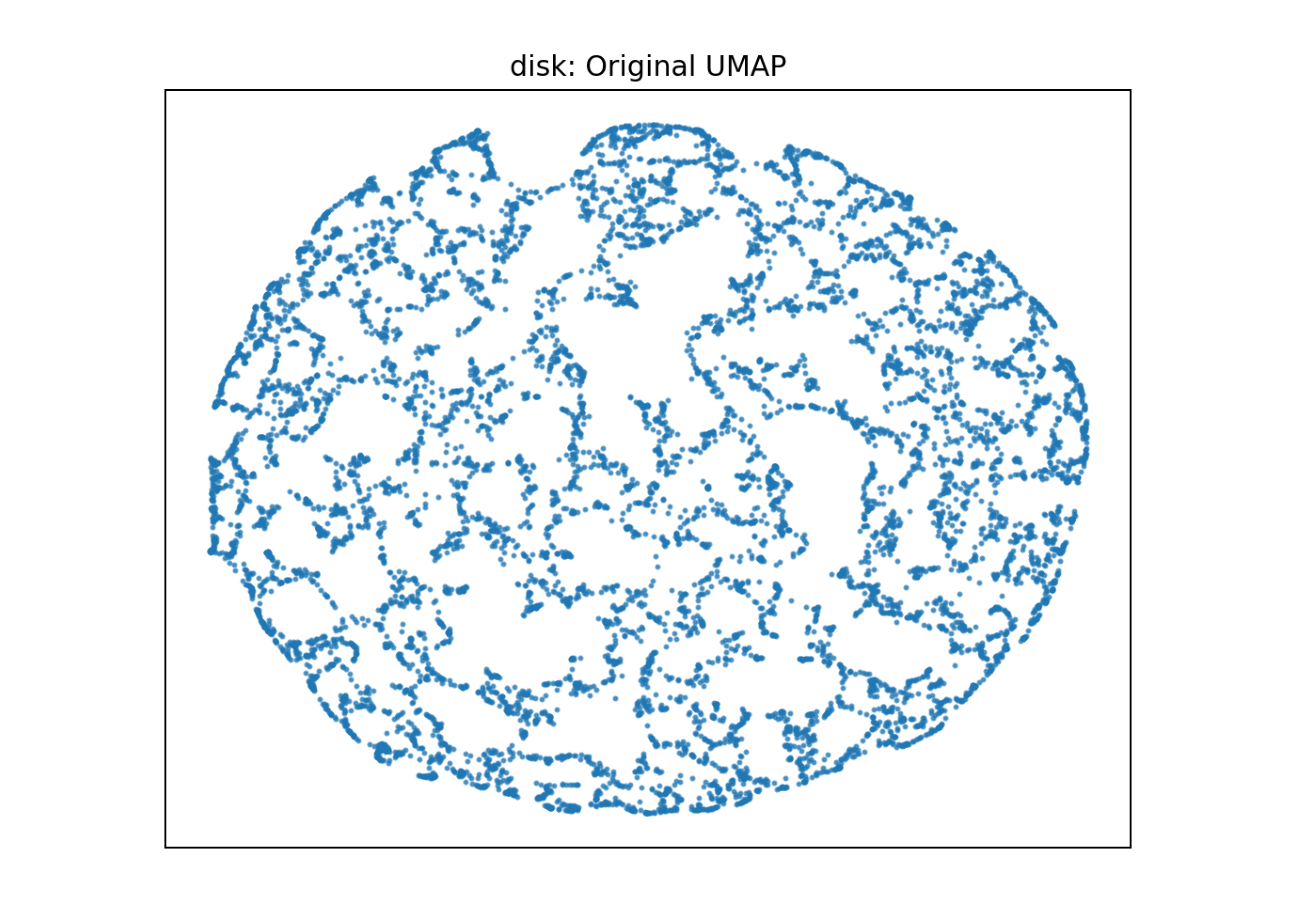
\includegraphics[width=\textwidth]{pics/embeddings/disk-umap.png}
        \caption{Original UMAP}
        \label{fig:disk-umap}
    \end{subfigure}
    \caption{"Disk Uniform" dataset embeddings}
    \label{fig:disk}
\end{figure}

\subsection{Dataset: Half-moons}

The half--moons dataset tests whether a method preserves the non--linear relation between two labeled components. Since the input classes are not linearly separable, a two--dimensional embedding that makes them linearly separable may improve a downstream classifier while changing the original context. The context preservation score is reported in Appendix~\ref{appendix:moons}.

\begin{figure}[ht]
    \centering
    \begin{subfigure}[b]{0.45\textwidth}
        \centering
        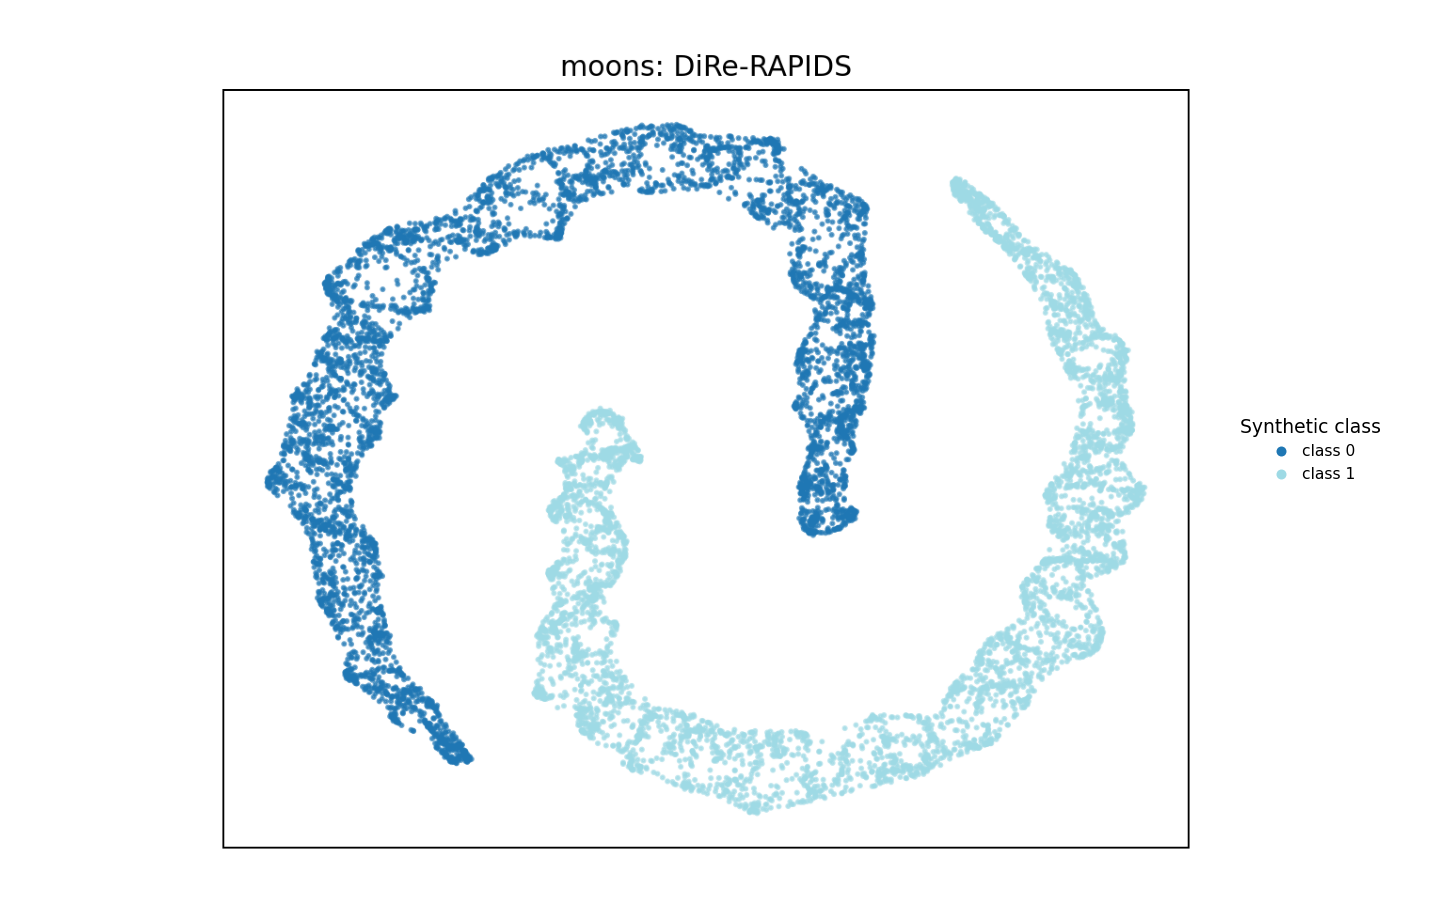
\includegraphics[width=\textwidth]{pics/embeddings/moons-dire-rapids.png}
        \caption{DiRe--RAPIDS}
        \label{fig:moons-dire-rapids}
    \end{subfigure}
    \hfill
    \begin{subfigure}[b]{0.45\textwidth}
        \centering
        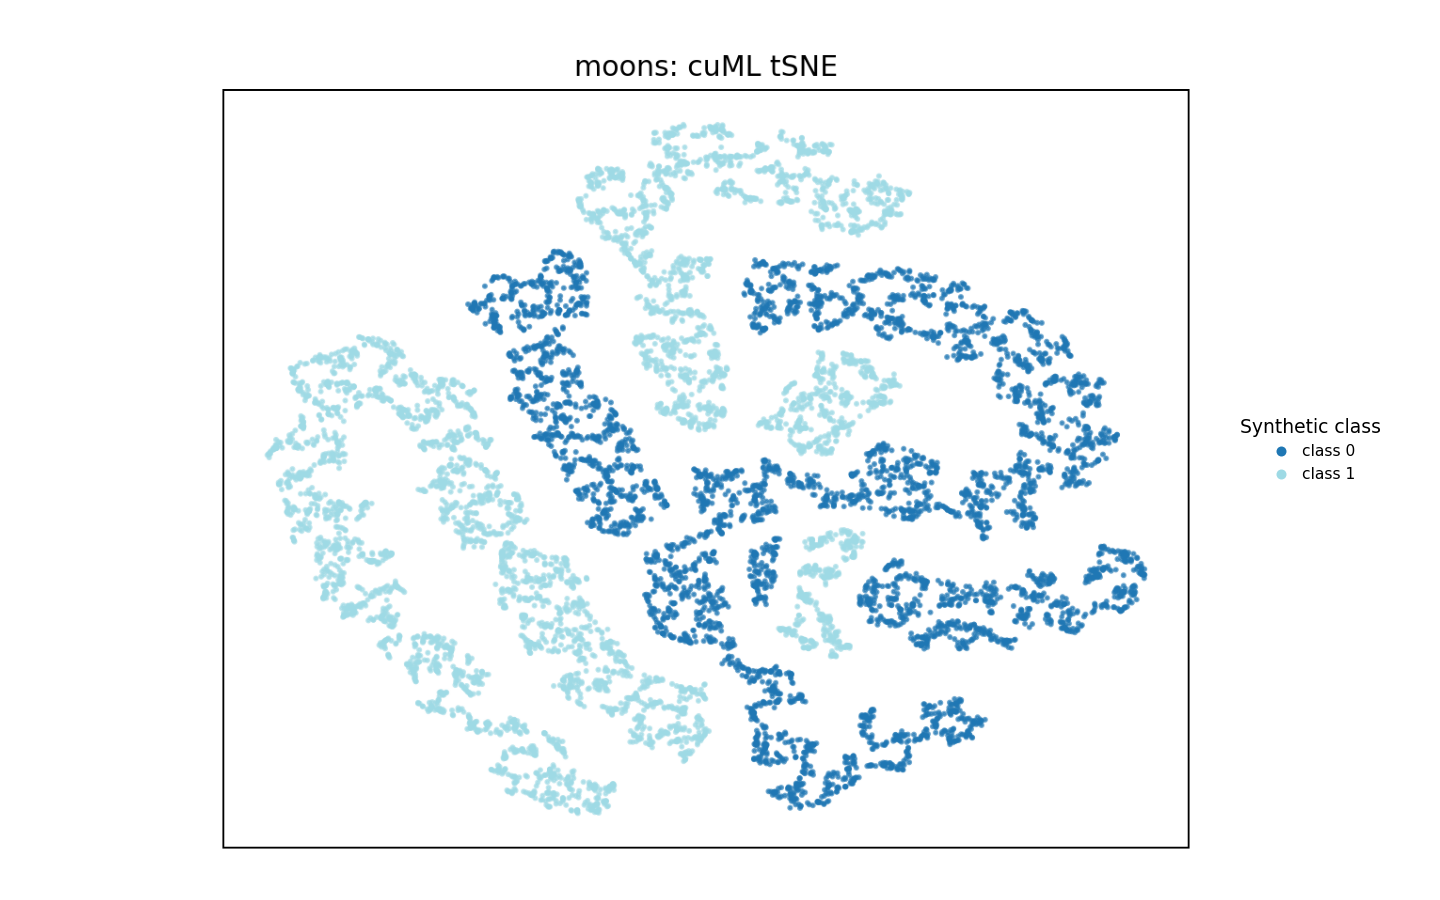
\includegraphics[width=\textwidth]{pics/embeddings/moons-tsne.png}
        \caption{cuML tSNE}
        \label{fig:moons-tsne}
    \end{subfigure}
    \vspace{1em}
    \begin{subfigure}[b]{0.45\textwidth}
        \centering
        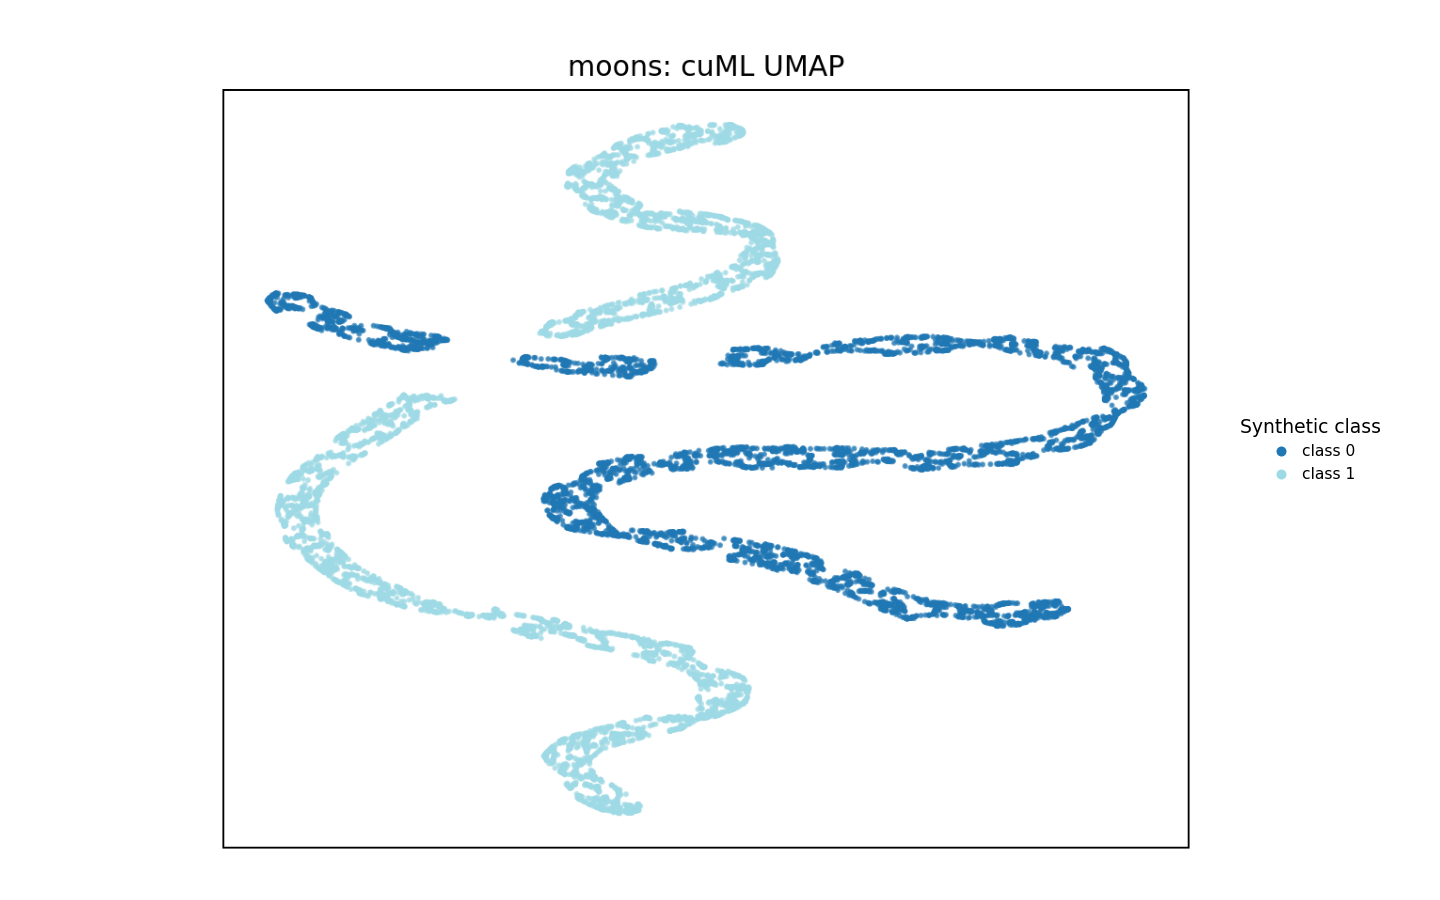
\includegraphics[width=\textwidth]{pics/embeddings/moons-cuml-umap.png}
        \caption{cuML UMAP}
        \label{fig:moons-cuml-umap}
    \end{subfigure}
    \hfill
    \begin{subfigure}[b]{0.45\textwidth}
        \centering
        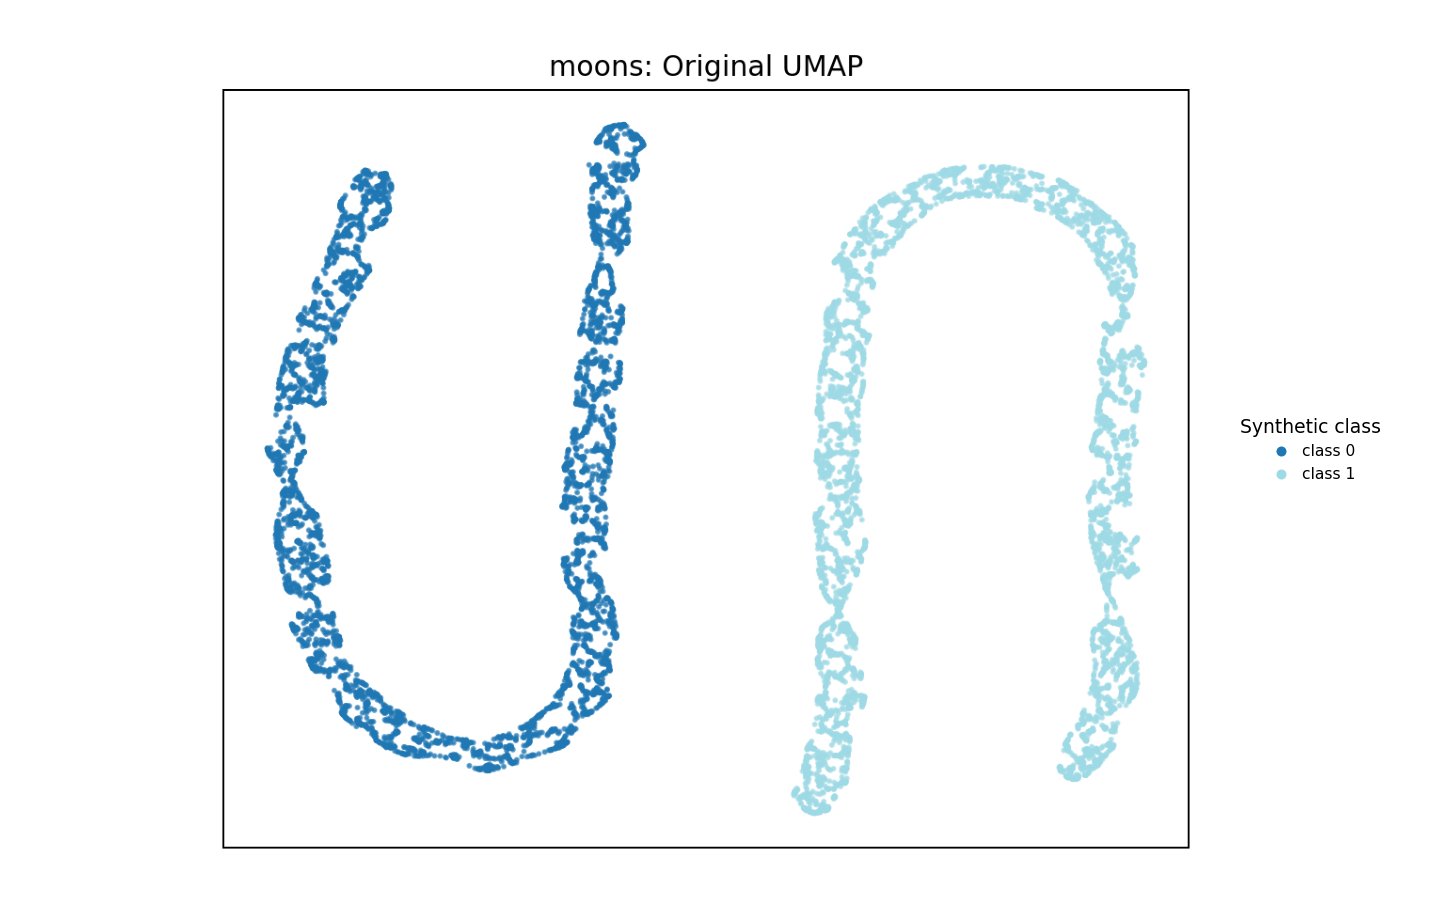
\includegraphics[width=\textwidth]{pics/embeddings/moons-umap.png}
        \caption{Original UMAP}
        \label{fig:moons-umap}
    \end{subfigure}
    \caption{"Two Half--Moons" dataset embeddings}
    \label{fig:moons}
\end{figure}

We compare the embeddings against both context metrics and persistence metrics, rather than relying on visual inspection alone.

\subsection{Dataset: Levine 13}

The Levine 13 CyTOF single--cell dataset serves as a biological benchmark in which preprocessing choices matter. In this benchmark, the expression channels are transformed with an inverse hyperbolic sine transform with cofactor 5; label and individual metadata columns are excluded from the feature matrix, and unassigned cells are removed.

\begin{figure}[ht]
    \centering
    \begin{subfigure}[b]{0.45\textwidth}
        \centering
        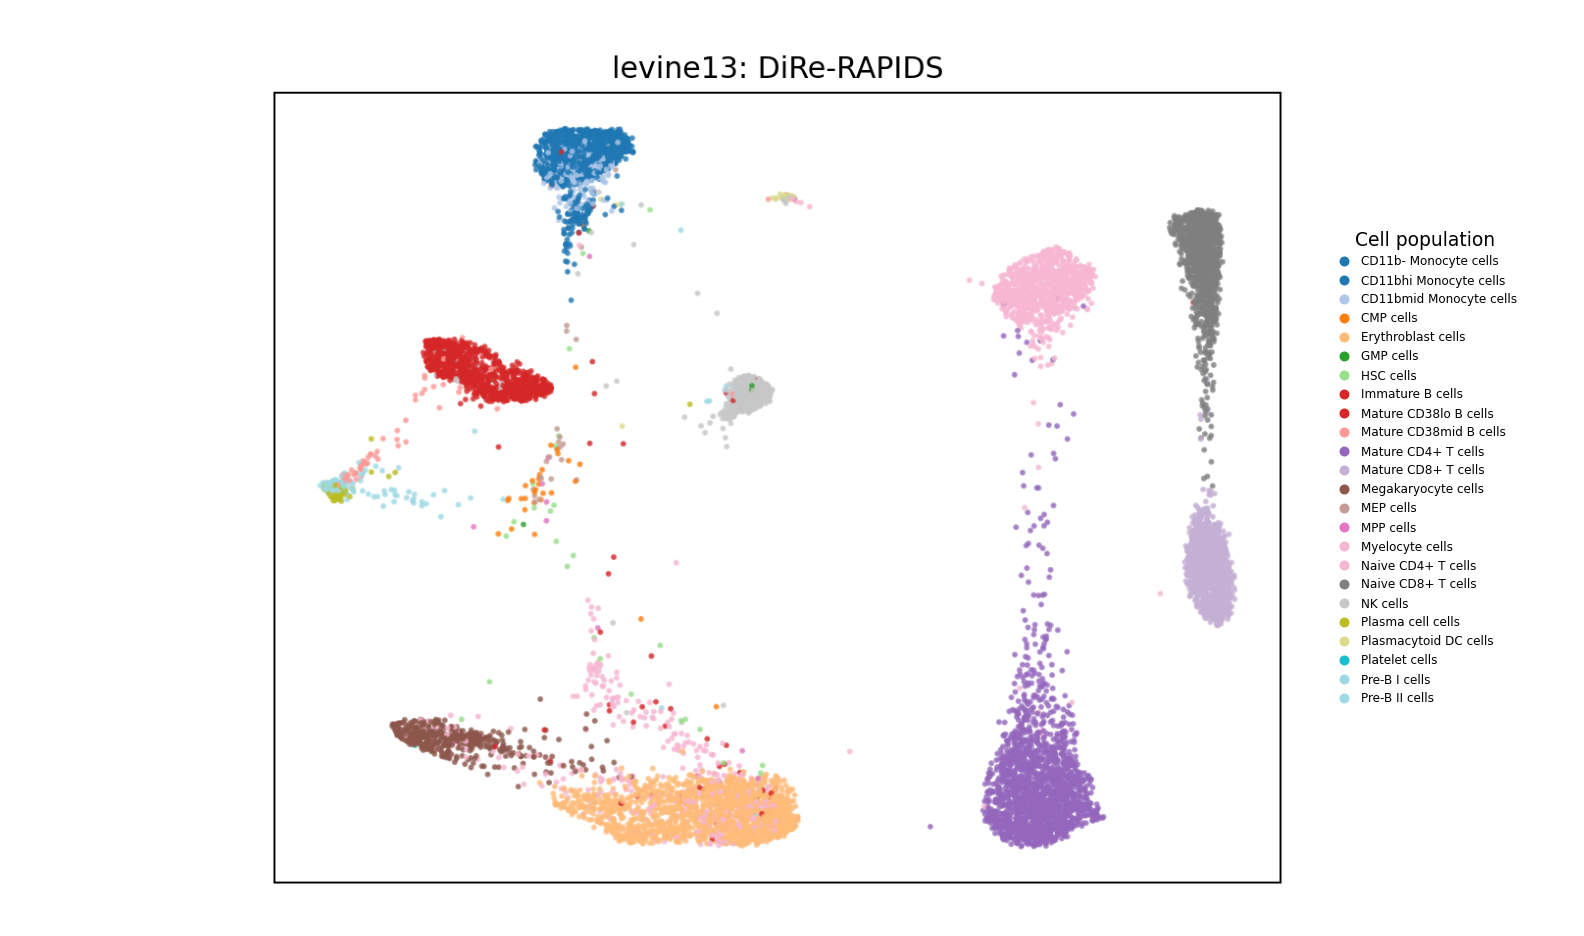
\includegraphics[width=\textwidth]{pics/embeddings/levine13-dire-rapids.png}
        \caption{DiRe--RAPIDS}
        \label{fig:lev13-dire-rapids}
    \end{subfigure}
    \hfill
    \begin{subfigure}[b]{0.45\textwidth}
        \centering
        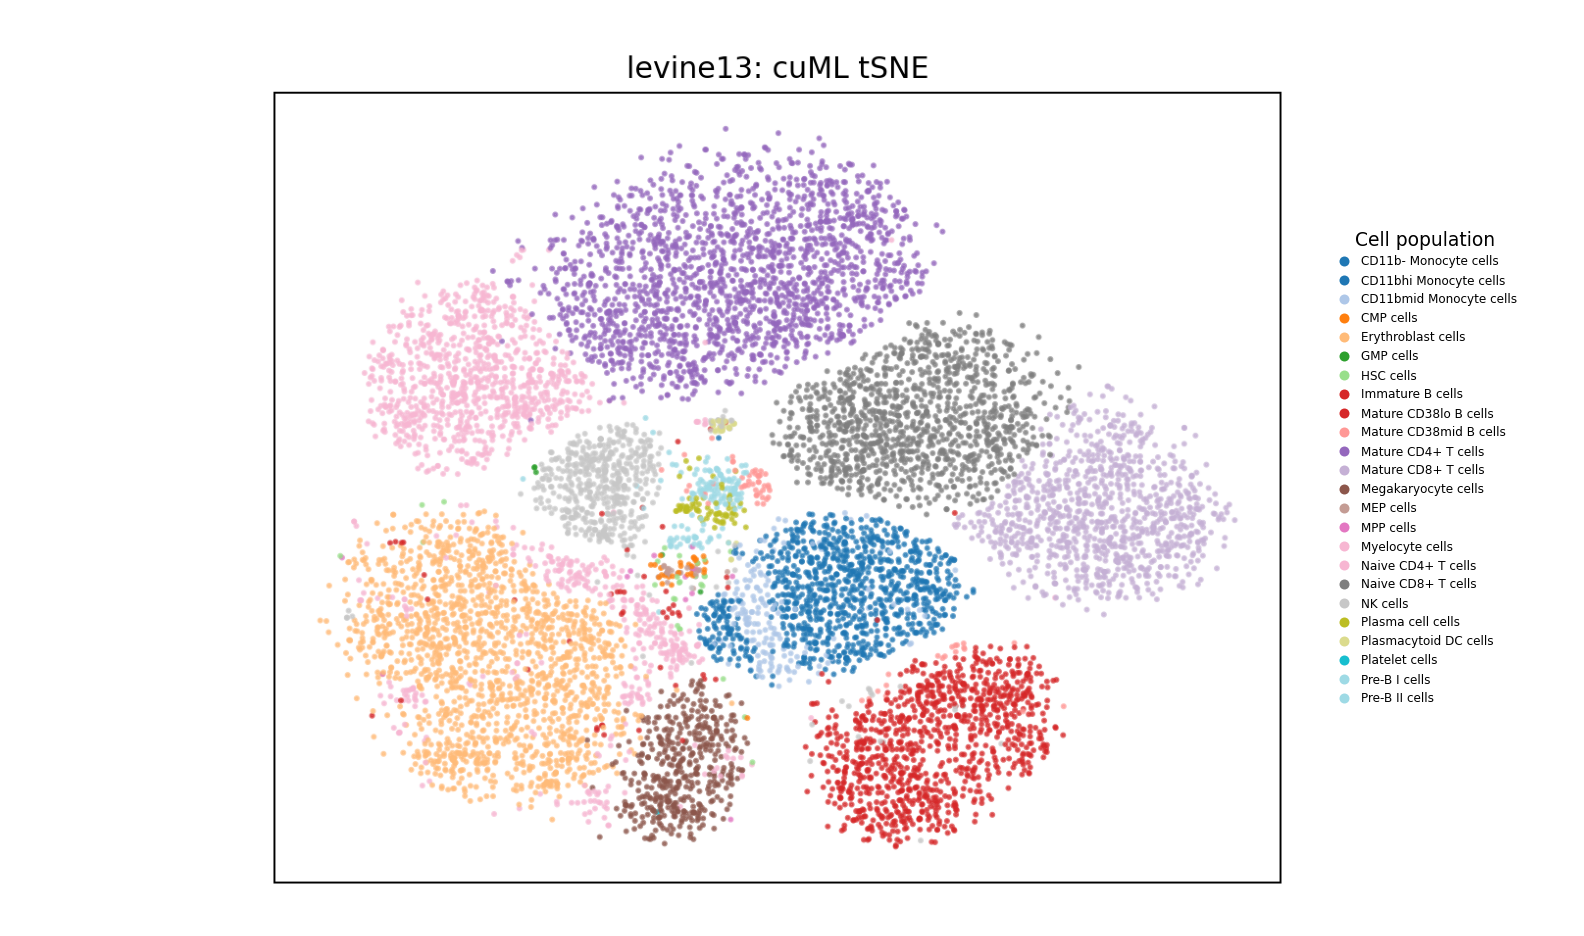
\includegraphics[width=\textwidth]{pics/embeddings/levine13-tsne.png}
        \caption{cuML tSNE}
        \label{fig:lev13-tsne}
    \end{subfigure}
    \vspace{1em}
    \begin{subfigure}[b]{0.45\textwidth}
        \centering
        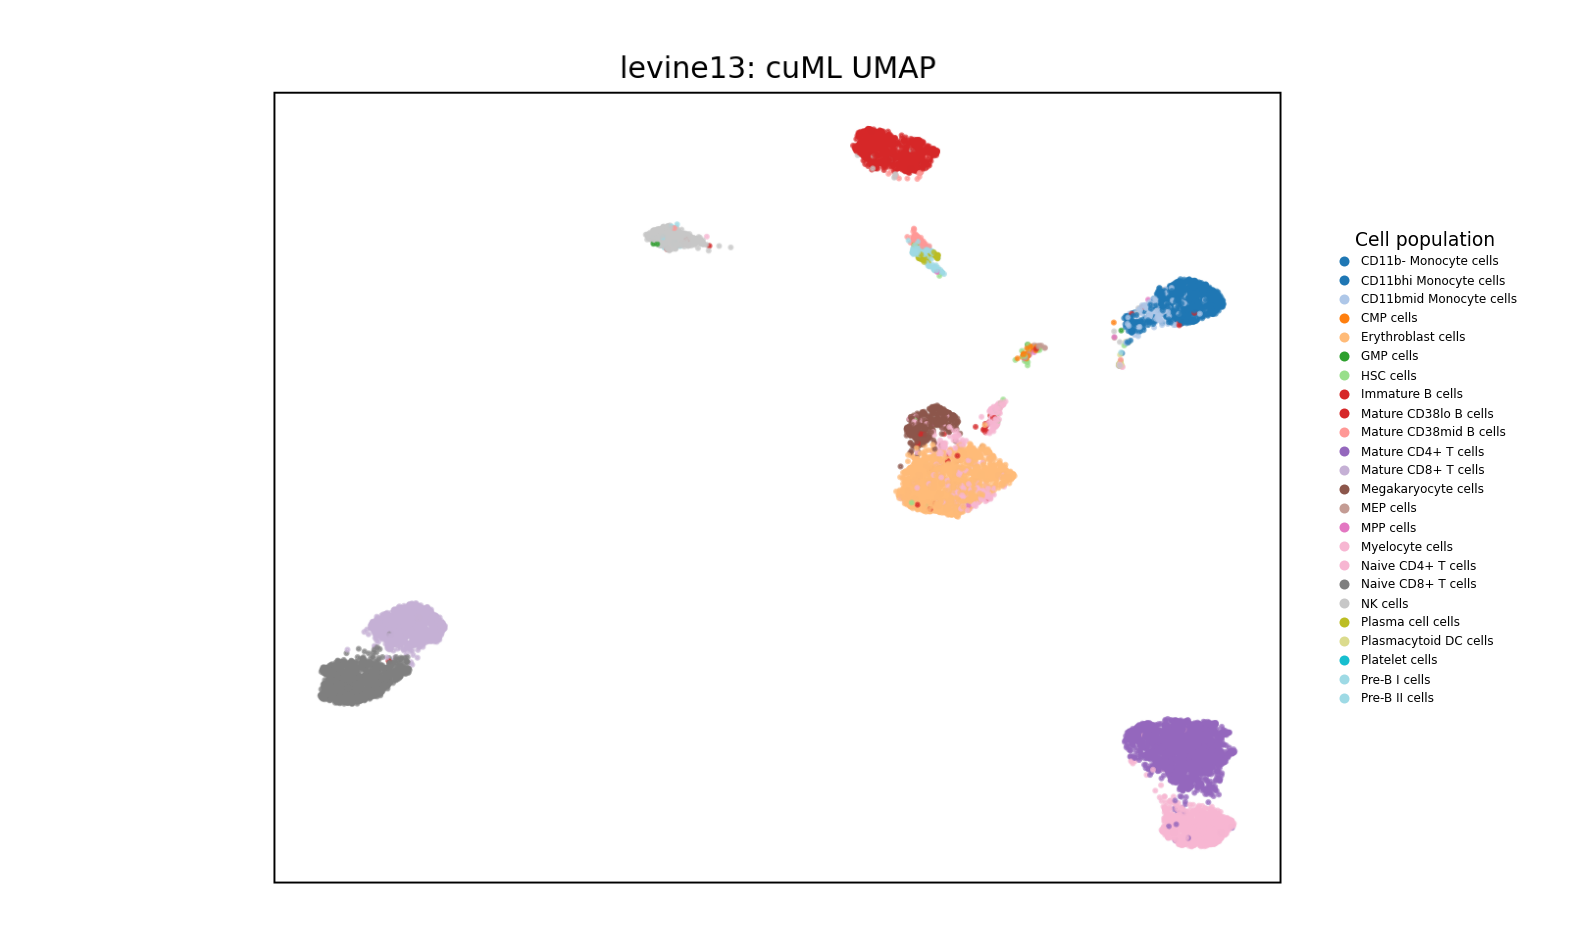
\includegraphics[width=\textwidth]{pics/embeddings/levine13-cuml-umap.png}
        \caption{cuML UMAP}
        \label{fig:lev13-cuml-umap}
    \end{subfigure}
    \hfill
    \begin{subfigure}[b]{0.45\textwidth}
        \centering
        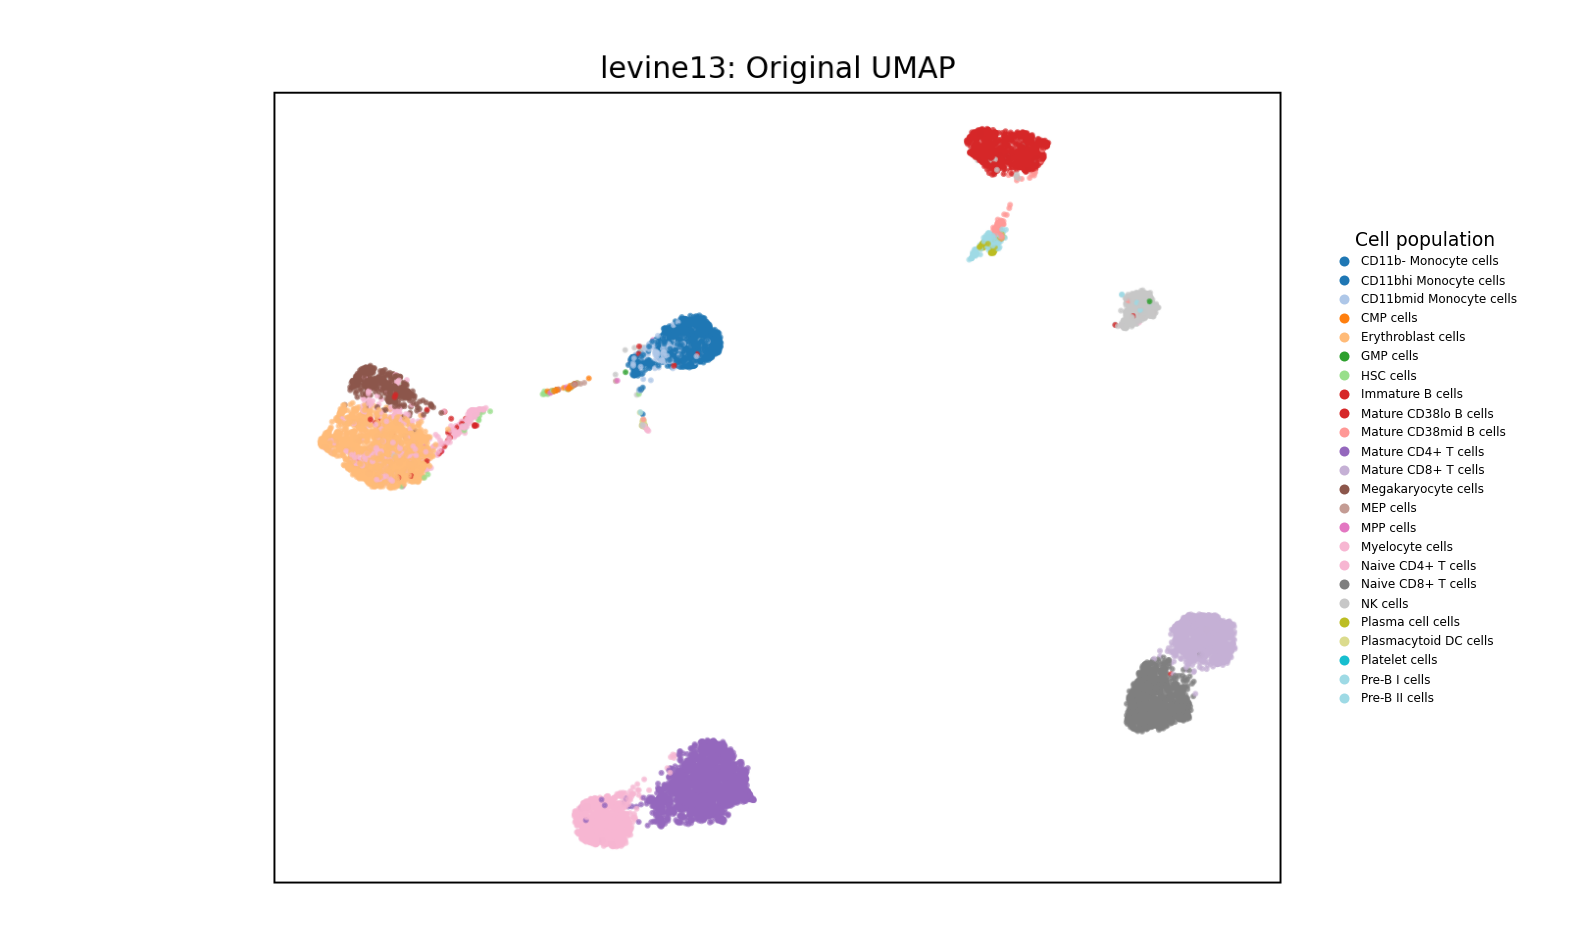
\includegraphics[width=\textwidth]{pics/embeddings/levine13-umap.png}
        \caption{Original UMAP}
        \label{fig:lev13-umap}
    \end{subfigure}
    \caption{"Levine 13" dataset embeddings}
    \label{fig:levine13}
\end{figure}

We report persistence and context metrics separately, since biological labels, local neighborhoods, and topological summaries need not agree perfectly.

More benchmarking information is available in Appendix~\ref{appendix:levine13}.

\subsection{Dataset: Levine 32}

The Levine 32 CyTOF dataset is handled with particular care because patient, batch, or other metadata columns can dominate an embedding if they are inadvertently included as numerical features. The same preprocessing protocol is used as for Levine 13: expression channels are arcsinh--transformed with cofactor 5, label and individual metadata columns are excluded from the feature matrix, and unassigned cells are removed.

\begin{figure}[ht]
    \centering
    \begin{subfigure}[b]{0.45\textwidth}
        \centering
        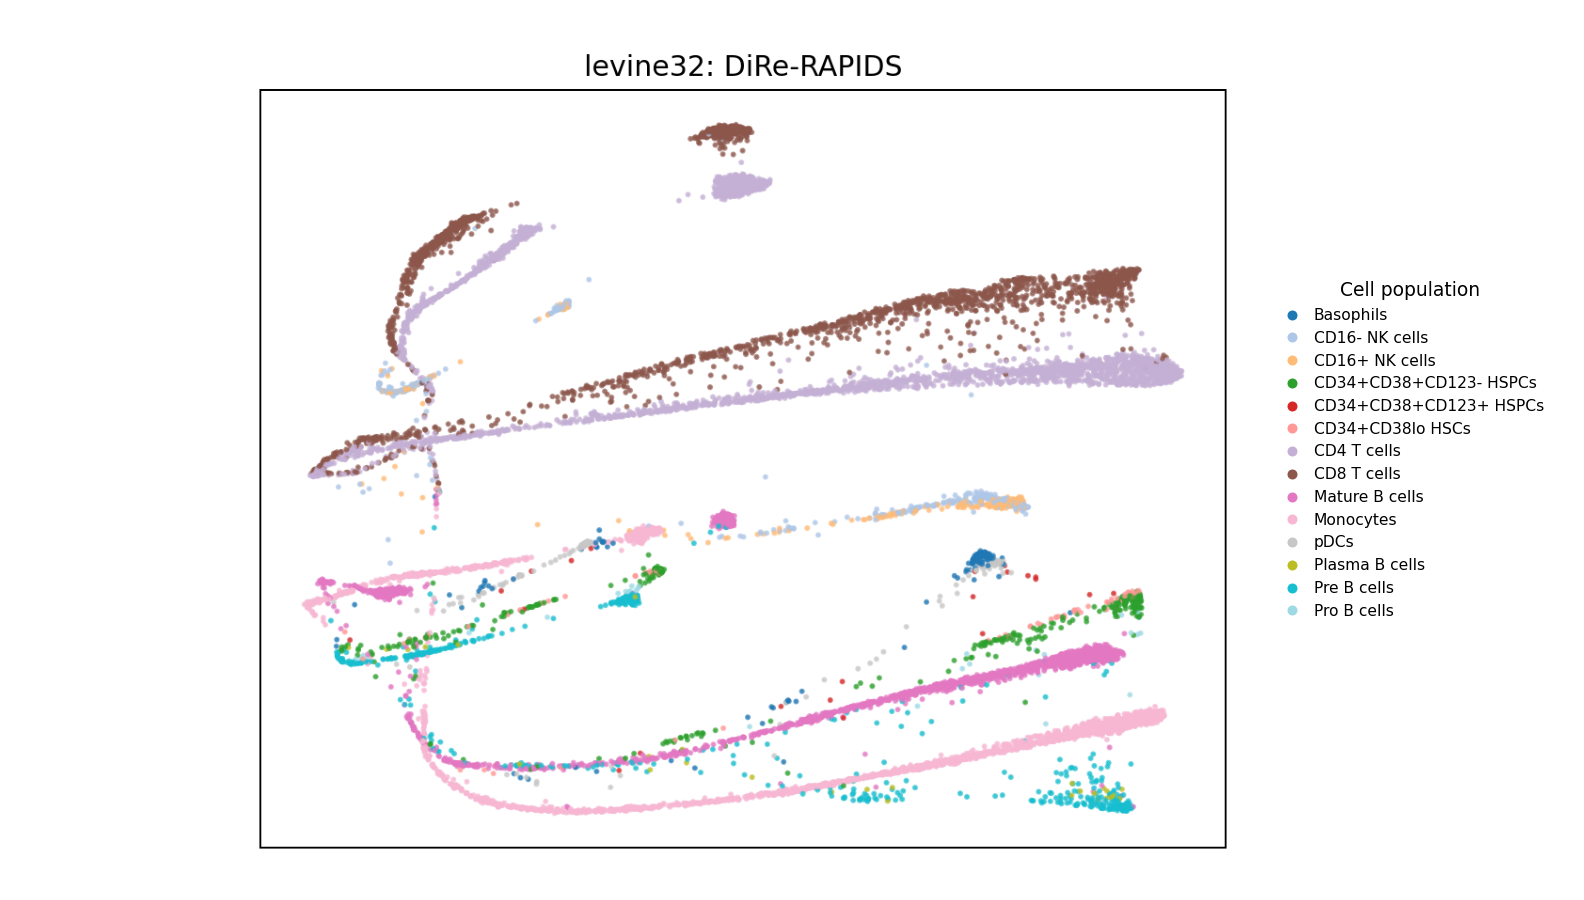
\includegraphics[width=\textwidth]{pics/embeddings/levine32-dire-rapids.png}
        \caption{DiRe--RAPIDS}
        \label{fig:lev32-dire-rapids}
    \end{subfigure}
    \hfill
    \begin{subfigure}[b]{0.45\textwidth}
        \centering
        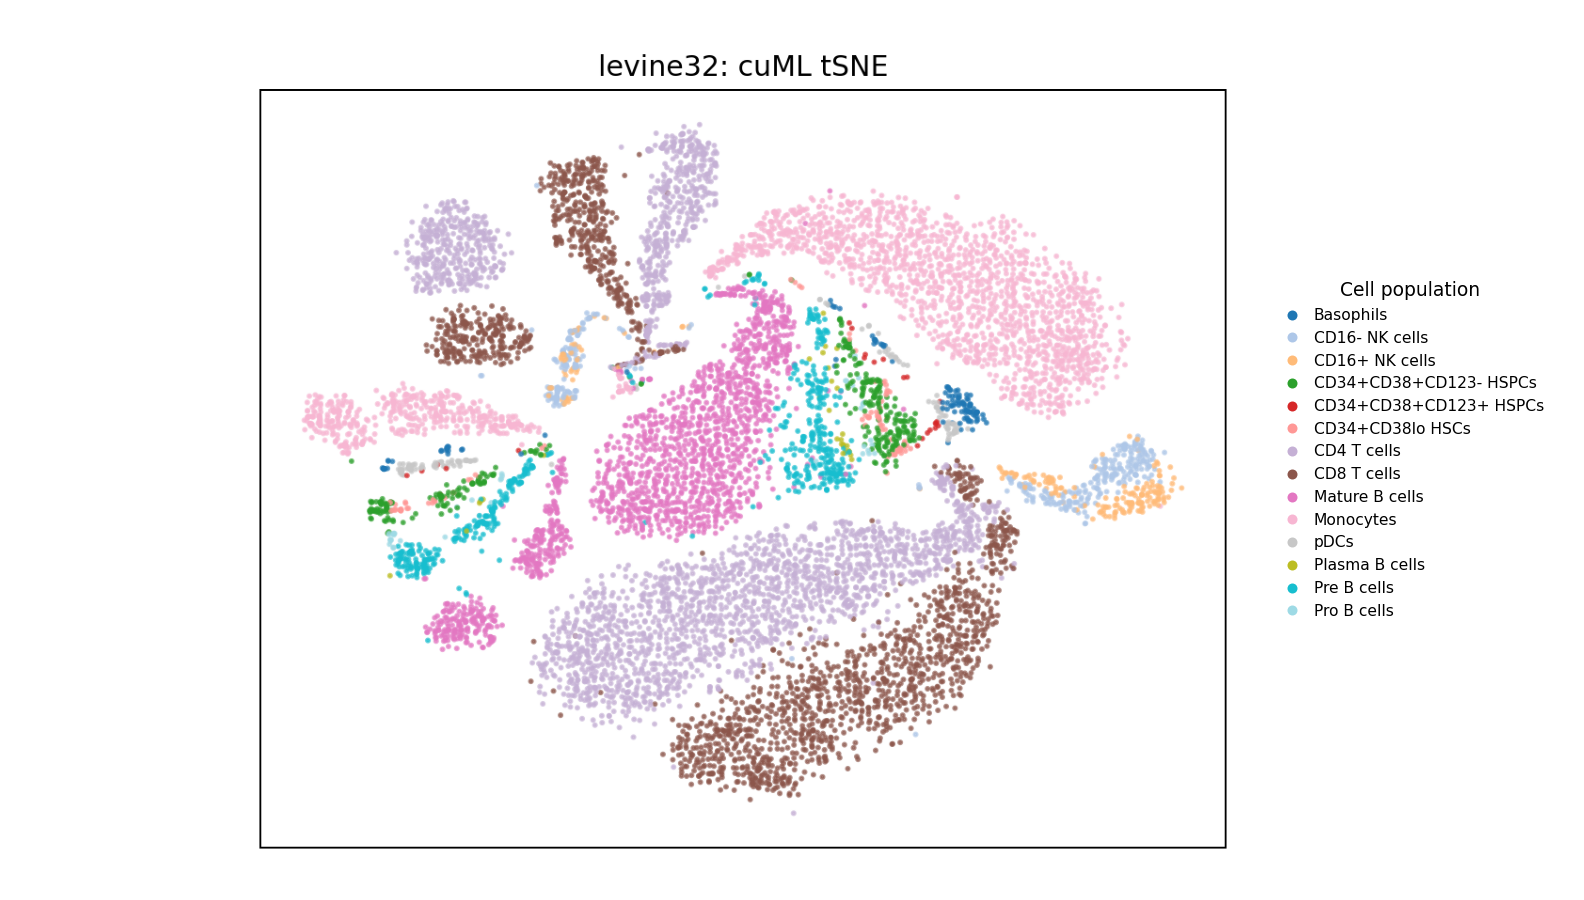
\includegraphics[width=\textwidth]{pics/embeddings/levine32-tsne.png}
        \caption{cuML tSNE}
        \label{fig:lev32-tsne}
    \end{subfigure}
    \vspace{1em}
    \begin{subfigure}[b]{0.45\textwidth}
        \centering
        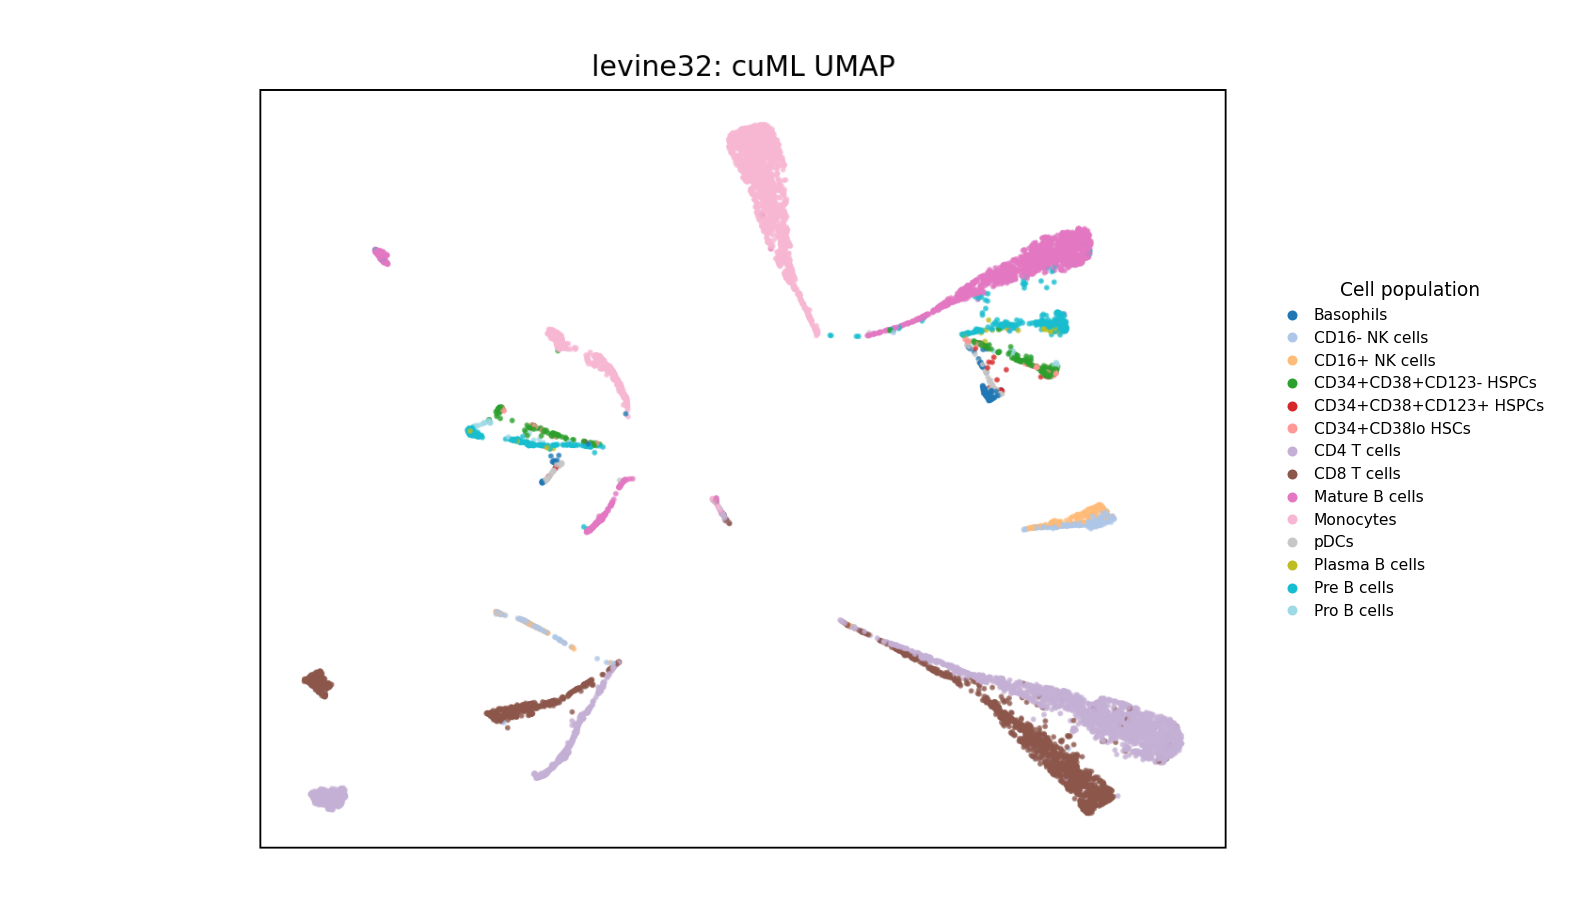
\includegraphics[width=\textwidth]{pics/embeddings/levine32-cuml-umap.png}
        \caption{cuML UMAP}
        \label{fig:lev32-cuml-umap}
    \end{subfigure}
    \hfill
    \begin{subfigure}[b]{0.45\textwidth}
        \centering
        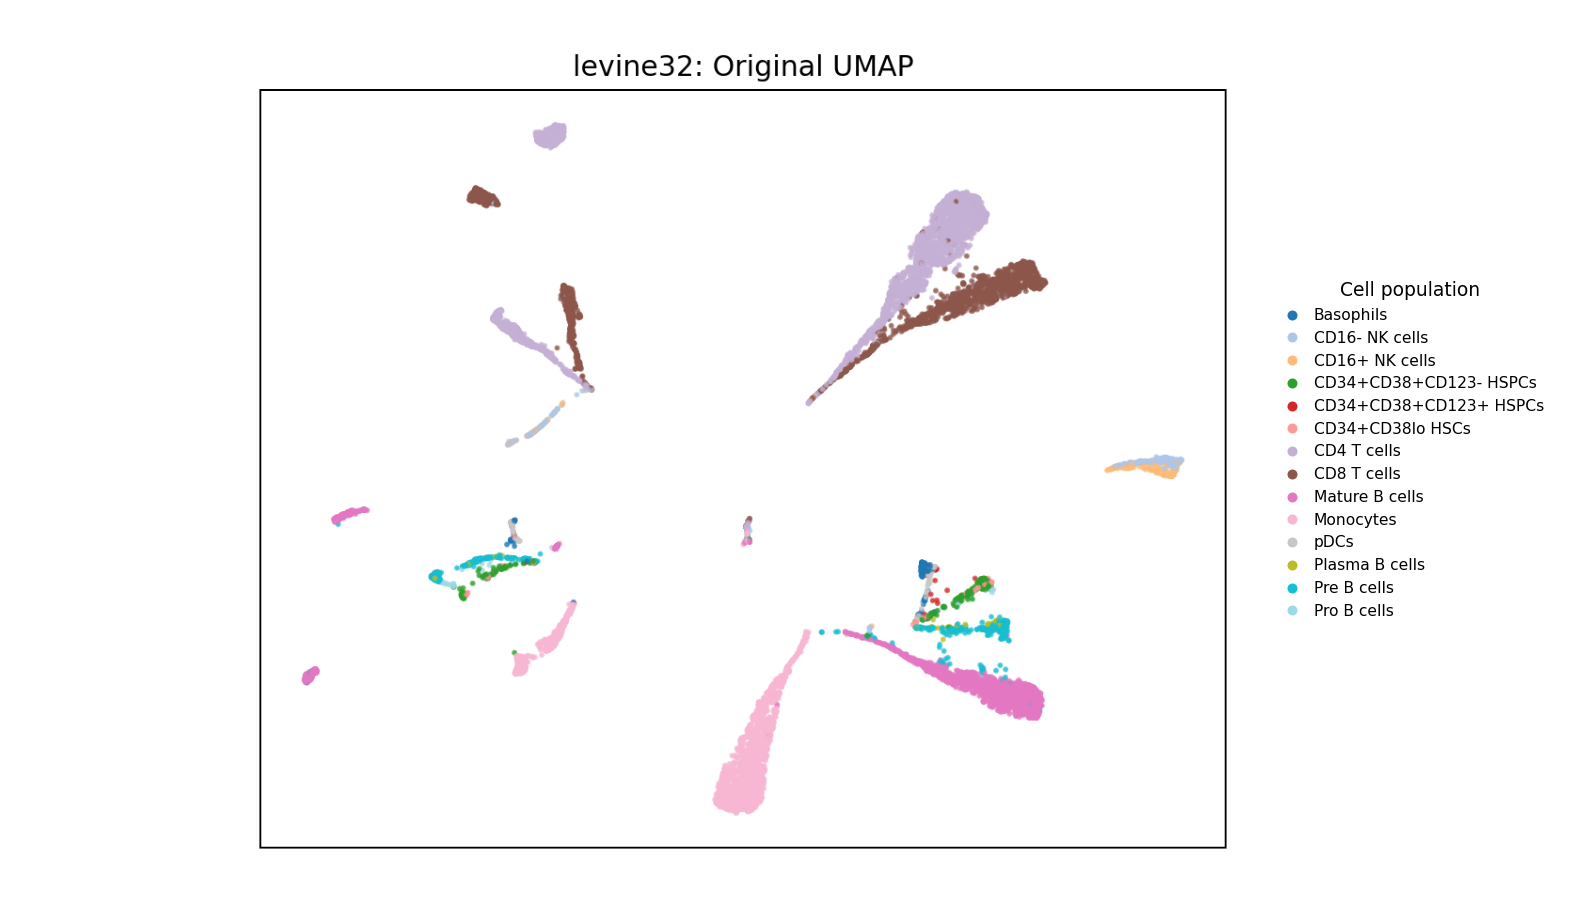
\includegraphics[width=\textwidth]{pics/embeddings/levine32-umap.png}
        \caption{Original UMAP}
        \label{fig:lev32-umap}
    \end{subfigure}
    \caption{"Levine 32" dataset embeddings}
    \label{fig:levine32}
\end{figure}

More benchmarking data is available in Appendix~\ref{appendix:levine32}. 

\section{Conclusions}

A new dimensionality reduction framework, called \texttt{DiRe}, has been developed with an explicit emphasis on preserving and measuring the dataset's homological structure. The latter is quantified by persistent homology and expressed via persistence diagrams or Betti curves. The benchmarks and metrics provided give evidence that DiRe can preserve global structure in cases where purely local criteria are insufficient, while also showing that no single metric captures every scientifically relevant aspect of an embedding.

The numerical experiments in this manuscript use DiRe--RAPIDS \cite{dire-rapids}; the earlier DiRe--JAX implementation remains available from GitHub \cite{dire-github} and is described in the JOSS publication \cite{dire-joss}.

The benchmark logs, archived embedding images, plotting scripts, manuscript build scripts, and Sphinx version of this manuscript are available in a separate reproducibility repository \cite{homological-stability-repro}. The DiRe implementation used by those scripts is DiRe--RAPIDS \cite{dire-rapids}. GPU acceleration is recommended for rerunning the largest datasets and for runtime comparisons against cuML baselines.

\section{Funding} This work is supported by the Google~Cloud Research Award number GCP19980904. The computational benchmarks were run in part on Lambda Labs GPU infrastructure; we thank Lambda Labs for supporting this work with access to GPU computing resources.

\section{Author Contributions} A.K. and I.R. developed the necessary theoretical background and main algorithm. A.K. produced and prepared figures. All authors reviewed the manuscript.

\newpage

\printbibliography

\newpage

\section{Blobs: Dataset Metrics}\label{appendix:blobs}

\begin{figure}[ht]
    \centering
    \begin{subfigure}[b]{0.35\textwidth}
        \centering
        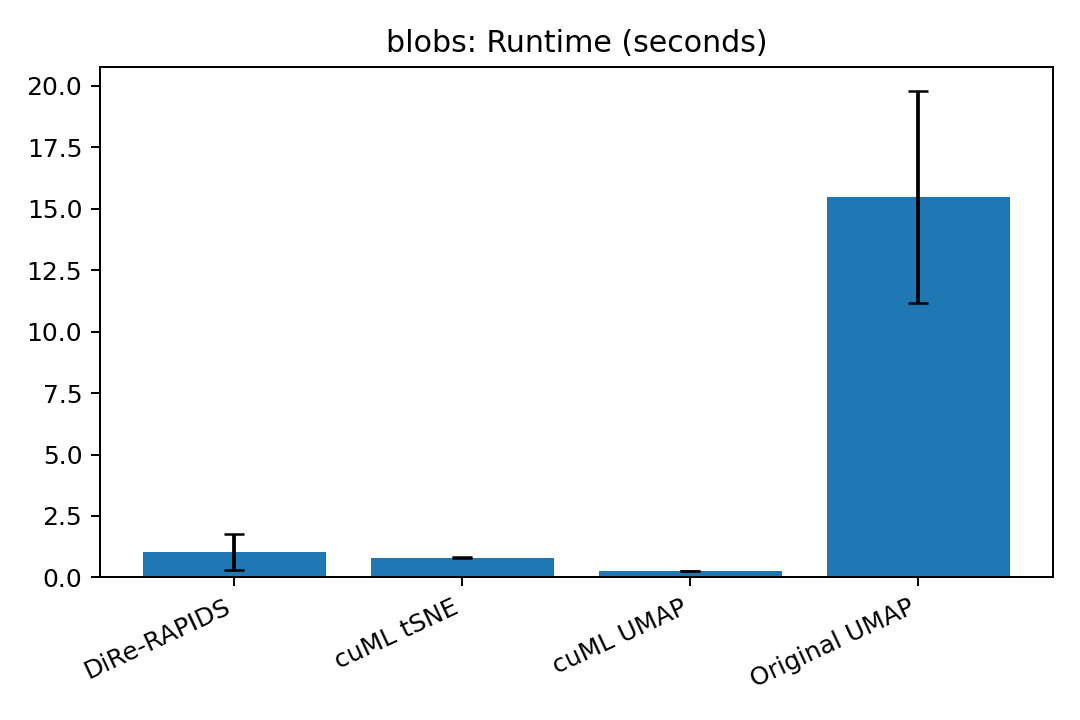
\includegraphics[width=\textwidth]{pics/blobs_comparison/blobs-time.png}
        \caption{Runtime (seconds)}
        \label{fig:blobs-time}
    \end{subfigure}
    \hfill
    \begin{subfigure}[b]{0.35\textwidth}
        \centering
        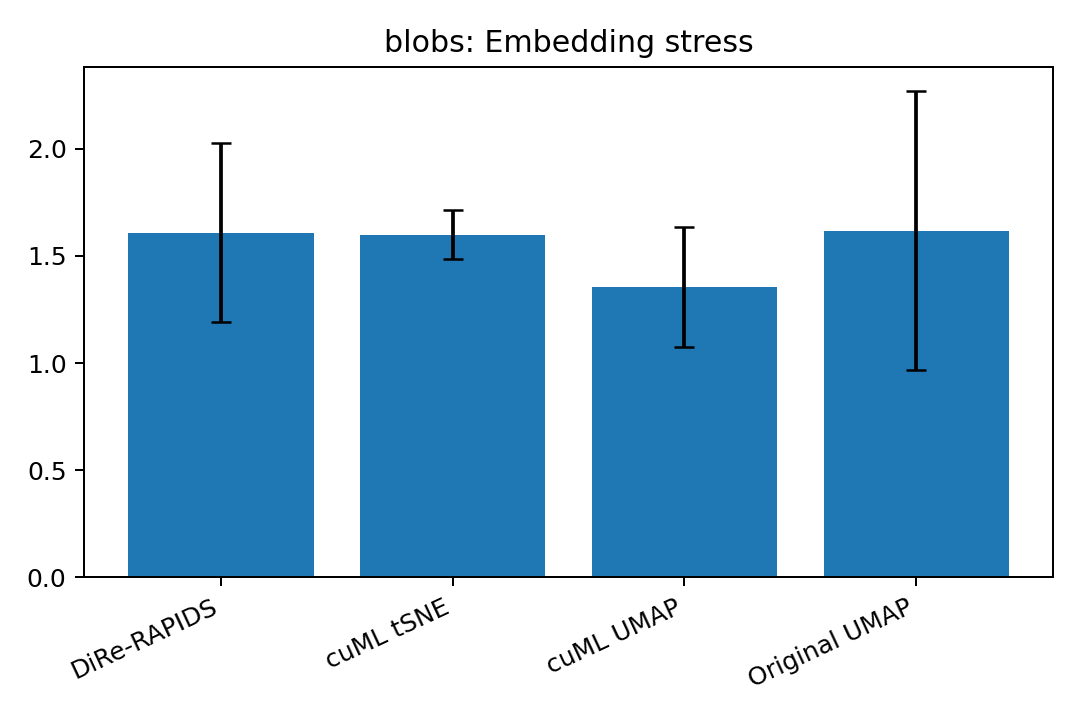
\includegraphics[width=\textwidth]{pics/blobs_comparison/blobs-stress.png}
        \caption{Embedding stress}
        \label{fig:blobs-stress}
    \end{subfigure}
    \vspace{1em}
    \begin{subfigure}[b]{0.35\textwidth}
        \centering
        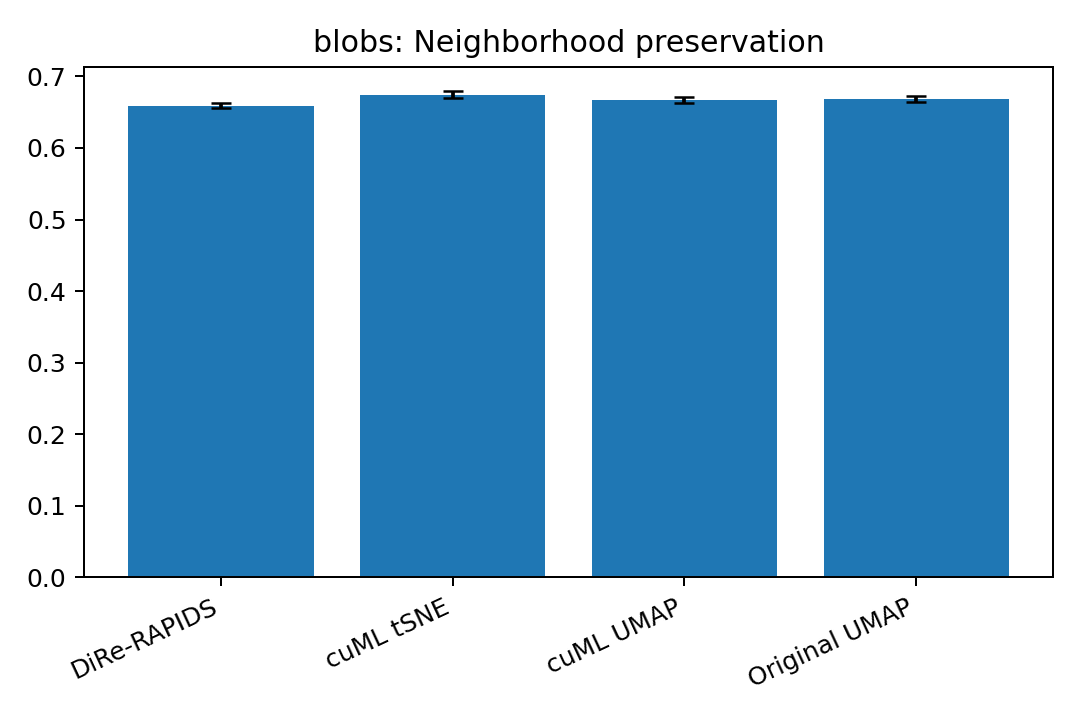
\includegraphics[width=\textwidth]{pics/blobs_comparison/blobs-neighborhood.png}
        \caption{Neighborhood preservation}
        \label{fig:blobs-neighborhood}
    \end{subfigure}
    \hfill
    \begin{subfigure}[b]{0.35\textwidth}
        \centering
        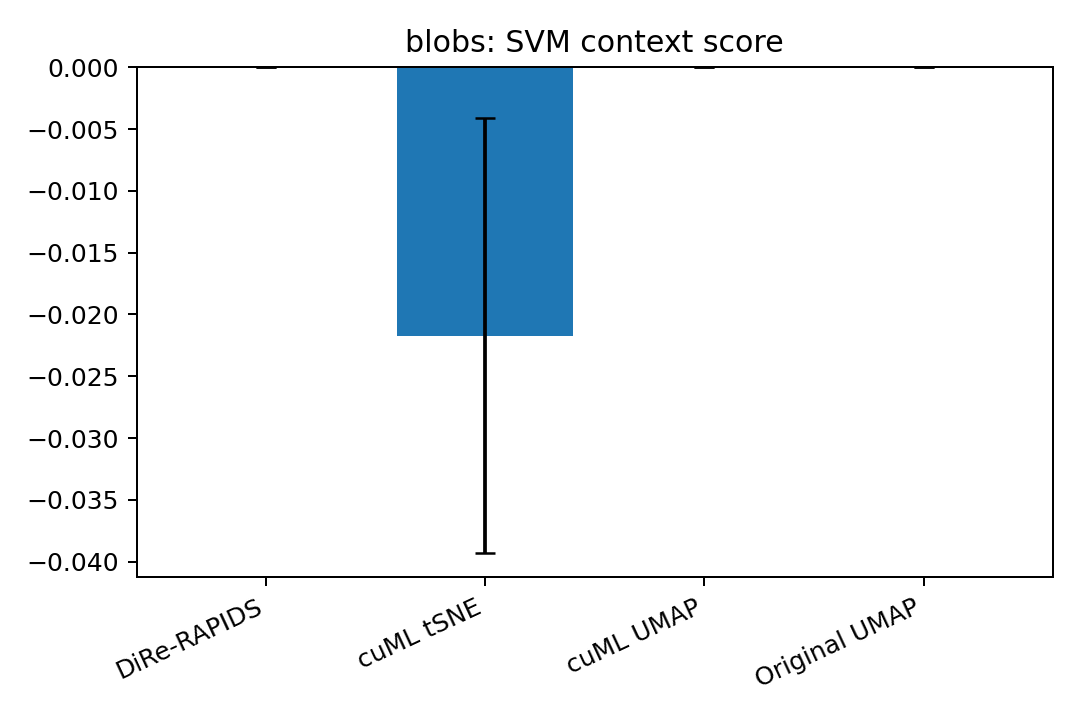
\includegraphics[width=\textwidth]{pics/blobs_comparison/blobs-context.png}
        \caption{SVM context score}
        \label{fig:blobs-context}
    \end{subfigure}
    \hfill
    \begin{subfigure}[b]{0.35\textwidth}
        \centering
        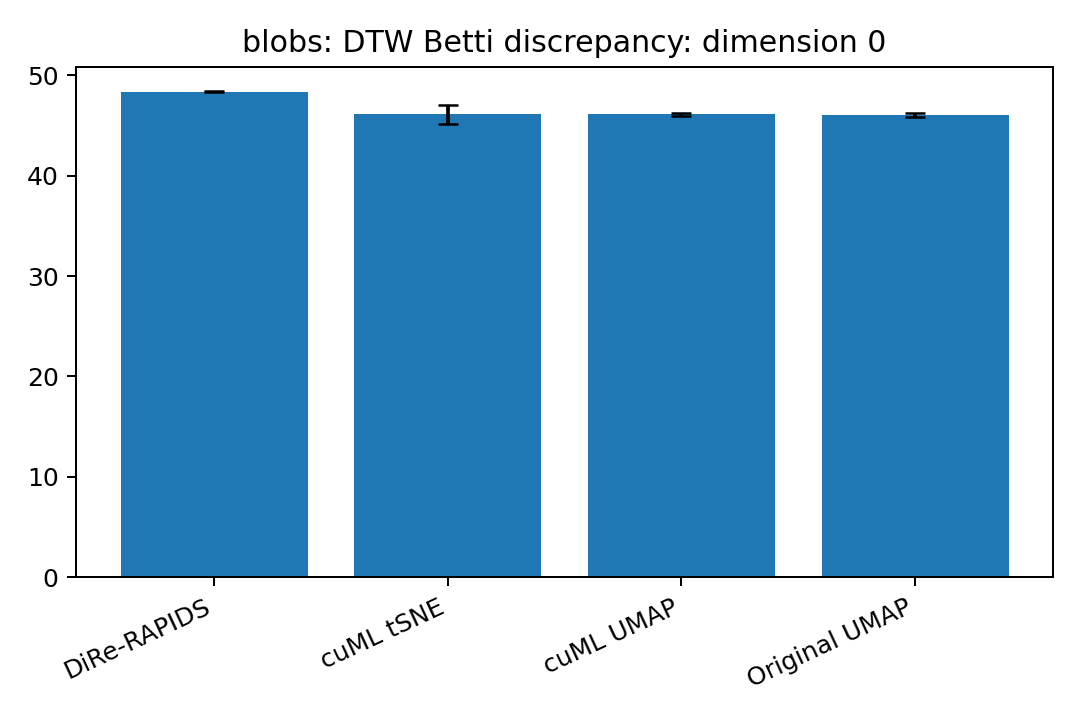
\includegraphics[width=\textwidth]{pics/blobs_comparison/blobs-persistence-dim-0.png}
        \caption{DTW Betti discrepancy: dimension $0$}
        \label{fig:blobs-persistence-0}
    \end{subfigure}
    \hfill
    \begin{subfigure}[b]{0.35\textwidth}
        \centering
        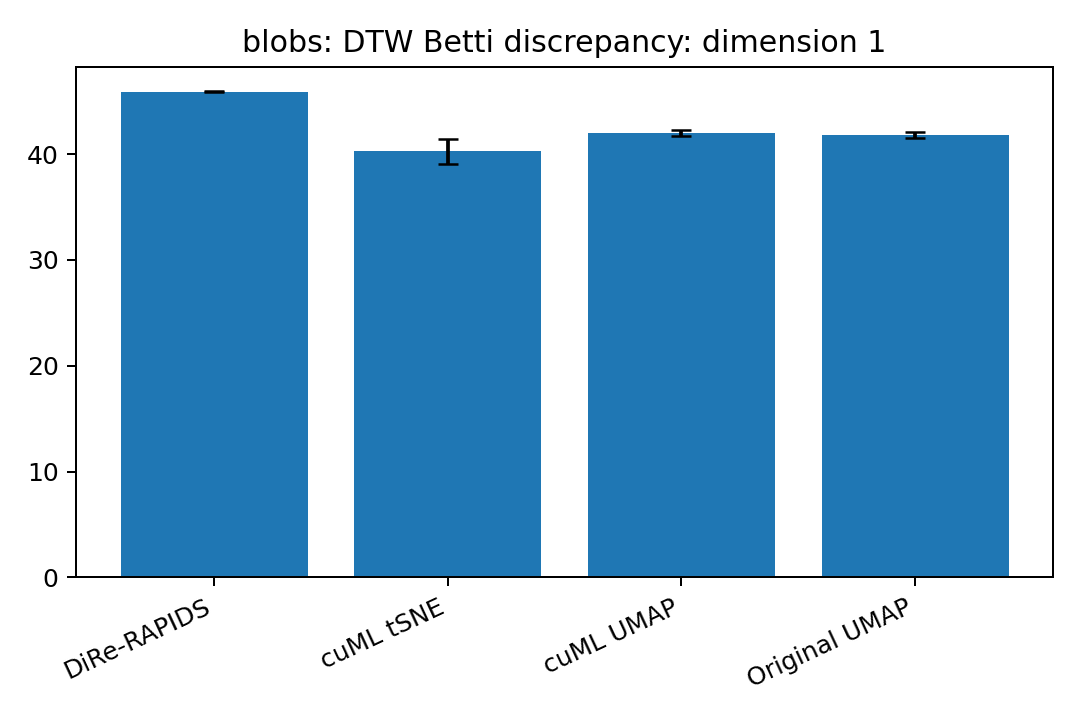
\includegraphics[width=\textwidth]{pics/blobs_comparison/blobs-persistence-dim-1.png}
        \caption{DTW Betti discrepancy: dimension $1$}
        \label{fig:blobs-persistence-1}
    \end{subfigure}
    \caption{"Blobs" dataset metrics comparison. Error bars show sample standard deviations.}
    \label{fig:blobs-comparison}
\end{figure}

\newpage

\section{MNIST Digits: Dataset Metrics}\label{appendix:mnist}

\begin{figure}[ht]
    \centering
    \begin{subfigure}[b]{0.35\textwidth}
        \centering
        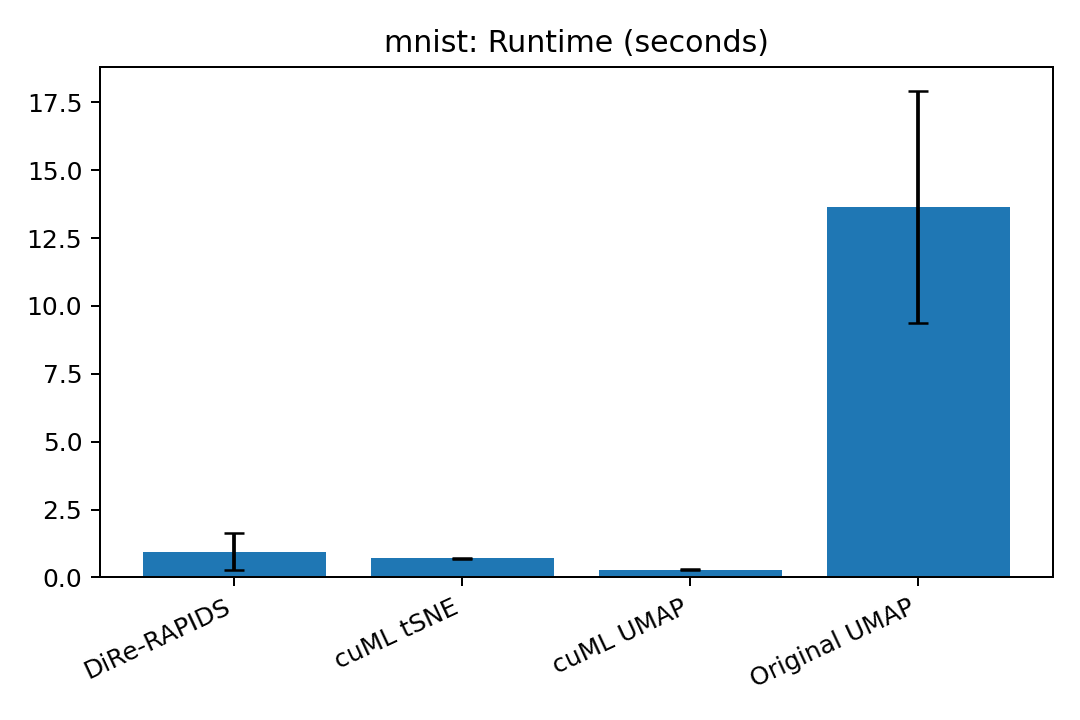
\includegraphics[width=\textwidth]{pics/mnist_comparison/mnist-time.png}
        \caption{Runtime (seconds)}
        \label{fig:mnist-time}
    \end{subfigure}
    \hfill
    \begin{subfigure}[b]{0.35\textwidth}
        \centering
        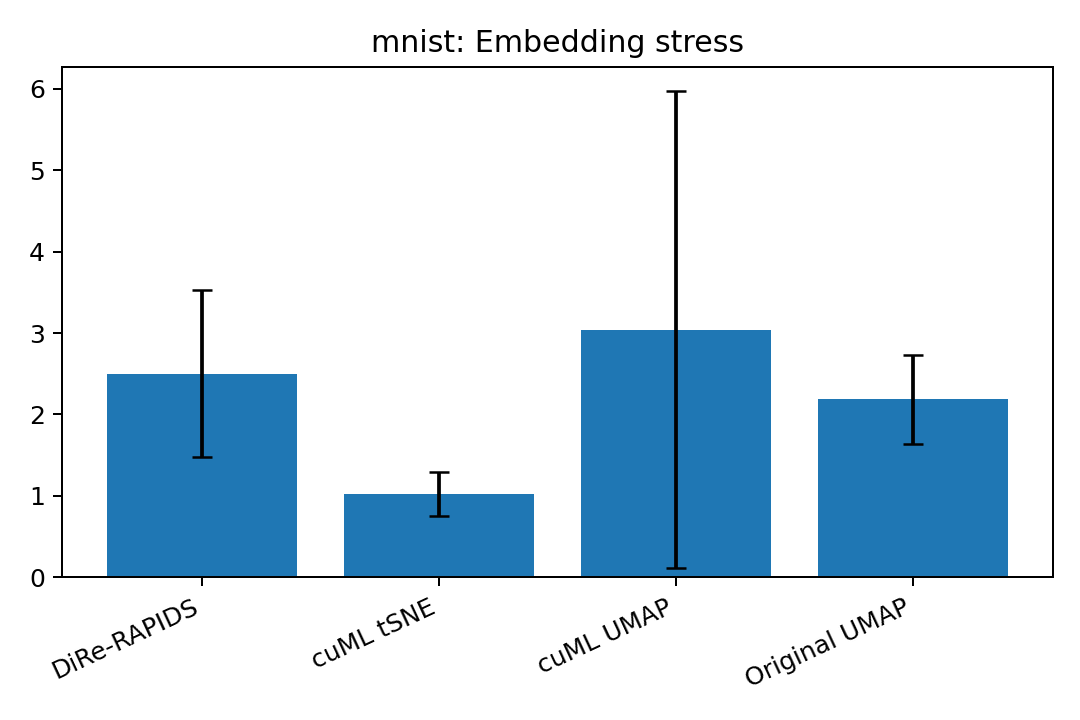
\includegraphics[width=\textwidth]{pics/mnist_comparison/mnist-stress.png}
        \caption{Embedding stress}
        \label{fig:mnist-stress}
    \end{subfigure}
    \vspace{1em}
    \begin{subfigure}[b]{0.35\textwidth}
        \centering
        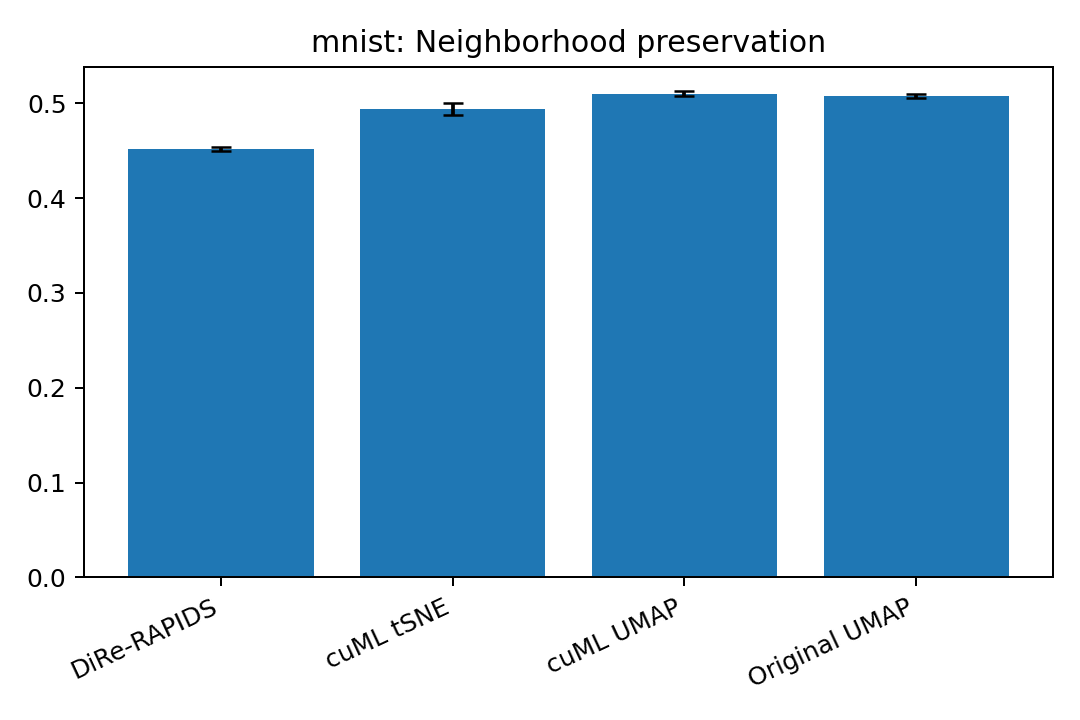
\includegraphics[width=\textwidth]{pics/mnist_comparison/mnist-neighborhood.png}
        \caption{Neighborhood preservation}
        \label{fig:mnist-neighborhood}
    \end{subfigure}
    \hfill
    \begin{subfigure}[b]{0.35\textwidth}
        \centering
        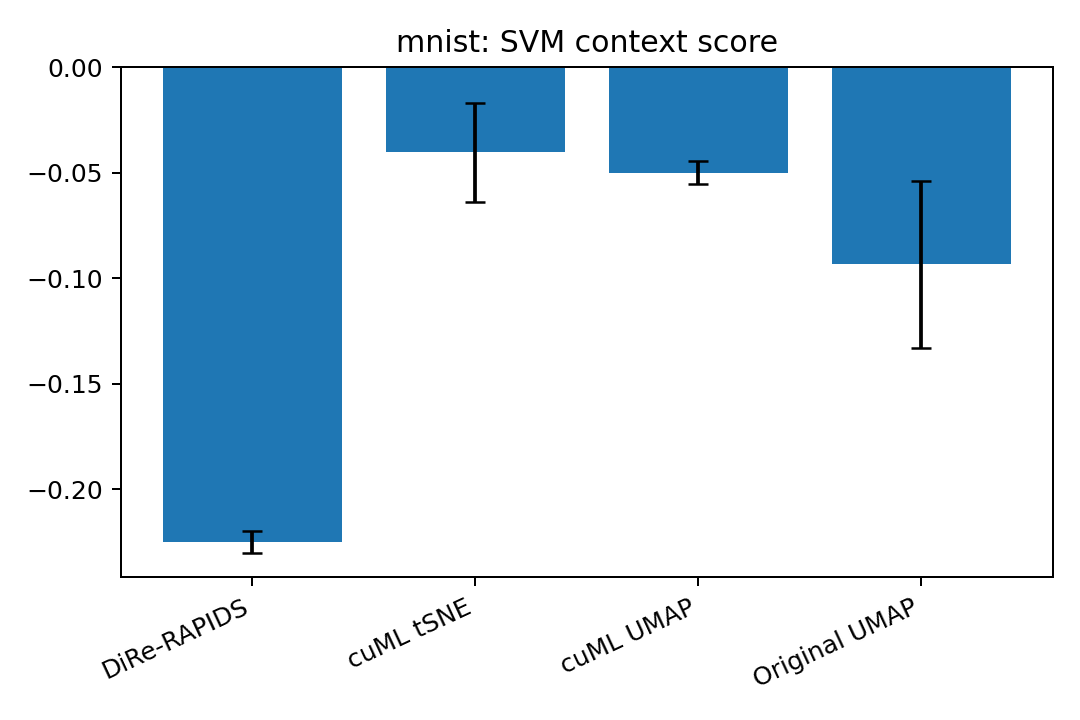
\includegraphics[width=\textwidth]{pics/mnist_comparison/mnist-context.png}
        \caption{SVM context score}
        \label{fig:mnist-context}
    \end{subfigure}
    \hfill
    \begin{subfigure}[b]{0.35\textwidth}
        \centering
        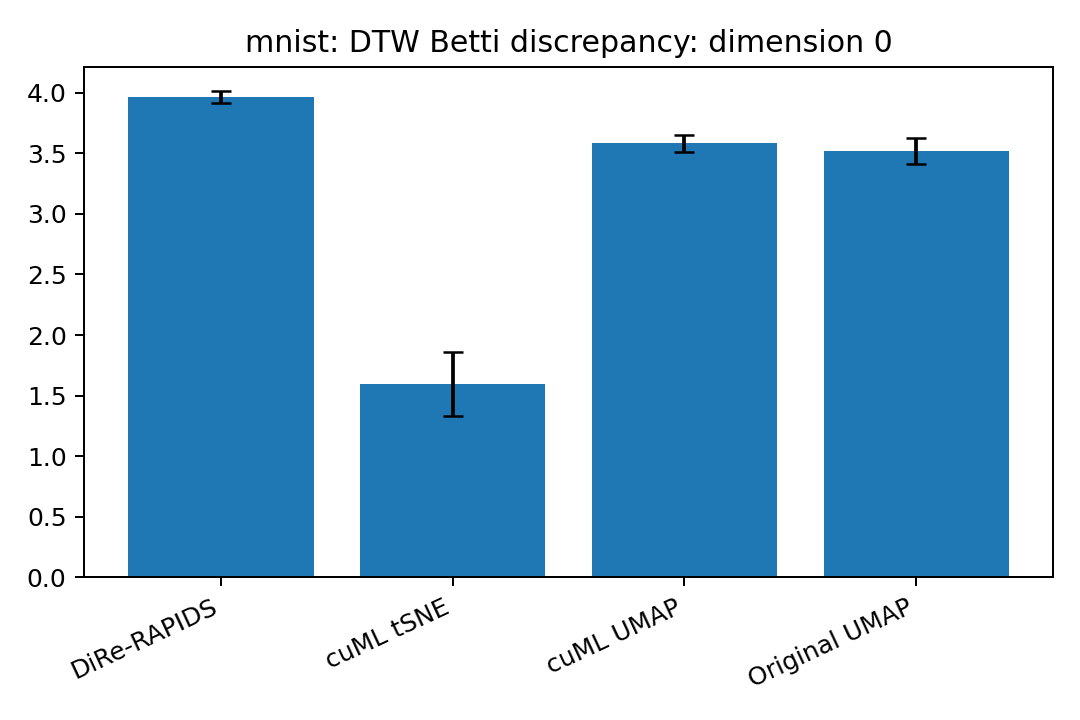
\includegraphics[width=\textwidth]{pics/mnist_comparison/mnist-persistence-dim-0.png}
        \caption{DTW Betti discrepancy: dimension $0$}
        \label{fig:mnist-persistence-0}
    \end{subfigure}
    \hfill
    \begin{subfigure}[b]{0.35\textwidth}
        \centering
        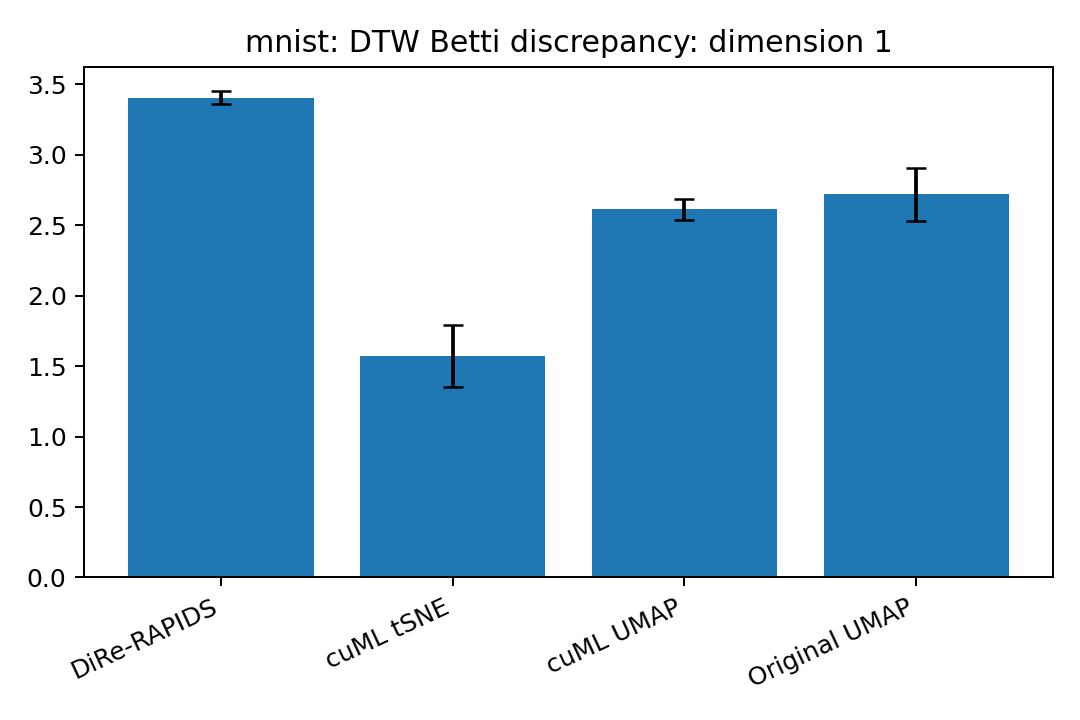
\includegraphics[width=\textwidth]{pics/mnist_comparison/mnist-persistence-dim-1.png}
        \caption{DTW Betti discrepancy: dimension $1$}
        \label{fig:mnist-persistence-1}
    \end{subfigure}
    \caption{"MNIST Digits" dataset metrics comparison. Error bars show sample standard deviations.}
    \label{fig:mnist-comparison}
\end{figure}

\newpage

\section{Disk Uniform: Dataset Metrics}\label{appendix:disk}

\begin{figure}[ht]
    \centering
    \begin{subfigure}[b]{0.35\textwidth}
        \centering
        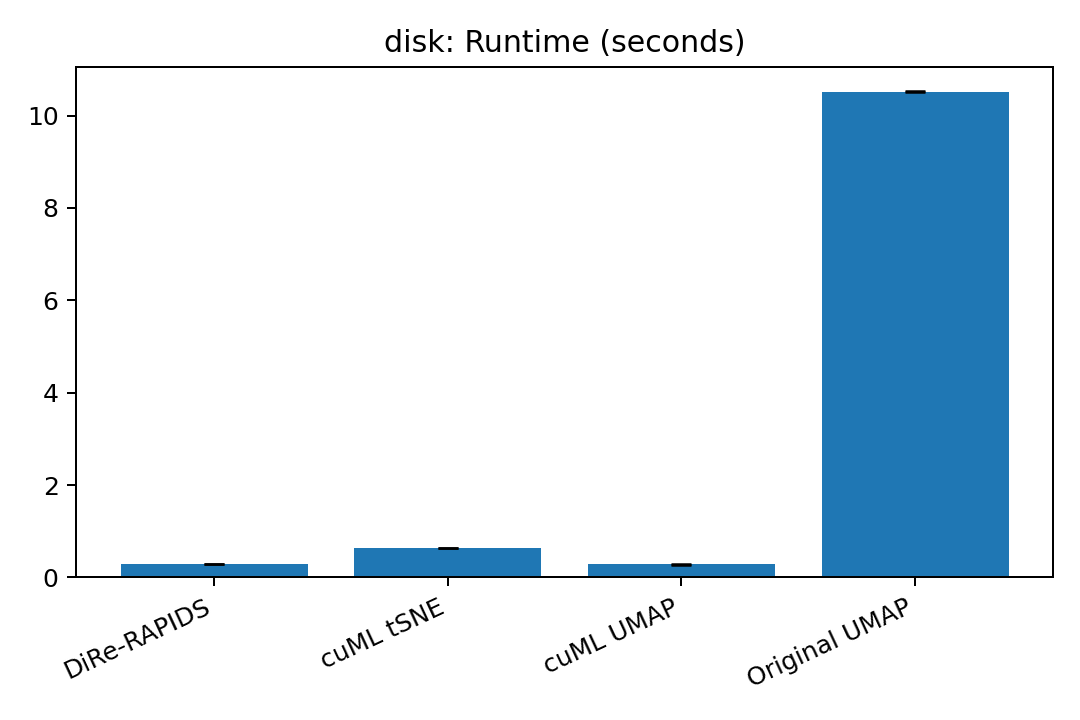
\includegraphics[width=\textwidth]{pics/disk_comparison/disk-time.png}
        \caption{Runtime (seconds)}
        \label{fig:disk-time}
    \end{subfigure}
    \hfill
    \begin{subfigure}[b]{0.35\textwidth}
        \centering
        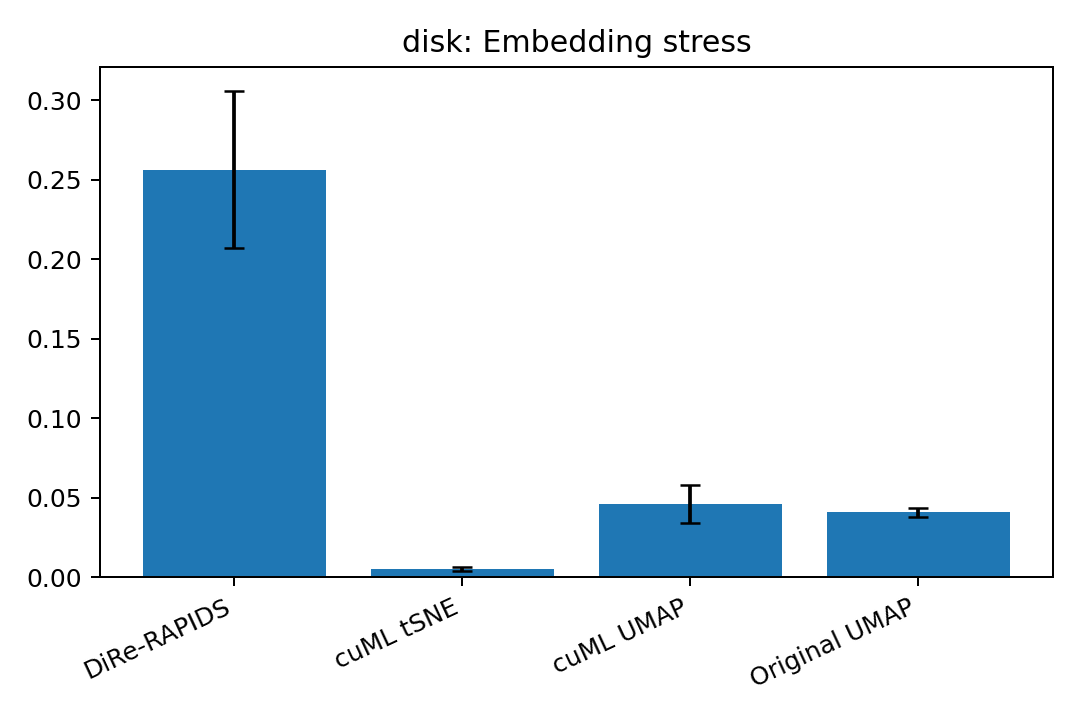
\includegraphics[width=\textwidth]{pics/disk_comparison/disk-stress.png}
        \caption{Embedding stress}
        \label{fig:disk-stress}
    \end{subfigure}
    \vspace{1em}
    \begin{subfigure}[b]{0.35\textwidth}
        \centering
        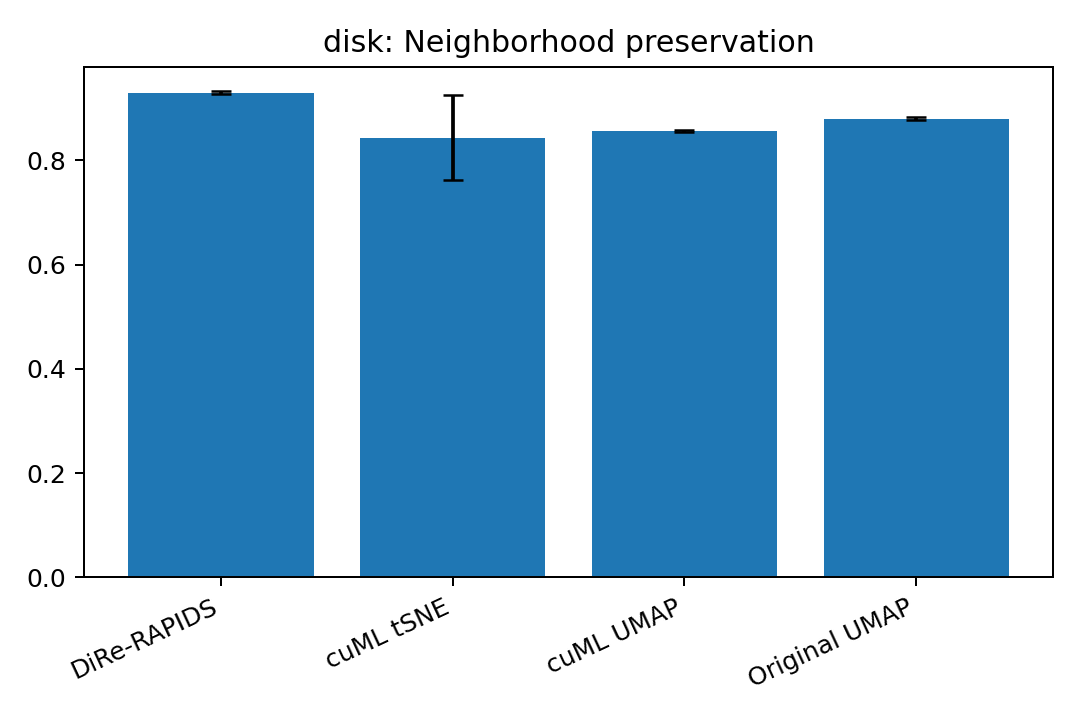
\includegraphics[width=\textwidth]{pics/disk_comparison/disk-neighborhood.png}
        \caption{Neighborhood preservation}
        \label{fig:disk-neighborhood}
    \end{subfigure}
    \hfill
    \begin{subfigure}[b]{0.35\textwidth}
        \centering
        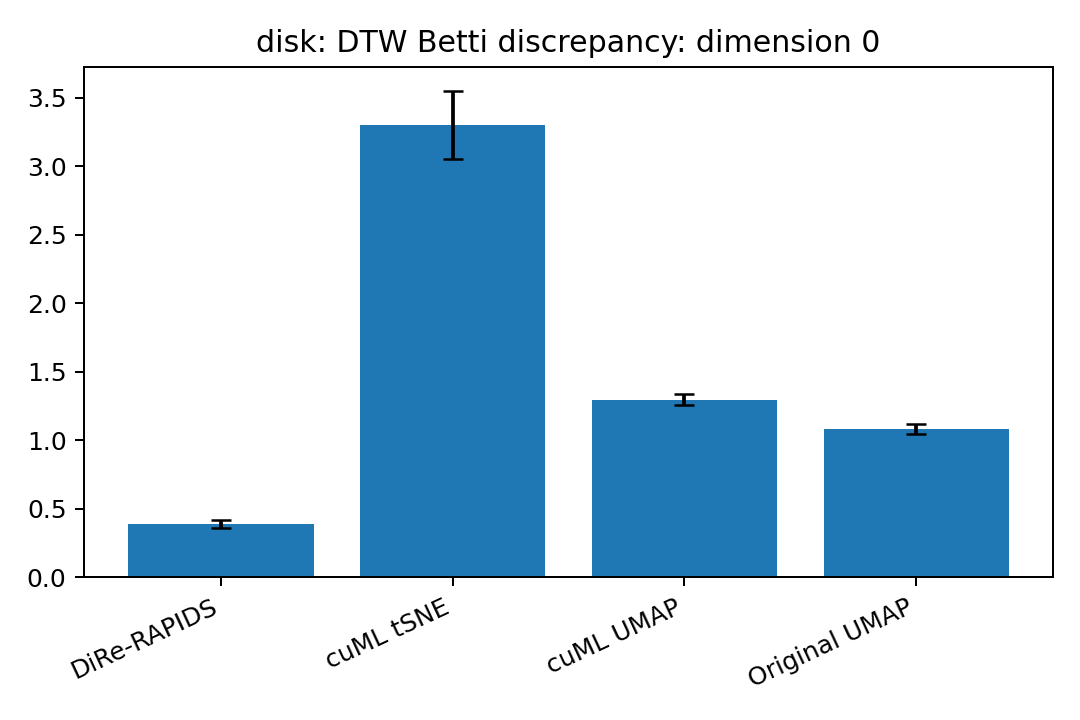
\includegraphics[width=\textwidth]{pics/disk_comparison/disk-persistence-dim-0.png}
        \caption{DTW Betti discrepancy: dimension $0$}
        \label{fig:disk-persistence-0}
    \end{subfigure}
    \hfill
    \begin{subfigure}[b]{0.35\textwidth}
        \centering
        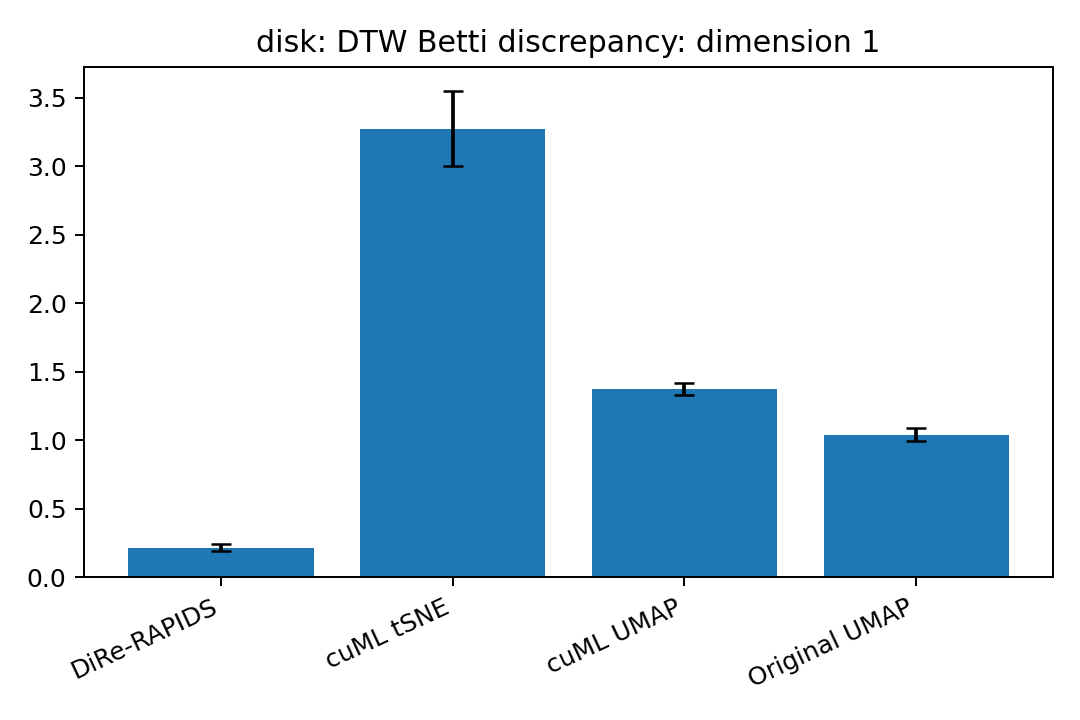
\includegraphics[width=\textwidth]{pics/disk_comparison/disk-persistence-dim-1.png}
        \caption{DTW Betti discrepancy: dimension $1$}
        \label{fig:disk-persistence-1}
    \end{subfigure}
    \caption{"Disk Uniform" dataset metrics comparison. Error bars show sample standard deviations.}
    \label{fig:disk-comparison}
\end{figure}

\newpage

\section{Half--moons: Dataset Metrics}\label{appendix:moons}


\begin{figure}[ht]
    \centering
    \begin{subfigure}[b]{0.35\textwidth}
        \centering
        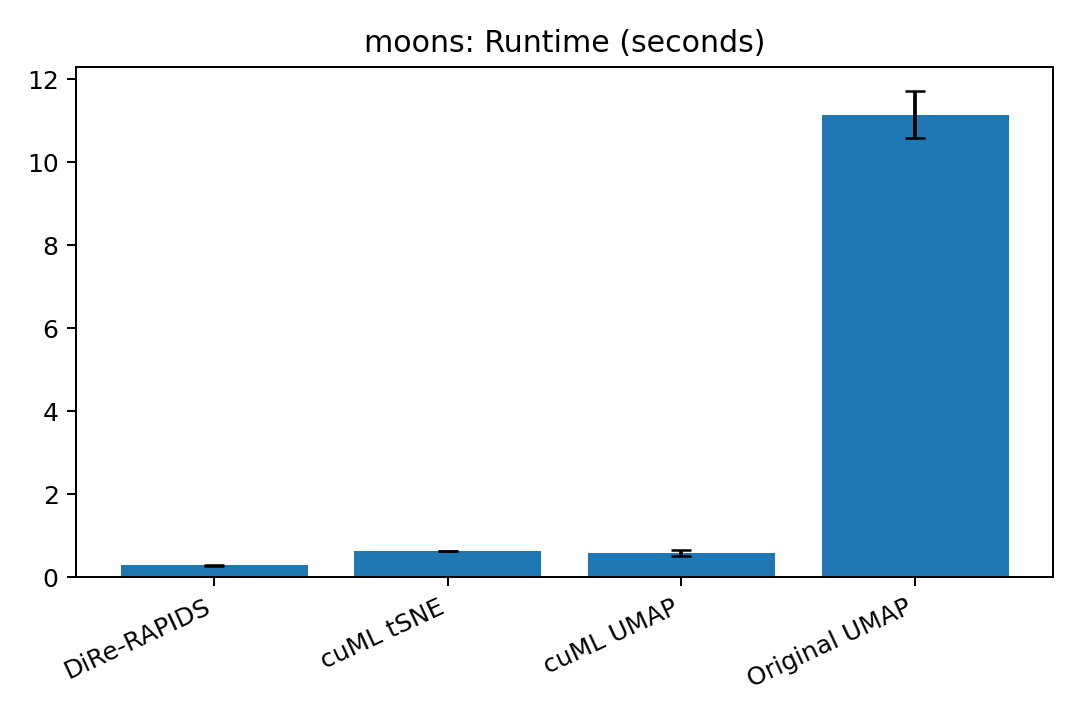
\includegraphics[width=\textwidth]{pics/moons_comparison/moons-time.png}
        \caption{Runtime (seconds)}
        \label{fig:moons-time}
    \end{subfigure}
    \hfill
    \begin{subfigure}[b]{0.35\textwidth}
        \centering
        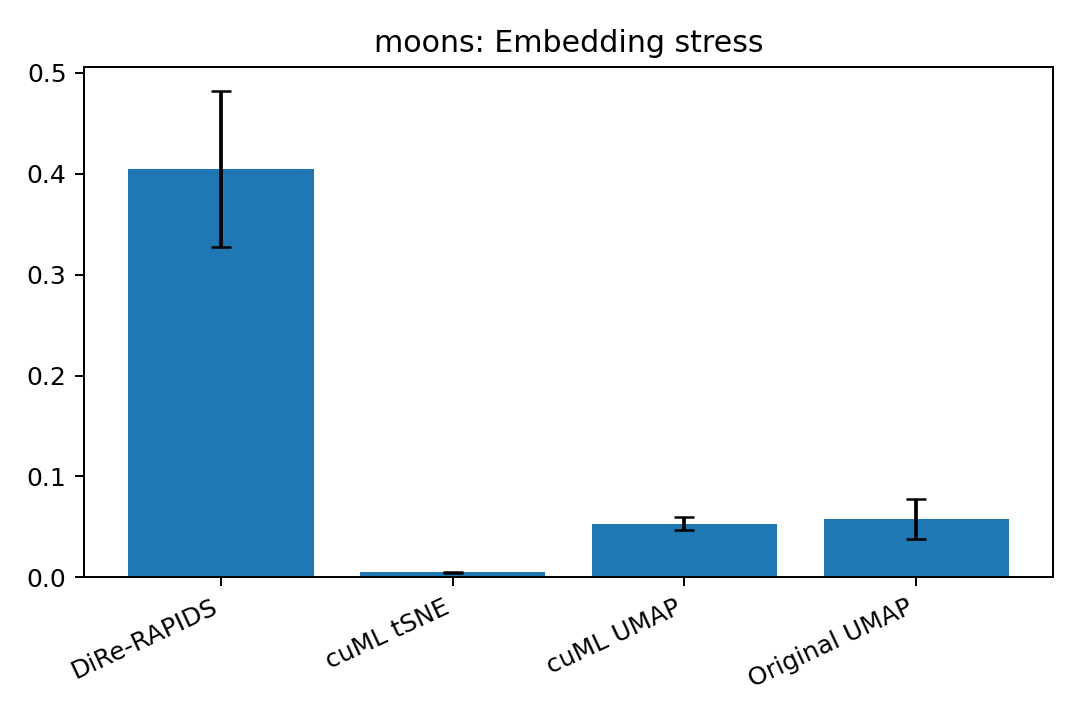
\includegraphics[width=\textwidth]{pics/moons_comparison/moons-stress.png}
        \caption{Embedding stress}
        \label{fig:moons-stress}
    \end{subfigure}
    \vspace{1em}
    \begin{subfigure}[b]{0.35\textwidth}
        \centering
        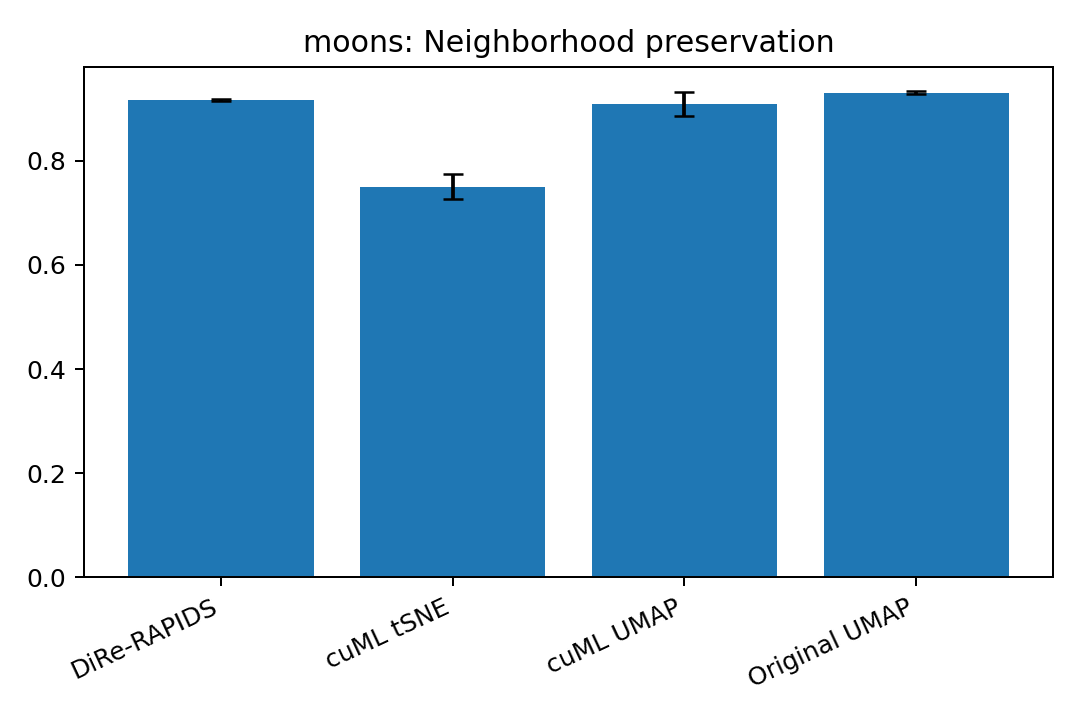
\includegraphics[width=\textwidth]{pics/moons_comparison/moons-neighborhood.png}
        \caption{Neighborhood preservation}
        \label{fig:moons-neighborhood}
    \end{subfigure}
    \hfill
    \begin{subfigure}[b]{0.35\textwidth}
        \centering
        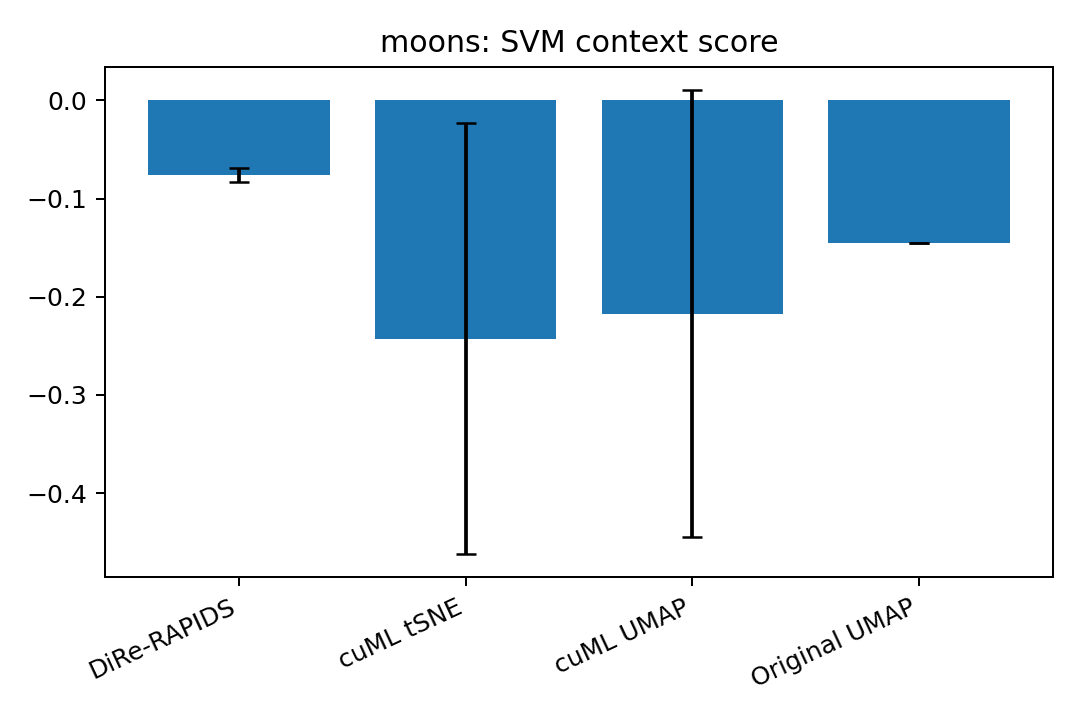
\includegraphics[width=\textwidth]{pics/moons_comparison/moons-context.png}
        \caption{SVM context score}
        \label{fig:moons-context}
    \end{subfigure}
    \hfill
    \begin{subfigure}[b]{0.35\textwidth}
        \centering
        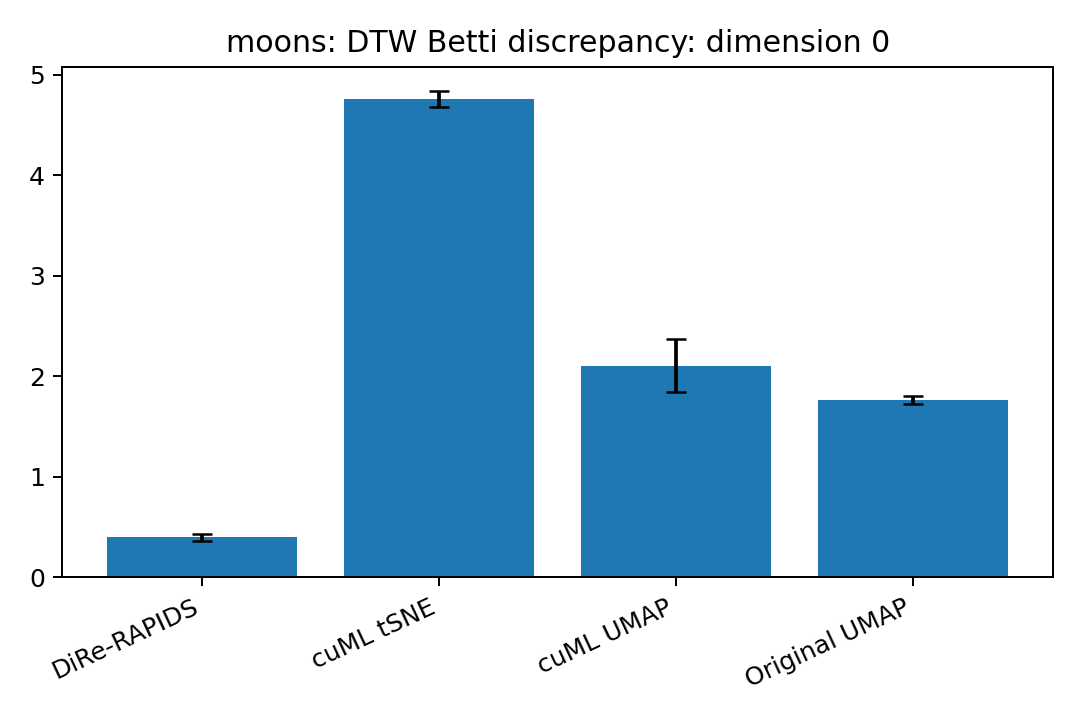
\includegraphics[width=\textwidth]{pics/moons_comparison/moons-persistence-dim-0.png}
        \caption{DTW Betti discrepancy: dimension $0$}
        \label{fig:moons-persistence-0}
    \end{subfigure}
    \hfill
    \begin{subfigure}[b]{0.35\textwidth}
        \centering
        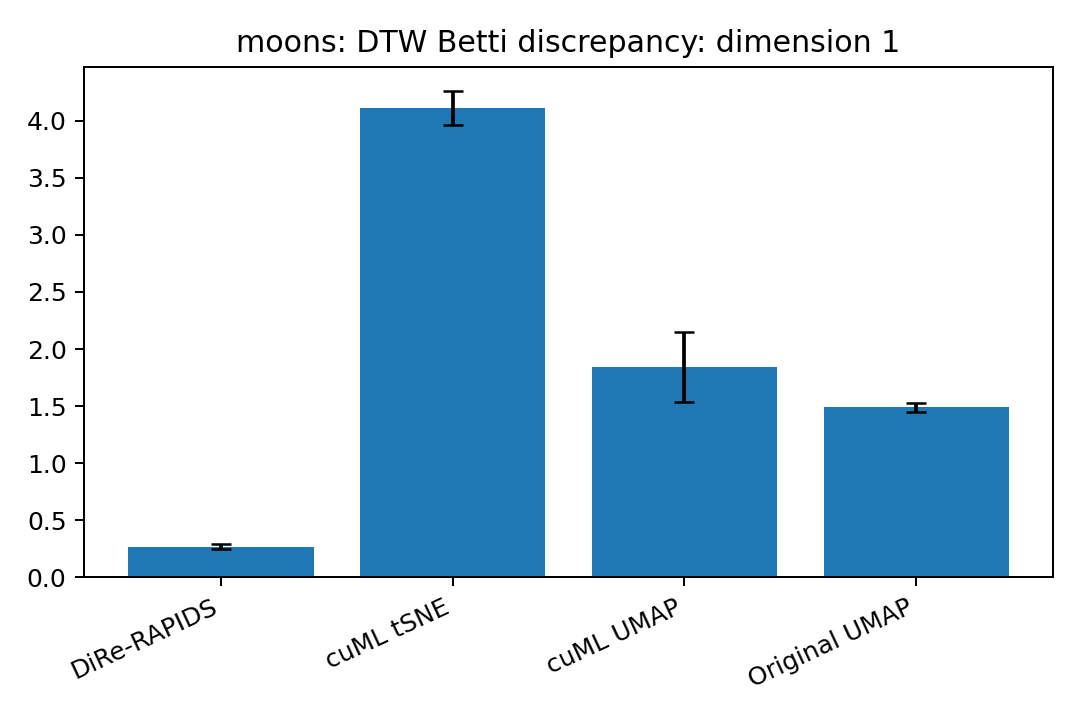
\includegraphics[width=\textwidth]{pics/moons_comparison/moons-persistence-dim-1.png}
        \caption{DTW Betti discrepancy: dimension $1$}
        \label{fig:moons-persistence-1}
    \end{subfigure}
    \caption{"Half--moons" dataset metrics comparison. Error bars show sample standard deviations.}
    \label{fig:moons-comparison}
\end{figure}

\newpage

\section{Levine 13: Dataset Metrics}\label{appendix:levine13}



\begin{figure}[ht]
    \centering
    \begin{subfigure}[b]{0.35\textwidth}
        \centering
        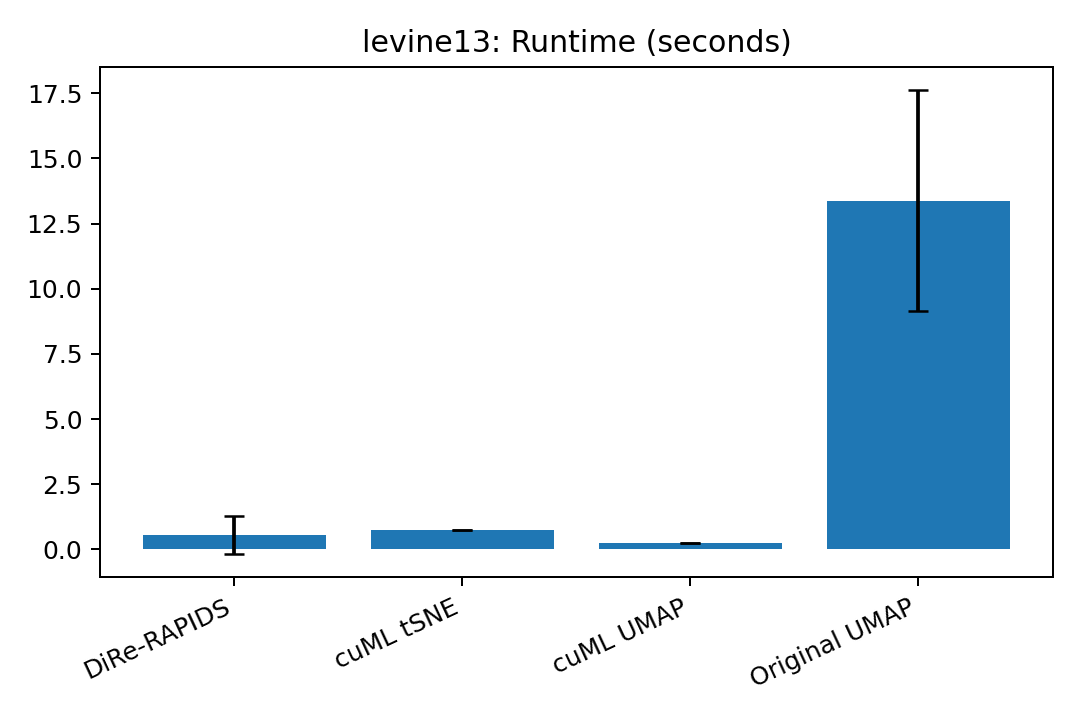
\includegraphics[width=\textwidth]{pics/levine13_comparison/levine13-time.png}
        \caption{Runtime (seconds)}
        \label{fig:levine13-time}
    \end{subfigure}
    \hfill
    \begin{subfigure}[b]{0.35\textwidth}
        \centering
        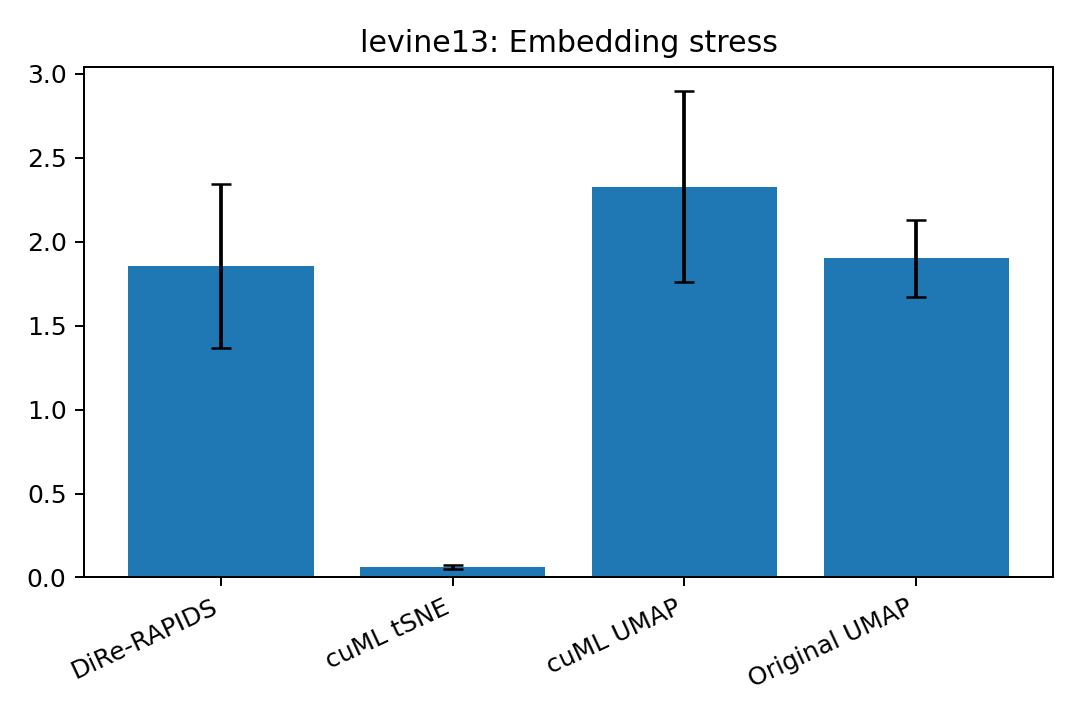
\includegraphics[width=\textwidth]{pics/levine13_comparison/levine13-stress.png}
        \caption{Embedding stress}
        \label{fig:levine13-stress}
    \end{subfigure}
    \vspace{1em}
    \begin{subfigure}[b]{0.35\textwidth}
        \centering
        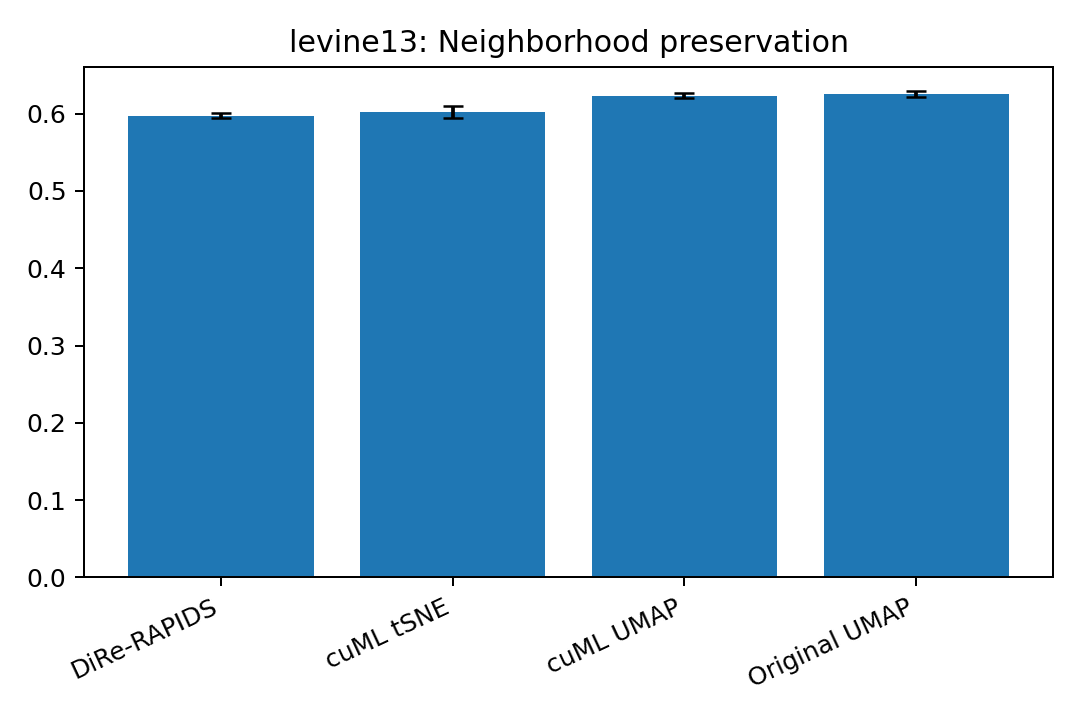
\includegraphics[width=\textwidth]{pics/levine13_comparison/levine13-neighborhood.png}
        \caption{Neighborhood preservation}
        \label{fig:levine13-neighborhood}
    \end{subfigure}
    \hfill
    \begin{subfigure}[b]{0.35\textwidth}
        \centering
        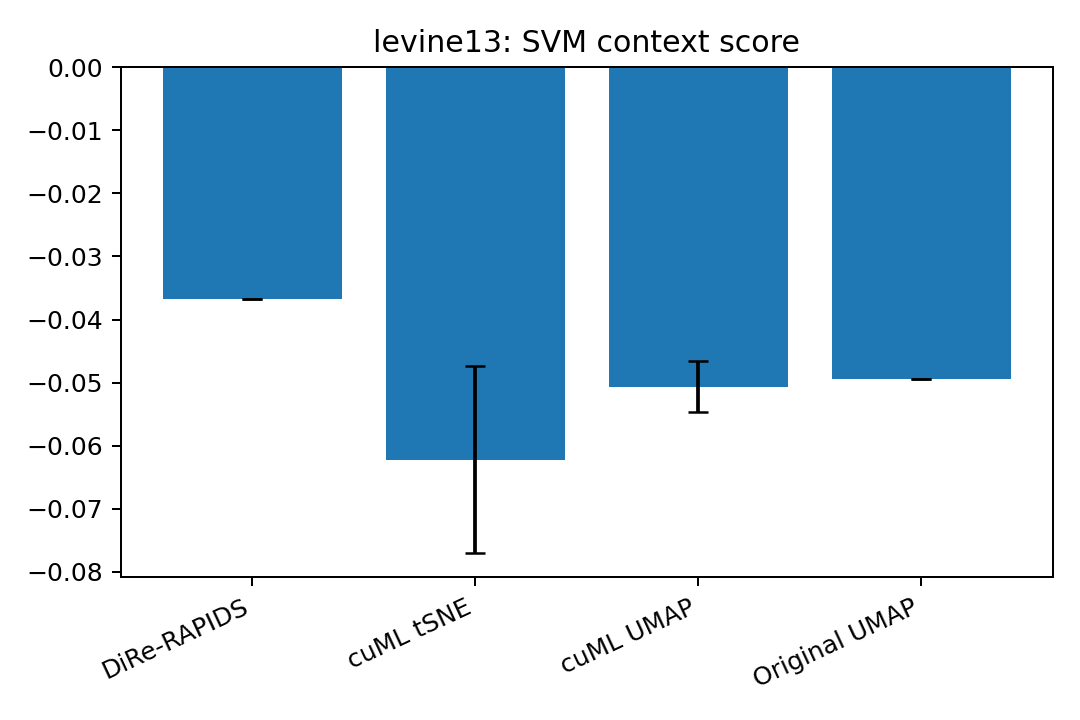
\includegraphics[width=\textwidth]{pics/levine13_comparison/levine13-context.png}
        \caption{SVM context score}
        \label{fig:levine13-context}
    \end{subfigure}
    \hfill
    \begin{subfigure}[b]{0.35\textwidth}
        \centering
        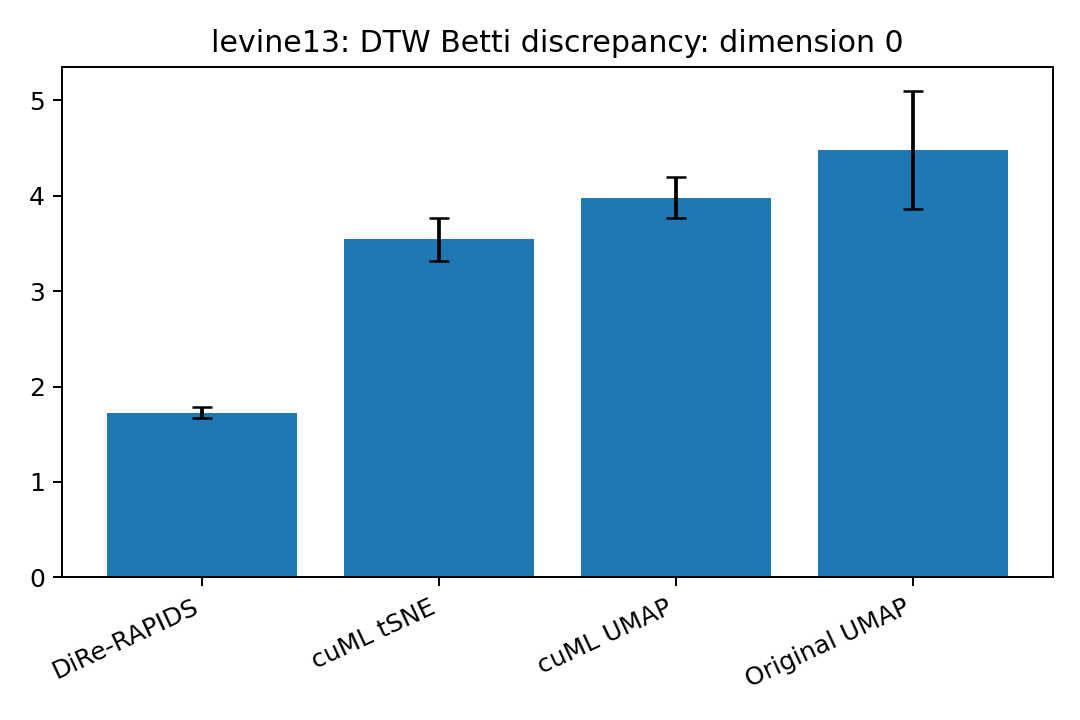
\includegraphics[width=\textwidth]{pics/levine13_comparison/levine13-persistence-dim-0.png}
        \caption{DTW Betti discrepancy: dimension $0$}
        \label{fig:levine13-persistence-0}
    \end{subfigure}
    \hfill
    \begin{subfigure}[b]{0.35\textwidth}
        \centering
        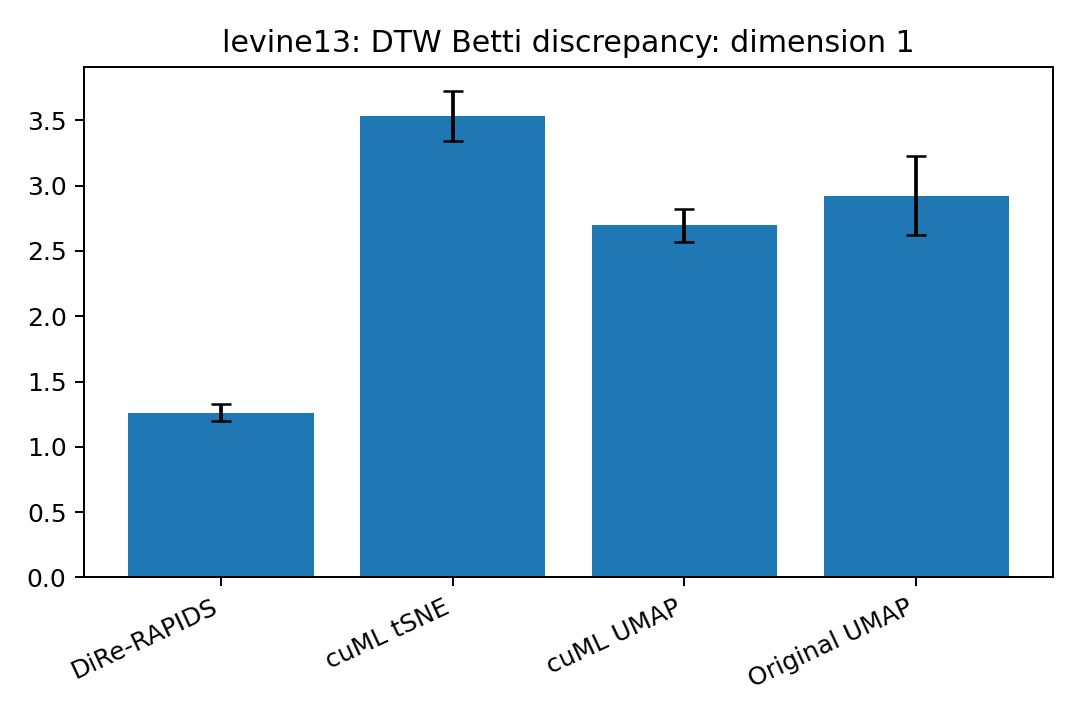
\includegraphics[width=\textwidth]{pics/levine13_comparison/levine13-persistence-dim-1.png}
        \caption{DTW Betti discrepancy: dimension $1$}
        \label{fig:levine13-persistence-1}
    \end{subfigure}
    \caption{"Levine 13" dataset metrics comparison. Error bars show sample standard deviations.}
    \label{fig:levine13-comparison}
\end{figure}

\newpage 

\section{Levine 32: Dataset Metrics}\label{appendix:levine32}


\begin{figure}[ht]
    \centering
    \begin{subfigure}[b]{0.35\textwidth}
        \centering
        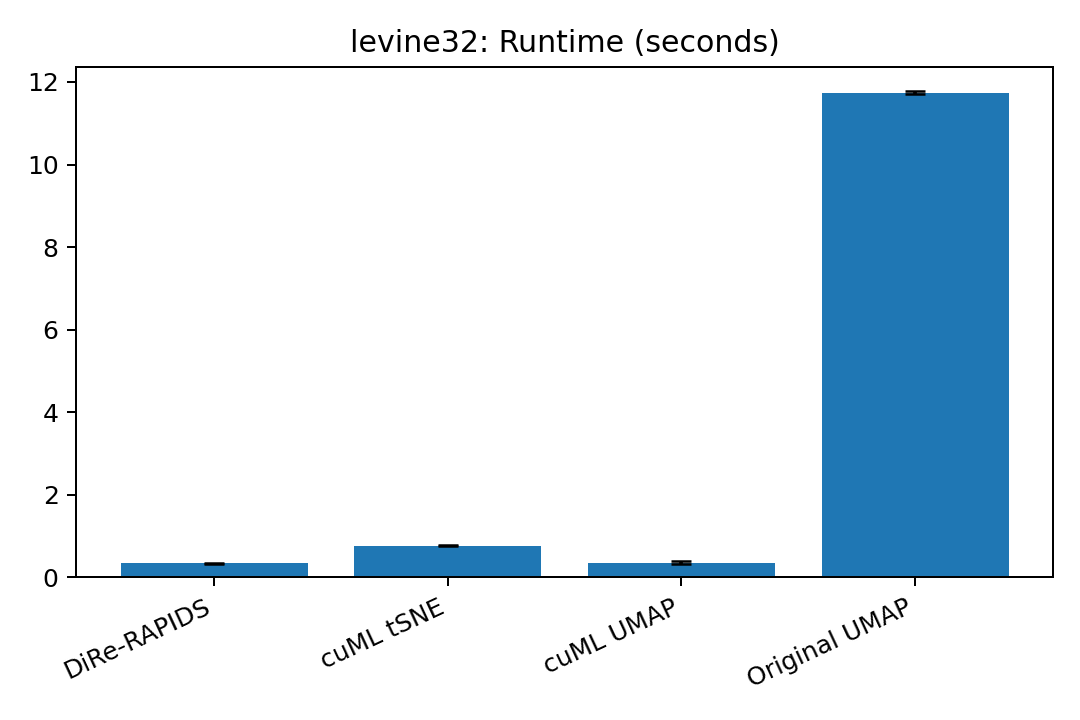
\includegraphics[width=\textwidth]{pics/levine32_comparison/levine32-time.png}
        \caption{Runtime (seconds)}
        \label{fig:levine32-time}
    \end{subfigure}
    \hfill
    \begin{subfigure}[b]{0.35\textwidth}
        \centering
        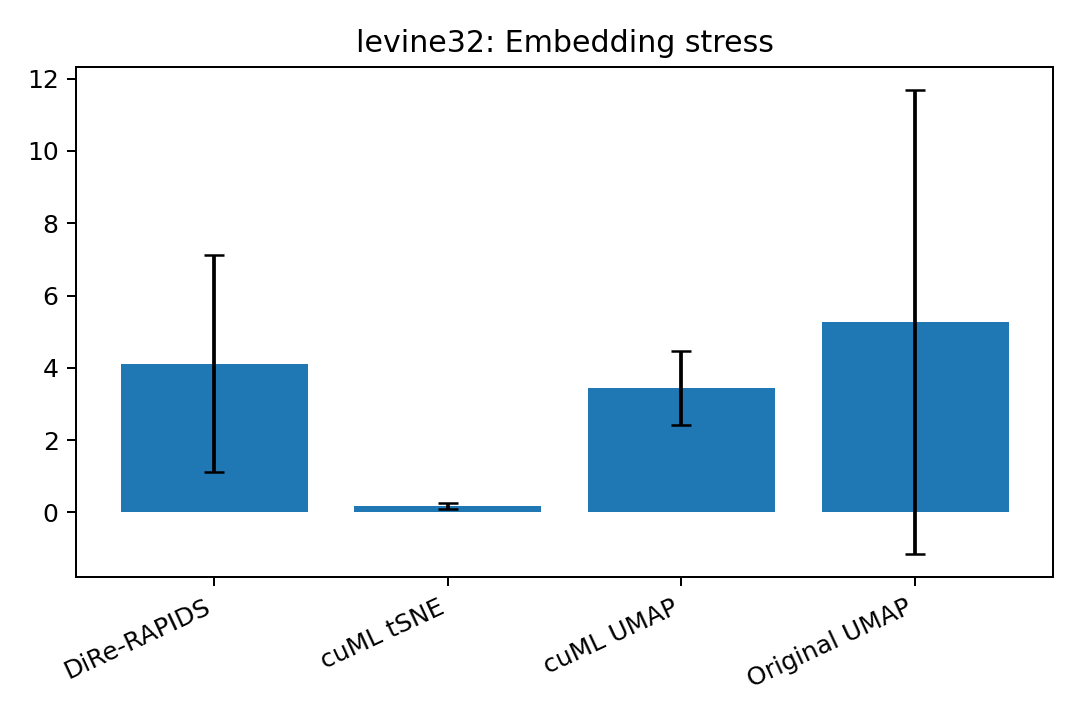
\includegraphics[width=\textwidth]{pics/levine32_comparison/levine32-stress.png}
        \caption{Embedding stress}
        \label{fig:levine32-stress}
    \end{subfigure}
    \vspace{1em}
    \begin{subfigure}[b]{0.35\textwidth}
        \centering
        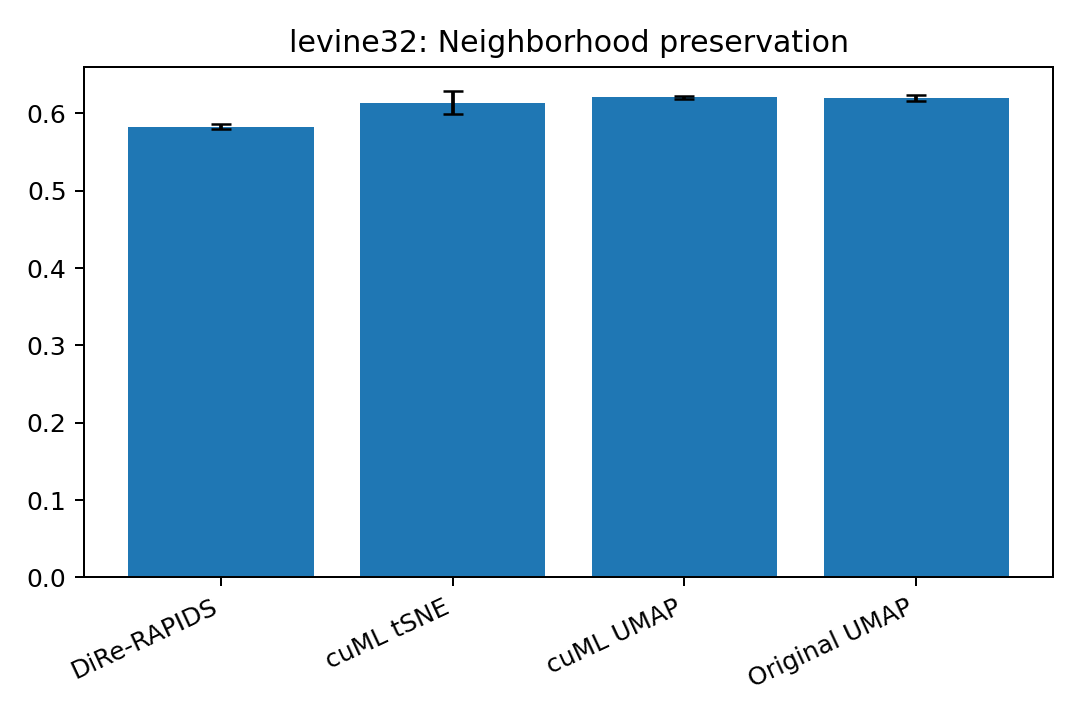
\includegraphics[width=\textwidth]{pics/levine32_comparison/levine32-neighborhood.png}
        \caption{Neighborhood preservation}
        \label{fig:levine32-neighborhood}
    \end{subfigure}
    \hfill
    \begin{subfigure}[b]{0.35\textwidth}
        \centering
        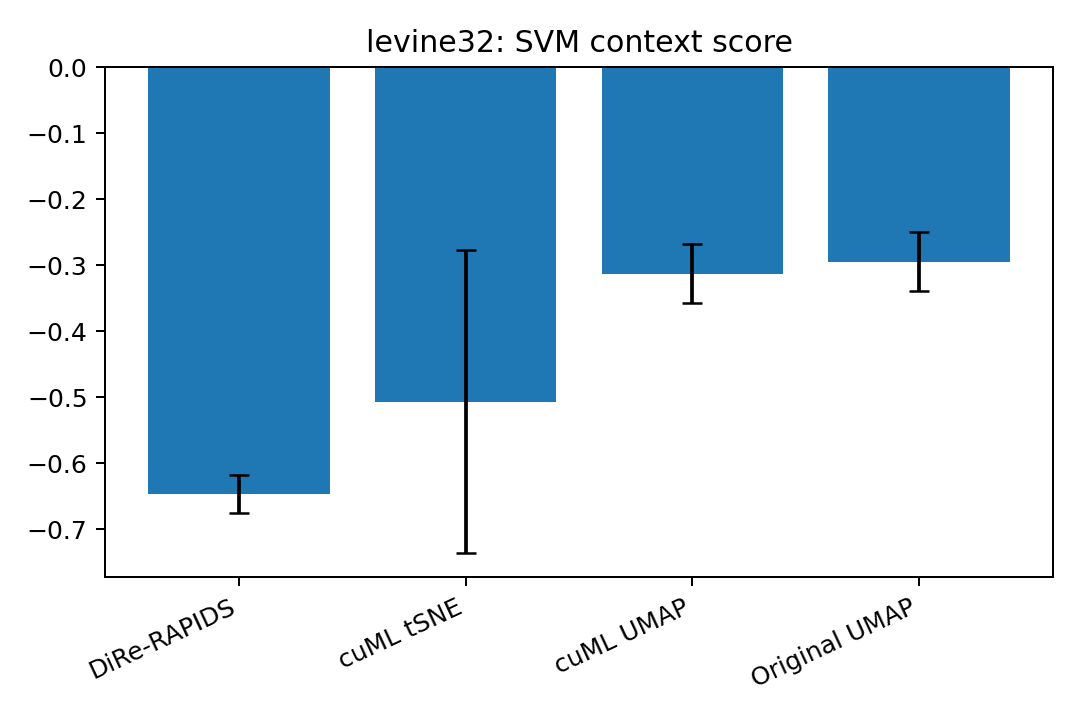
\includegraphics[width=\textwidth]{pics/levine32_comparison/levine32-context.png}
        \caption{SVM context score}
        \label{fig:levine32-context}
    \end{subfigure}
    \hfill
    \begin{subfigure}[b]{0.35\textwidth}
        \centering
        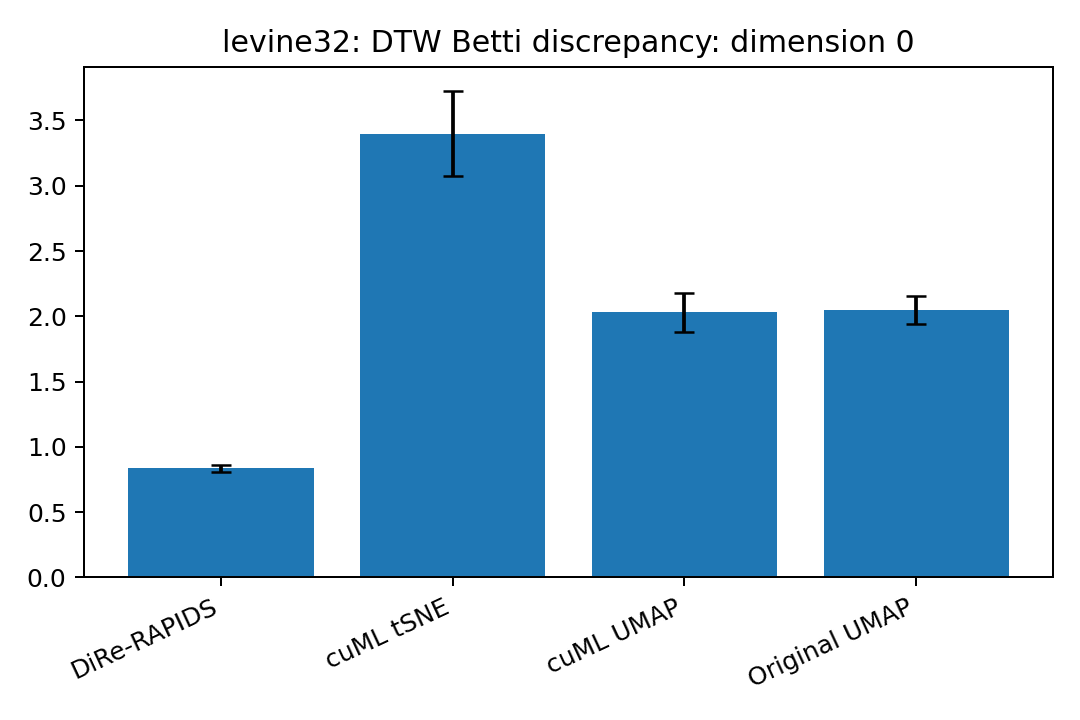
\includegraphics[width=\textwidth]{pics/levine32_comparison/levine32-persistence-dim-0.png}
        \caption{DTW Betti discrepancy: dimension $0$}
        \label{fig:levine32-persistence-0}
    \end{subfigure}
    \hfill
    \begin{subfigure}[b]{0.35\textwidth}
        \centering
        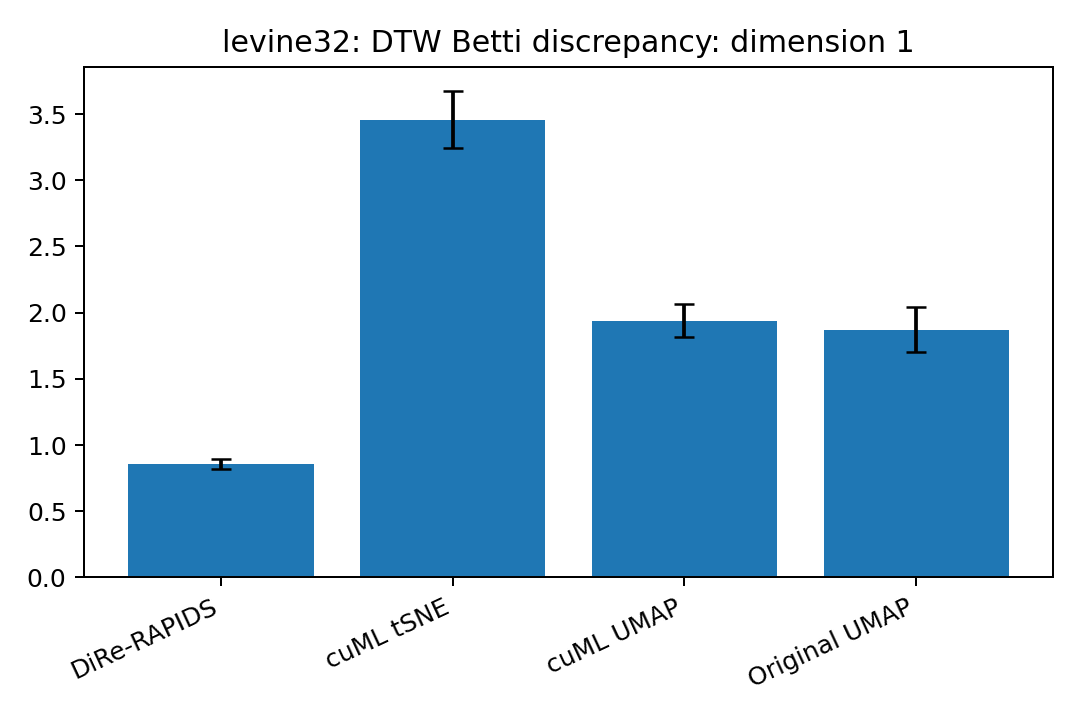
\includegraphics[width=\textwidth]{pics/levine32_comparison/levine32-persistence-dim-1.png}
        \caption{DTW Betti discrepancy: dimension $1$}
        \label{fig:levine32-persistence-1}
    \end{subfigure}
    \caption{"Levine 32" dataset metrics comparison. Error bars show sample standard deviations.}
    \label{fig:levine32-comparison}
\end{figure}

\end{document}
